\documentclass[12pt,a4paper]{article}
%%%%%%%%%%%%%%%%%%%%%%%%%%%%%%%%%%%%%%%%%%%%%%%%%%%%%
\usepackage[utf8]{inputenc}
% \usepackage[portuguese]{babel}
% \addto{\captionsportuguese}{%
%   \renewcommand{\refname}{\hfill \large References\hfill} % V V V
% }
% \addto{\captionsportuguese}{% 
%   \renewcommand{\contentsname}{\hfill Table of Contents \hfill}} %\centering não tava funcionando sabe deus por que, usei o \hfill pra enjambrar
        
\usepackage[T1]{fontenc}
\usepackage{fontspec}
\usepackage{pdflscape}
\usepackage{amsmath,esint}
\usepackage{amsfonts}

\usepackage{minted}
\newminted{python}{frame=lines,framerule=2pt}

\usepackage{amssymb}
\usepackage{makeidx}
\usepackage{graphicx}
\usepackage{array}
\usepackage{tabularray}
\usepackage{lettrine}
\usepackage{lmodern}
\usepackage[table]{xcolor} 
% \usepackage{dirtytalk}
% \usepackage{setspace}
\usepackage{float}
    % \linespread{1.5}
    \linespread{1.25} % about 1.5 spacing in Word
\setlength{\parindent}{0pt} % no paragraph indents
\setlength{\parskip}{1em} % paragraphs separated by 
% one line
% \usepackage{indentfirst}
%     \setlength{\parindent}{1cm}
%     \setlength{\parskip}{0pt}
\usepackage{pdfpages}
\usepackage[left=2cm,right=2cm,top=2cm,bottom=2cm]{geometry}
\usepackage{hyperref}
\usepackage{multirow}
% \usepackage{booktabs}
% \usepackage{caption}
% \usepackage{subfigure}
\usepackage{subcaption}
\usepackage{fancyhdr}
\usepackage{tabularray}
\usepackage{soul} % Pacote que permite grifar palavras no texto

\usepackage[ %faz a citação ser do tipo autor data, faz parecer et al na citação, mas na referencia mostra todos os autores e deixa o titulo em negrito na referencia
	alf,
	abnt-repeated-title-omit=yes,	
	abnt-emphasize=bf,
	abnt-etal-list=0
	]
	{abntex2cite}
\citebrackets()%faz a citação ser entre parenteses e não entre colchetes

%-----------------------------------------------------------
\hypersetup{
%links coloridos
   pdfborder={0 0 0},
   colorlinks = true,  
   linkcolor = black,          % Cor dos links internos
   citecolor = blue        % Cor dos links das referências bibliográficas
}
\setmainfont{Times New Roman}
\pagestyle{fancy}
% Clear the header and footer
\fancyhead{}
\fancyfoot{}
\fancyhead[R]{\thepage}
\renewcommand{\headrulewidth}{0pt}%
\setlength{\headheight}{14.49998pt}
%-----------------------------------------------------------

%------Redefinido Tamanho de Fontes-------------------------

\renewcommand{\large}{\fontsize{14}{15}\selectfont}  % large vira 14pt
\usepackage{titlesec}
    \titleformat{\section}
      {\normalfont\fontsize{14}{15}\bfseries}{\thesection}{1em}{}
\newcommand\GroupName{Richa Patel s4581307} %%%%% Put 
%-----------------------------------------------------------
\setcounter{page}{1}
\pagestyle{fancy}
\fancyhf{}
\rhead{\thepage}
\lhead{\GroupName}

\begin{document}

%___________________________CAPA___________________________%
    \begin{titlepage}

        \begin{center}
                \textbf{UNIVERISTY OF QUEENSLAND }
        \end{center}
   
    \vspace*{2cm}
   \begin{center} % Adjust spacings to ensure the title page is generally filled with text
        \Huge{\textbf{COSC3000\\}}
        \LARGE{\color{teal}{VISUALISATION PROJECT}}\\
        \vspace{0.4cm}
        \textbf{Commercial Whaling 1985-2018}\\
        \vspace{0.1 cm}
        \Large{$28^{th}$ April, 2023}
    \end{center}

    
    \vspace*{5cm}

    \begin{center}
    \large
         \textbf{By Richa Patel}
    \end{center}
      
    % \vfill  
    
    % \begin{center}
    %     \textbf{Rio do Sul}

    %     \textbf{ano}
        
    % \end{center}
    
    

    \end{titlepage}



% %______________________Folha de Rosto__________________________%

% \thispagestyle{empty} %sem numeração de página

%     \begin{center}
%         \textbf{NOME}
%     \end{center}

%     \vspace{3 cm}

%     \begin{center}
%         \large
%         \textbf{TÍTULO DO RELATÓRIO DE ESTÁGIO}
%     \end{center}

%     \vspace{3 cm}
    
%     \hfill\begin{minipage}{\dimexpr\textwidth-8,5 cm}
%         \linespread{1,0}\selectfont
%         \large 
%             Relatório de Estágio Supervisionado I do Curso de Licenciatura em Física do Instituto Federal Catarinense Campus Rio do Sul realizado na Escola XXXXXXXXXXX,  como requisito parcial para conclusão da disciplina de Estágio Supervisionado I.\\

%             Professor Orientador: XXX

%     \xdef\tpd{\the\prevdepth}
%     \end{minipage}

%     \vfill

%     \begin{center}
%         \textbf{Rio do Sul\\
%         Ano}
%     \end{center}





% \newpage

% %______________________Folha em Branco__________________________%
% \thispagestyle{empty} 

% \

\newpage

%______________________________Sumário_________________________%
\thispagestyle{empty} 
\tableofcontents
\newpage
%_____________________________Introdução__________________________%
\section{Introduction}
\subsection{Background}
Human impacts on marine ecosystems have been a long-standing and pressing issue. These are as a result of direct human activities such as overfishing, oil drilling, transportation, and more. Along with indirect impacts resulting in rising sea temperatures and levels. 

One of the more pressing matters appearing recently in the public discourse is commercial whaling. Commercial whaling began quite early in the 1600s, as a source of whale blubber was utilised in a wide range of products. However, by the late 1940s, the whale population saw an immense decline. Resulting in the formation of the International Whaling Commission. 

\textbf{EDIT HERE}
\subsection{Data Description}
The data set utilised is from the International Whaling Commissions public data archive on whaling from 1985 to 2018 which can be accessed \textbf{here}. As a result, providing a comprehensive overview about the countries involved, the areas whaling occured and the species. 

The table below provides further details on the description of each of the data labels and features. (Refer to Table \ref{tab:table1}) 

\begin{table}[H]
\rowcolors[]{1}{white}{teal!10}
\centering
\begin{tabular}{| m{5cm} |m{10cm}|}
\hline
 \textbf{Data Label} & \textbf{Description}\\ 
 \hline
    Year
  & 
  Years from 1985 to 2018
\\ 
 \hline
 Nation
  &   Nations/ countries involved in Commercial Whaling \\ 
 \hline
 Type
 & Types are broken into \\ 
 \hline
  Overflow Flag = $1$, 
  Overflow Flag = $0$, 
 & Set\\ 
 \hline
  Zero Flag = $1$, 
  Zero Flag = $0$, 
 & Set Input A and B, to all 0's (test trival output), then test same inputs with $Cin = 1$, $Cin = 0$ , $Sat = 1$ and $Sat = 0$.\\
   \hline
\end{tabular}
 \caption{\label{tab:table1} Description of Data Attributes and Feature Labels}
\end{table}

The nature of the data set on initial observation provides a number of opportunities on potential visualisation to better gauge how whales are being impacted by commercial whaling and the patterns and behaviours of each Nation's whaling endeavours. This consists of a time series analysis, along with geographical and spatial visualisations. Furthermore, to directly emphasise the human impact element of commercial whaling an assisting data set from the Global Cetecean Summary Report, published by the Australian Government Department of Environment,  Water, Heritage and Arts - June 2009 has been included. This data set highlights the IUCN's Threatened Species criteria value for various Cetecean species.  The table below provides further details on the description of each of the data labels and features. (Refer to Table \ref{tab:table1})

\begin{table}[H]
\rowcolors[]{1}{white}{teal!10}
\centering
\begin{tabular}{| m{5cm} |m{10cm}|}
\hline
 \textbf{Data Label} & \textbf{Description}\\ 
 \hline
    Year
  & 
  Years from 1985 to 2018
\\ 
 \hline
 Nation
  &   Nations/ countries involved in Commercial Whaling \\ 
 \hline
 Type
 & Types are broken into \\ 
 \hline
  Overflow Flag = $1$, 
  Overflow Flag = $0$, 
 & Set\\ 
 \hline
  Zero Flag = $1$, 
  Zero Flag = $0$, 
 & Set Input A and B, to all 0's (test trival output), then test same inputs with $Cin = 1$, $Cin = 0$ , $Sat = 1$ and $Sat = 0$.\\
   \hline
\end{tabular}
 \caption{\label{tab:table2} Description of Data Attributes and Feature Labels}
\end{table}


\newpage


%_______________A ESCOLA CAMPO DE ATUAÇÃO DOCENTE____________%
\section{Project Outline and Aims}

    \subsection{Outline}
    The data visualisation shall primarily be conducted utilising Python libraries. Namely, Plotly, which is an interactive and robust visualisation tool. Along with Plotly Dash, which has been incorporated considering the data's time series nature where the ability to  visualise the data at particular points in time would require a level of interactivity. Along with assisting Python libraries such as Pandas, Matplotlib and Statsmodel API library to manipulate the data set for selective visualisations. 

    \subsection{Aims}
    
    The project aims to inform individuals on the nature of whaling and how it was conducted across time. Furthermore, it intends to  raise awareness on how certain species have been affected by whaling endeavors of particular Nations. This shall be achieved through analysing the data's complex behavior across space and correlating this with the species endangerment data set. Additionally, the project intends to investigate correlations between various feature sets across the data set. 
    Along with applying data analysis techniques to observe various species' distribution across time.  Moreover, the visualisation aims to provide a comprehensive overview by providing visualisations across each point in time and a cumulative overview. This allows the progression of whaling to be observed, along with each Nation's overall impact. In order to achieve this animation and interactive features shall be incorporated. Lastly, the visualisations intend to provide flexibility in order to cater for a larger audience, providing ease of on-screen viewing and viewing for individuals with visual impairments. 
    
    % The visualisation aims to reduce the complexity of the data set by providing an interactive time series animation and slider to allow people to view the evolution of whaling from 1985 to 2018 for most visualisations. Along with a cumulative overview of the data across time from 1985 to 2018. Lastly, the visualisation intends to provide flexibility in order to cater 

\section{Data Analysis}
Upon exploratory analysis, it was observed that the data can be manipulated into a univariate, bivariate, or multivariate form. However, the univariate data would require several assisting visualisations in order to holistically represent data. As a result, it was devised to focus more on how to visualise the dependencies between the feature sets of the data, representing this with multivariate visualisations, and including supporting univariate or bivariate visualisations. 

 \subsubsection{Visualisations}
    The scope of visualisations that shall be provided considering the nature of the data set consists of: 
\begin{enumerate}
  \item Geospatial Visualisation \\
  \item Feature Correlation Visualisations\\
  \item Categorical Visualisations\\
  \item Species Distribution Analysis
\end{enumerate}
  
\newpage


\section{Data Preparation}
Due to the complex nature of the data set, some preprocessing was conducted in order to assist in simplifying the data. Firstly, the years 1985 and 1986 contain data labels with the name USSR as a Nation category which has been equated to Russia for completeness purposes. Along with ease in determining the Geographical polygon for the geospatial visualisation. Moreover, the 'Type' category had some inconsistencies with labels of the same value being capitalised resulting in duplicate values. This was rectified by setting all labels to be of sentence case type. 

The following code highlights how these changes were implemented. 

\begin{minted}[frame=single,framesep=4pt,fontsize=\small]{python}
original_df = pd.read_csv("Project\\WhalingData.csv").dropna()
original_df['Nation'].replace({"USSR": "Russia"}, inplace=True)
original_df['Type'] = original_df['Type'].str.title()
\end{minted}

Furthermore, additional data retrieval had to be conducted to obtain longitude and latitude coordinates for the 'Areas' category. This data was then comprised into a separate data set. Moreover, the IUCN's Endangered Species Red List data set where certain whale species were listed as data deficient in the report, therefore were not included in the data set. To compensate for this an additional category devised as 'UN' has been included for the Minke and Bryde's species.  The data sets have been provided in Appendix A and B respectively.  

Retrieval of longitude and latitude coordinates was achieved using Google Earth, obtaining the coordinates and creating a separate data set that obtained the Area with its corresponding latitude and longitude coordinates. Analogously a data deficient category ('UN') was included in the Red List data set for completeness purposes.


\section{Multivariate Visualisations}
\subsection{Geographic Visualisation}

The first multivariate visualisation consisted of encompassing the geographical features of the data set, which was best represented using a Choropleth plot. This visualisation also provides a level of interactivity, allowing the user to observe the data at a particular point in time, by selecting a slider value or cumulative totals for each region combining all points in time, by selecting the 'ALL' checkbox. Along with an animation feature, by selecting the 'ANIMATE' check box. This provides the ability to observe the changes across time and visualise the progression of whaling more efectively. 

The following code highlights the data retrieval and manipulation process. The first data frame was utilised to group the data by year and nation, where each year is filtered by the interactive slider. The second data frame encompasses the aggregate data across all time. 

\begin{minted}[frame=single,framesep=4pt,fontsize=\small]{python}
#Choropleth Plot Data
# Group the dataframe by Year and Nation 
df = original_df.groupby(['Year','Nation'])['Fin', 'Sperm', 
'Humpback', 'Sei', 'Bryde\'s', 'Minke', 'Gray', 'Bowhead', 
'Total'].sum().reset_index()
#Choropleth Plot Data - ALL
df_world_comb = original_df.groupby(['Nation'])['Total'].sum().reset_index()
\end{minted}

The Choropleth plot utilises 3 main features, the Nation's GeoJson polygon, the Nation's ISO 3166-1 alpha-3 codes, and the 'Total' attribute column's data to evaluate on. Each Nation's GeoJson polygon was obtained from the following data archive : \url{https://raw.githubusercontent.com/python-visualization/folium/master/examples/data/world-countries.json}, where polygons provide map outlines of each Nation. The ISO 3166-1 alpha-3 codes were evaluated using Python's latest PyCountry library. The GeoJson polygons are then mapped, based on which  ISO 3166-1 alpha-3 code is provided.  The code for obtaining the ISO 3166-1 alpha-3 has been provided in Appendix C, where an additional column was added to the data frame. The final visualisation has been provided in Figure \ref{fig:world_fig1}. 

\begin{minted}
#Obtain alpha code and create column in data frames[frame=single,framesep=4pt,fontsize=\small]{python}
df['CODE']=alpha3code(df['Nation'])
df_world_comb['CODE'] = alpha3code(df_world_comb['Nation'])
\end{minted}

\begin{figure}[H]
    \centering
    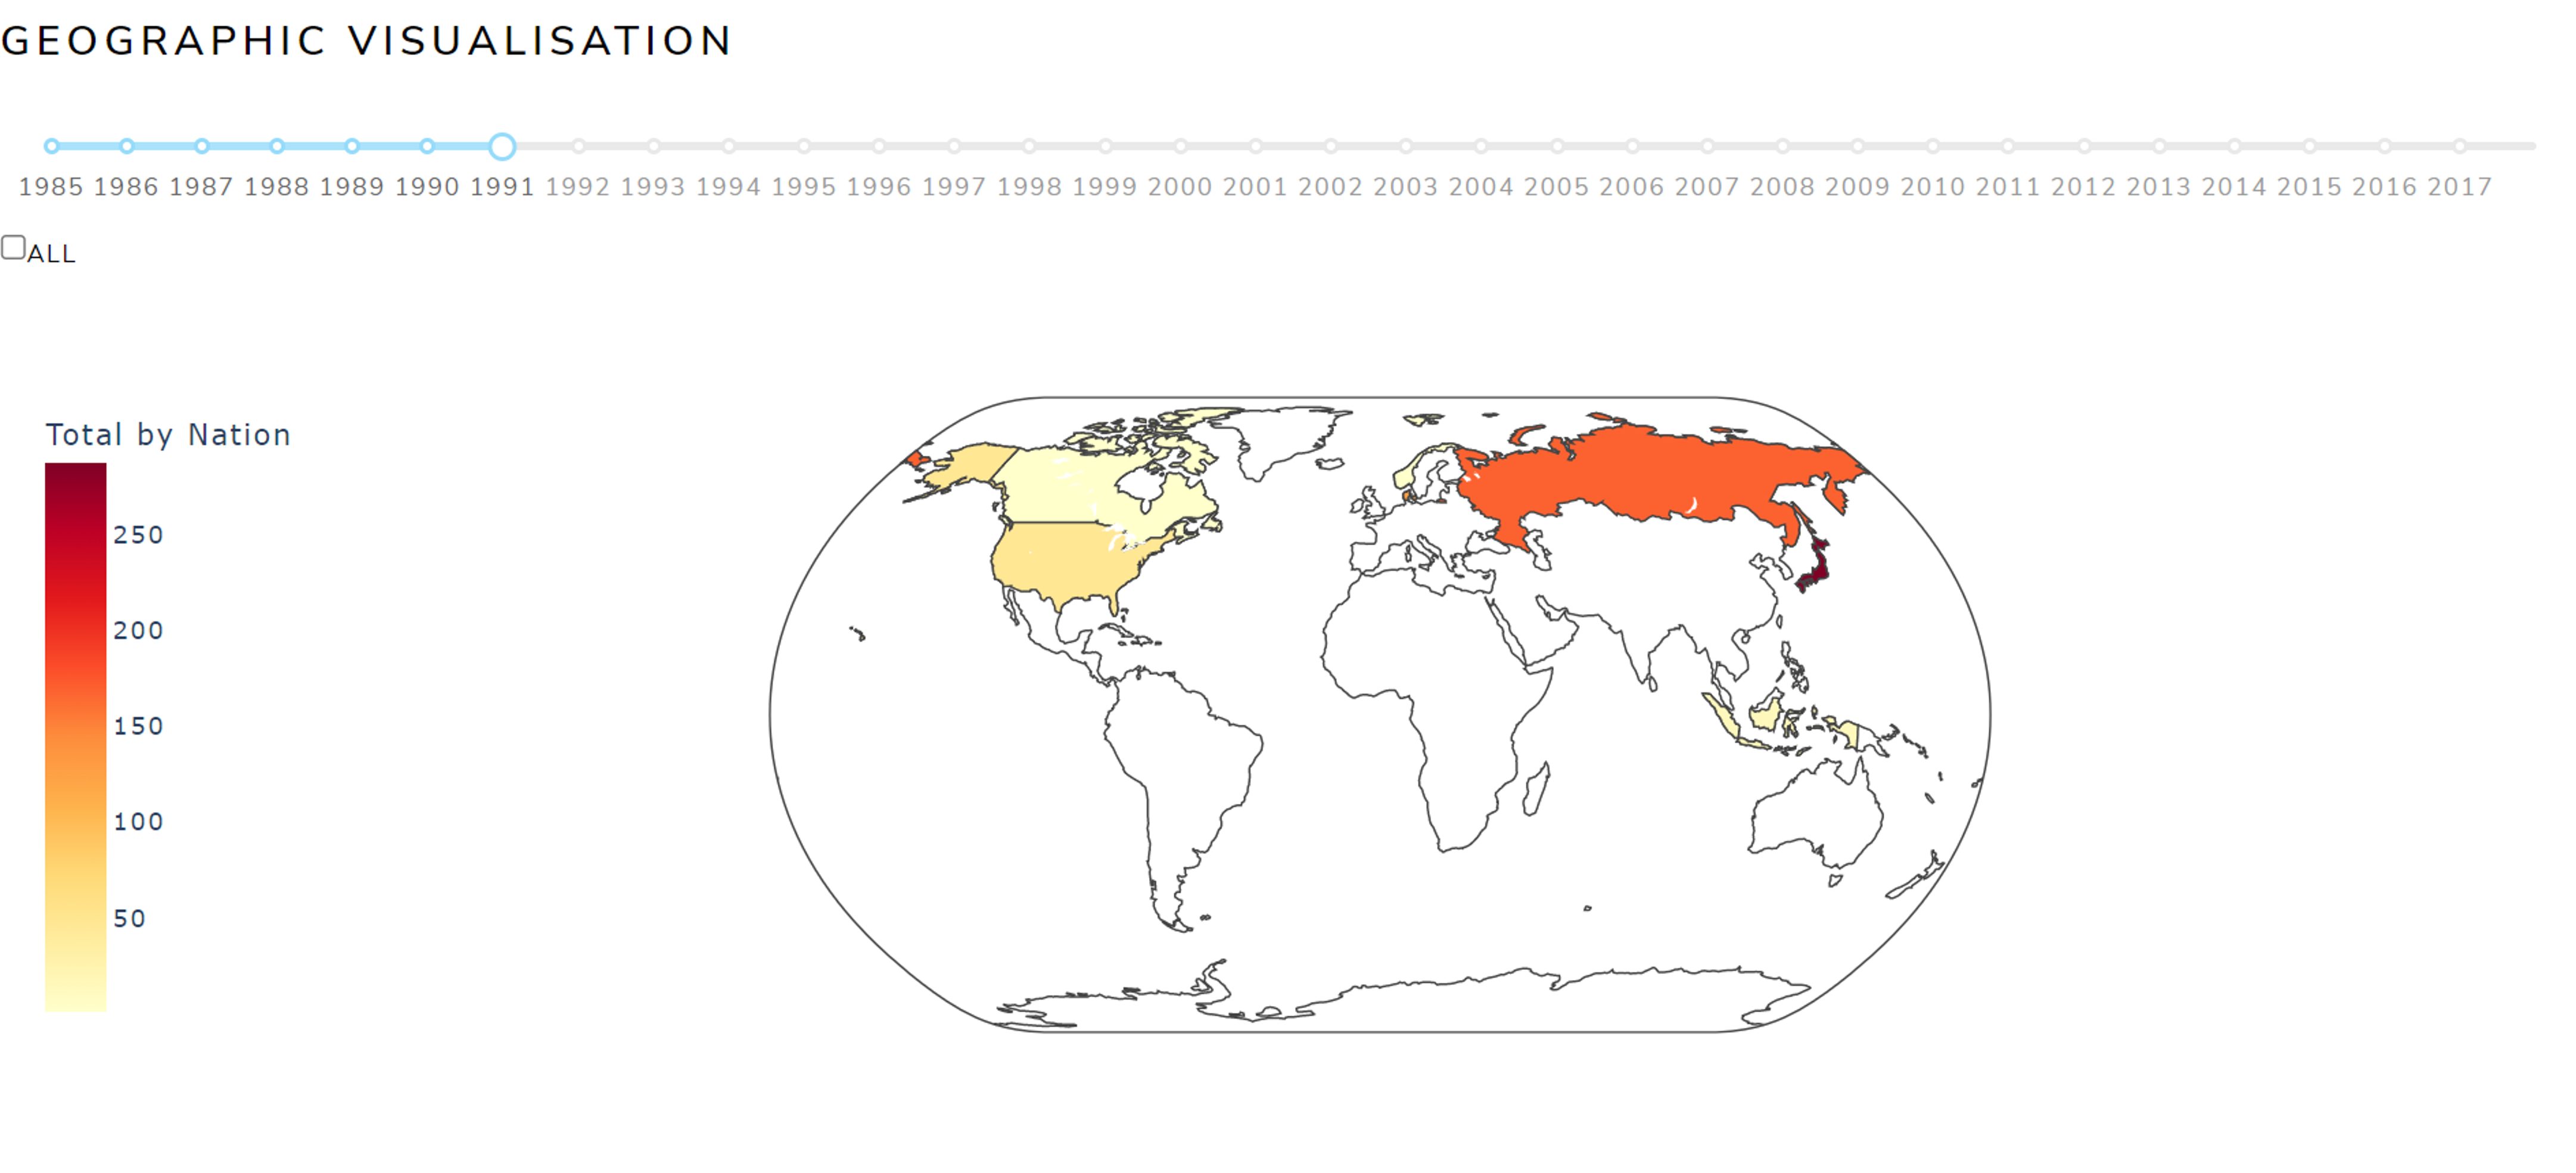
\includegraphics[width = 15cm]{Choropleth.png}
    \caption{Choropleth plot of whaling by Nation}
    \label{fig:world_fig1}
\end{figure}

The addition of the colour scale, provides insight on each Nation's total number of whales. However, this visualisation utilises univariate data, in order to encompass multivariate data the 'Area' category was included using the Geographical Scatter plot, where the two figures are combined into a single visualisation. 

\subsubsection{Choropleth Plot and Geographical Scatter Plot}
The Geographical Scatter plot utilises the gathered longitude and latitude coordinates, highlighting whaling that occurred for each area in a given year, and also the total across all years when the 'ALL' checkbox is selected. The longitude and latitude data set is provided in Appendix A was combined with the main whaling data set by including additional longitude and latitude coordinates.

The following code highlights the manipulation and retrieval of the data for this visualisation. 

\begin{minted}[frame=single,framesep=4pt,fontsize=\small]{python}
#Scatter Geo Data Grouping
df_1 = original_df.groupby(['Year','Nation','Area'])['Fin', 
'Sperm', 'Humpback', 'Sei', 'Bryde\'s', 'Minke', 'Gray', 
'Bowhead', 'Total'].sum().reset_index()

#Scatter Geo Data - ALL
df_1_combined = original_df.groupby(['Nation','Area'])
['Total'].sum().reset_index()
\end{minted}


The scatter plot points are coloured by which nation was responsible for whaling in this area. Whilst this could have been achieved by drawing plot lines from the Nation to each scatter point, this made the data visually more convoluted to read, due to a clustering of points. Therefore a colour legend was utilised, along with hover data labels, where more information is provided on hovering over the scatter points.  Additional interactive features were also included which includes the ability to rotate the map, zoom in and toggle legend items. (Refer to Figure \ref{fig:scattergeo})

\begin{figure}[H]
    \centering
    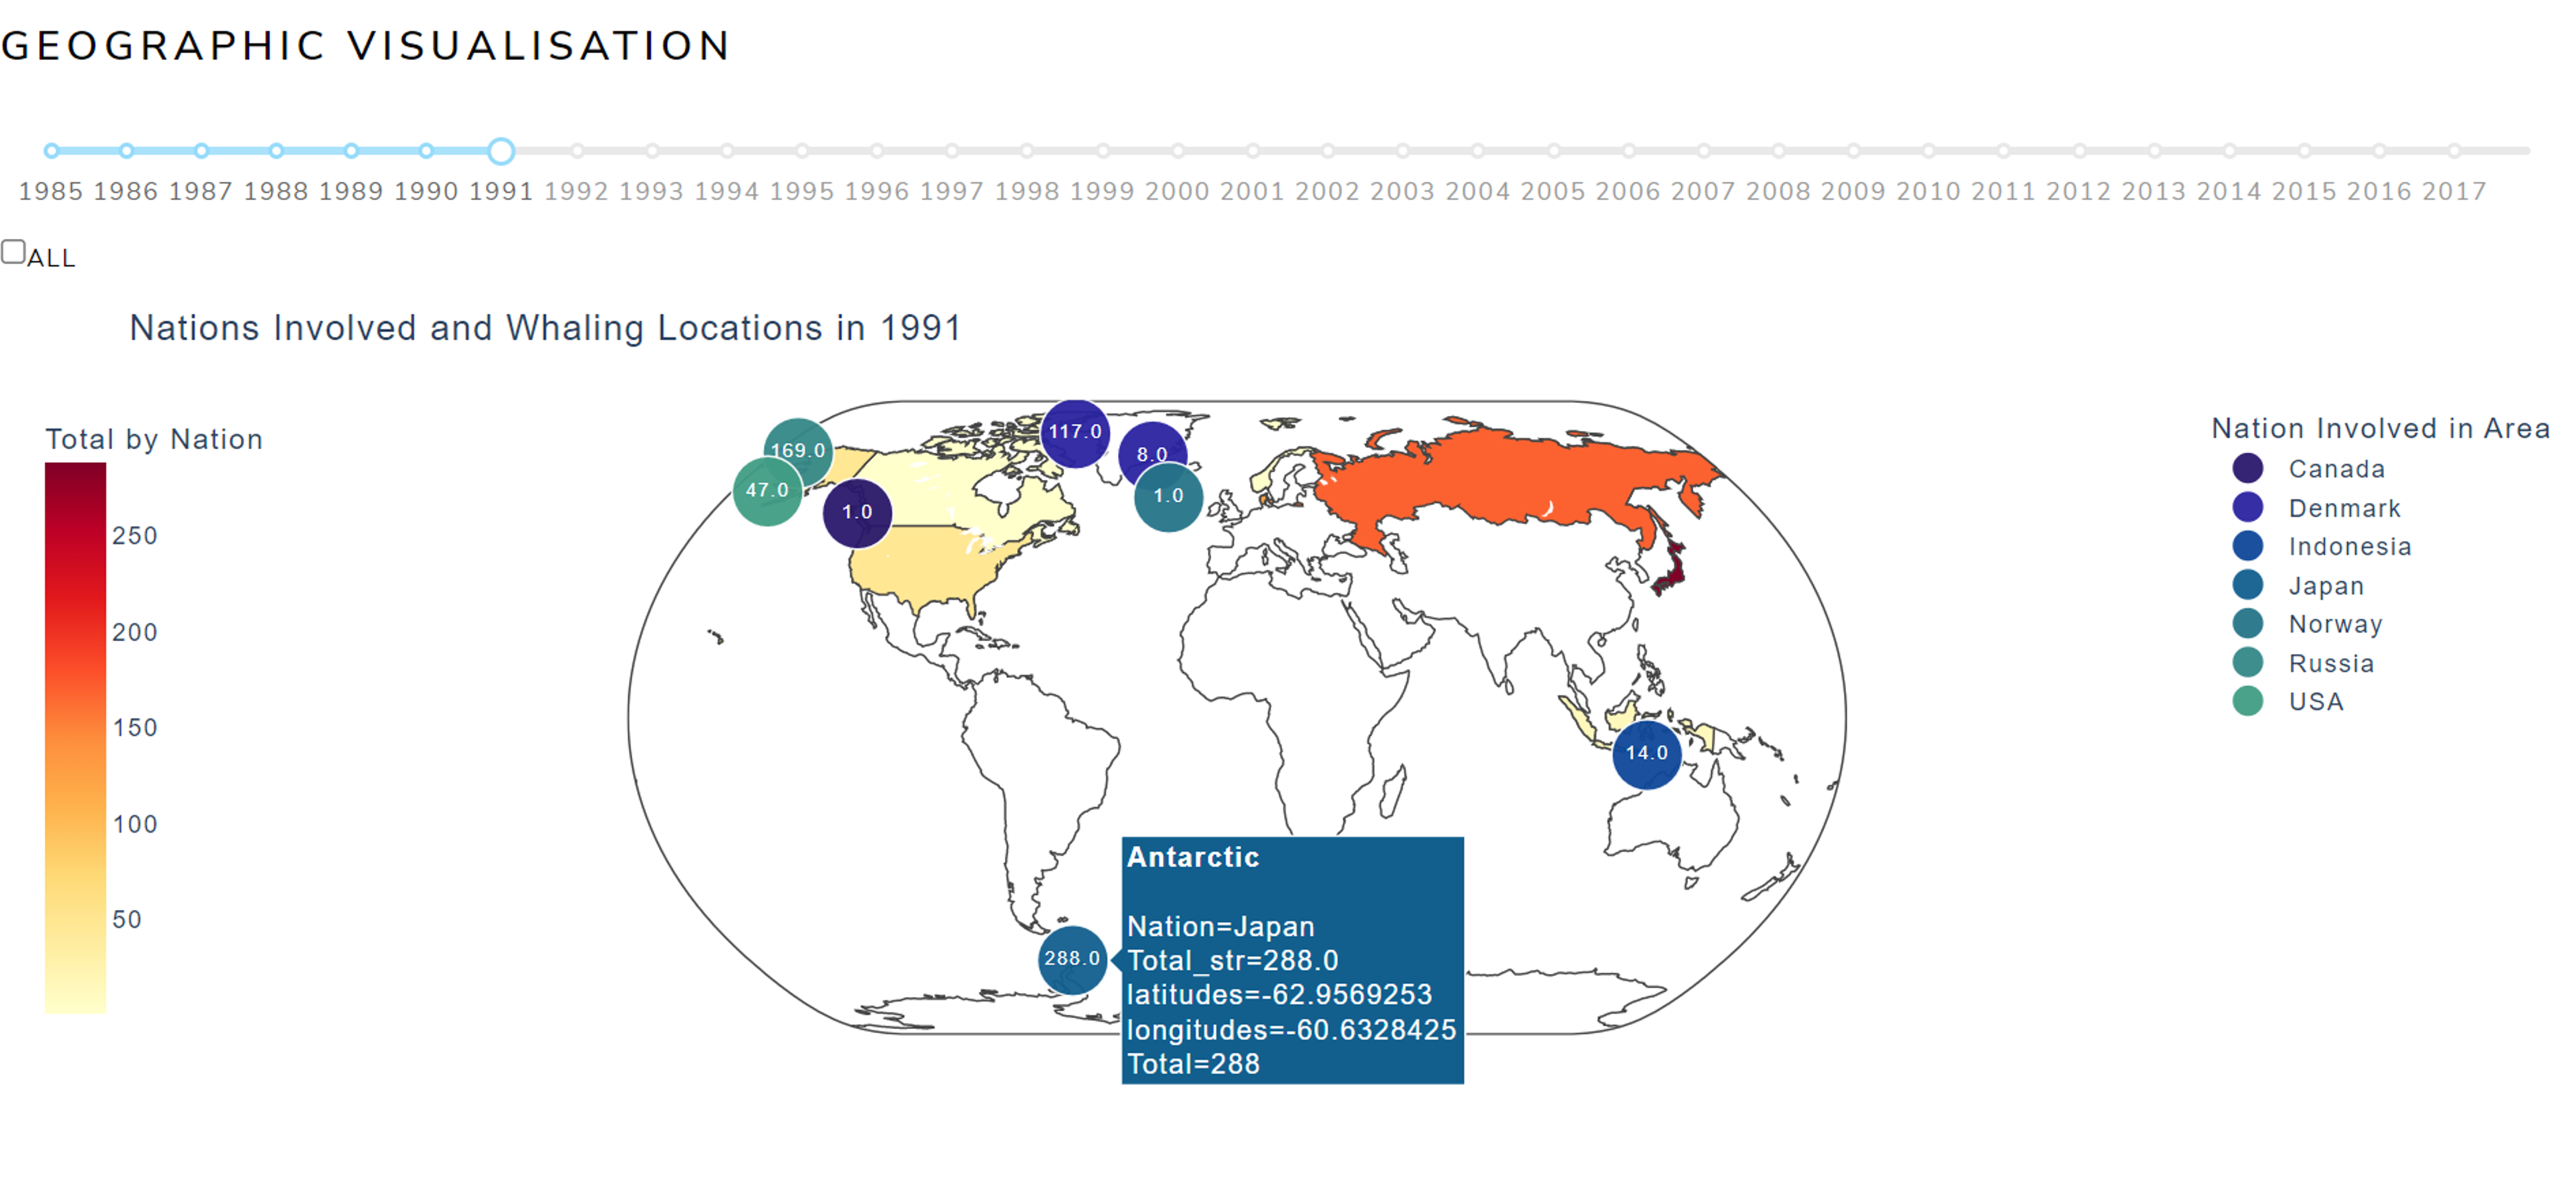
\includegraphics[width = 15cm]{FullChoro.png}
    \caption{Choropleth and Geographical scatter plot of global commercial whaling}
    \label{fig:scattergeo}
\end{figure}

\begin{figure}[H]
    \centering
    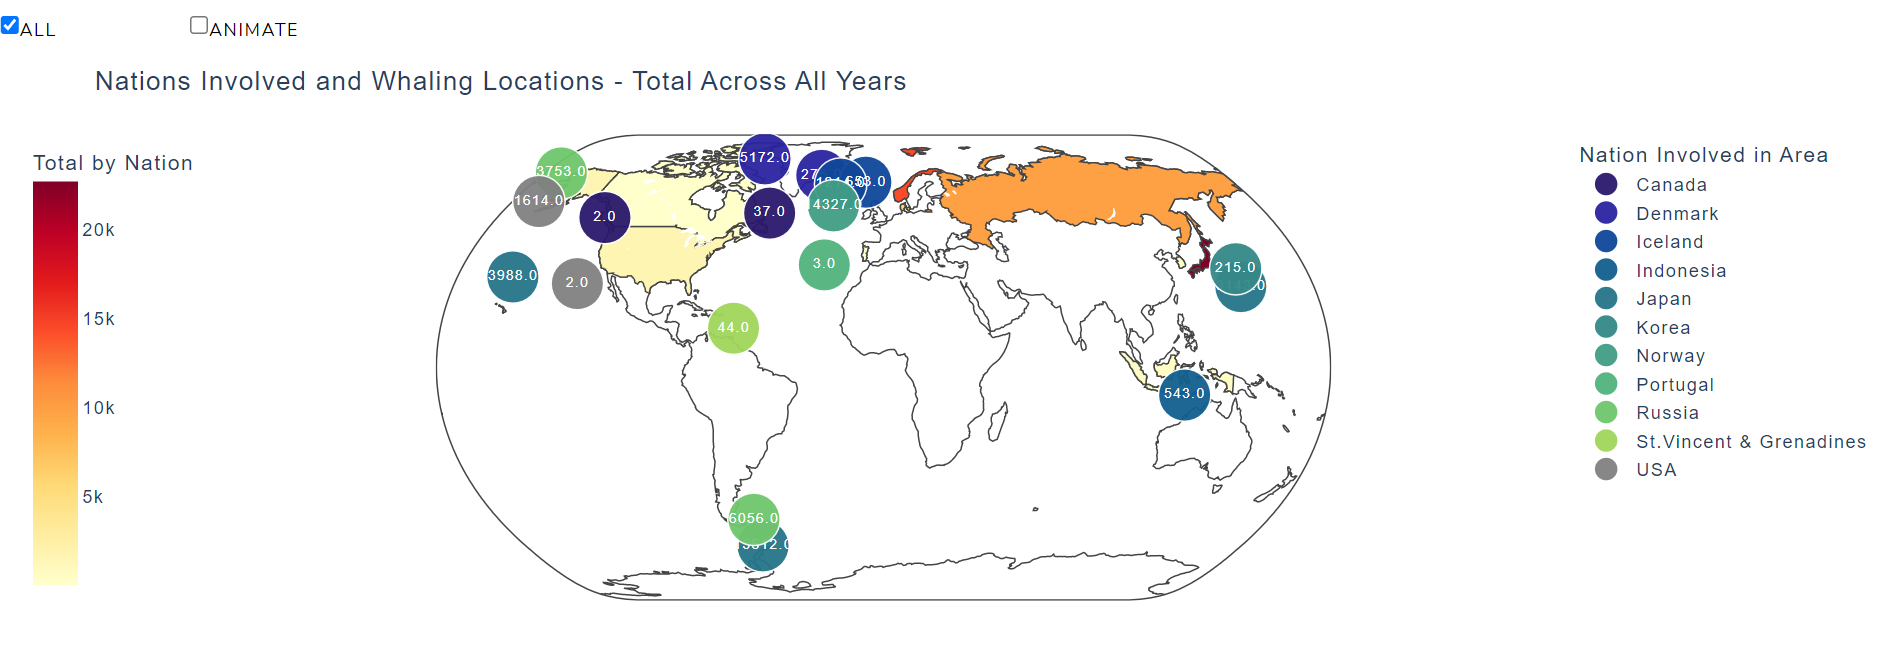
\includegraphics[width = 15cm]{fullChoroAll.png}
    \caption{Geographical and Correlation Map Visualisation Aggregate Data}
    \label{fig:fullChoroAll}
\end{figure}

\subsubsection{Evaluation}
The visualisation is successful in demonstrating the vast reach of commercial whaling across the globe, whilst emphasising regions  with larger clusters or volumes of whaling. The animation feature allows for the progression of whaling to be evaluated, where it's evidenced that the years 1990 to 2000 obtained the highest amount of activity across the globe. 

Moreover, the colour legend provides more details on how far particular nations would travel, with most Nations whaling within regional waters. However as indicated by Figure \ref{fig:fullChoroAll} Japan and Russia conducted their whaling missions mostly around Antarctica, with a cumulative 15,612 whales and 6052 whales respectively. This places Japan as the Nation contributing to the largest loss of whales as indicated by the colour scale, suggesting a total of above 20,000. 

 This further highlights why whaling sanctions had to be in place as nations would infiltrate non-regional waters, depleting whale numbers across the globe.  


\subsection{Feature Correlation Visualisations}
To further complement the geographic visualisation and explore other feature sets such as the type of whale and the species of whale, supporting feature correlation visualisations were created. 

\subsubsection{Species Type and Nation Correlation}

The species 'Type' category consists of the oceanic area the whale was located in and the type of whale. This may be either coastal whales, whales that prefer open water, migratory, infants or an unknown type. Further details are provided in table \ref{tab:table1}. 

Therefore correlating the type of whale with the nation, results in a three-dimensional data set, where a three-dimensional bar graph could be used to illustrate this categorical data, however, wouldn't complement the geographical visualisation being another complex visualisation. Moreover, it is much more difficult to gauge the height or actual value on a three-dimensional bar graph. As a result, a correlation map was utilised, where the colour scale correlates with the colour scale on the geographical plot. 

The species correlation map, further updates by year with the input slider bar, and also displays the cumulative totals when the 'ALL' checkbox is selected. The following code segment highlights column attributes used. The final visualisation is provided in Figure \ref{fig:heatmap1} and \ref{fig:heatmap2}

\begin{minted}[frame=single,framesep=4pt,fontsize=\small]{python}
#Correlation Map Data by Year
df_heatmap = original_df.groupby(['Year','Nation', 'Type']) 
['Total'].sum().reset_index()
#Correlation Map - ALL data
df_heatmap_total = original_df.groupby(['Nation', 'Type'])
['Total'].sum().reset_index()
\end{minted}

\begin{figure}[H]
    \centering
    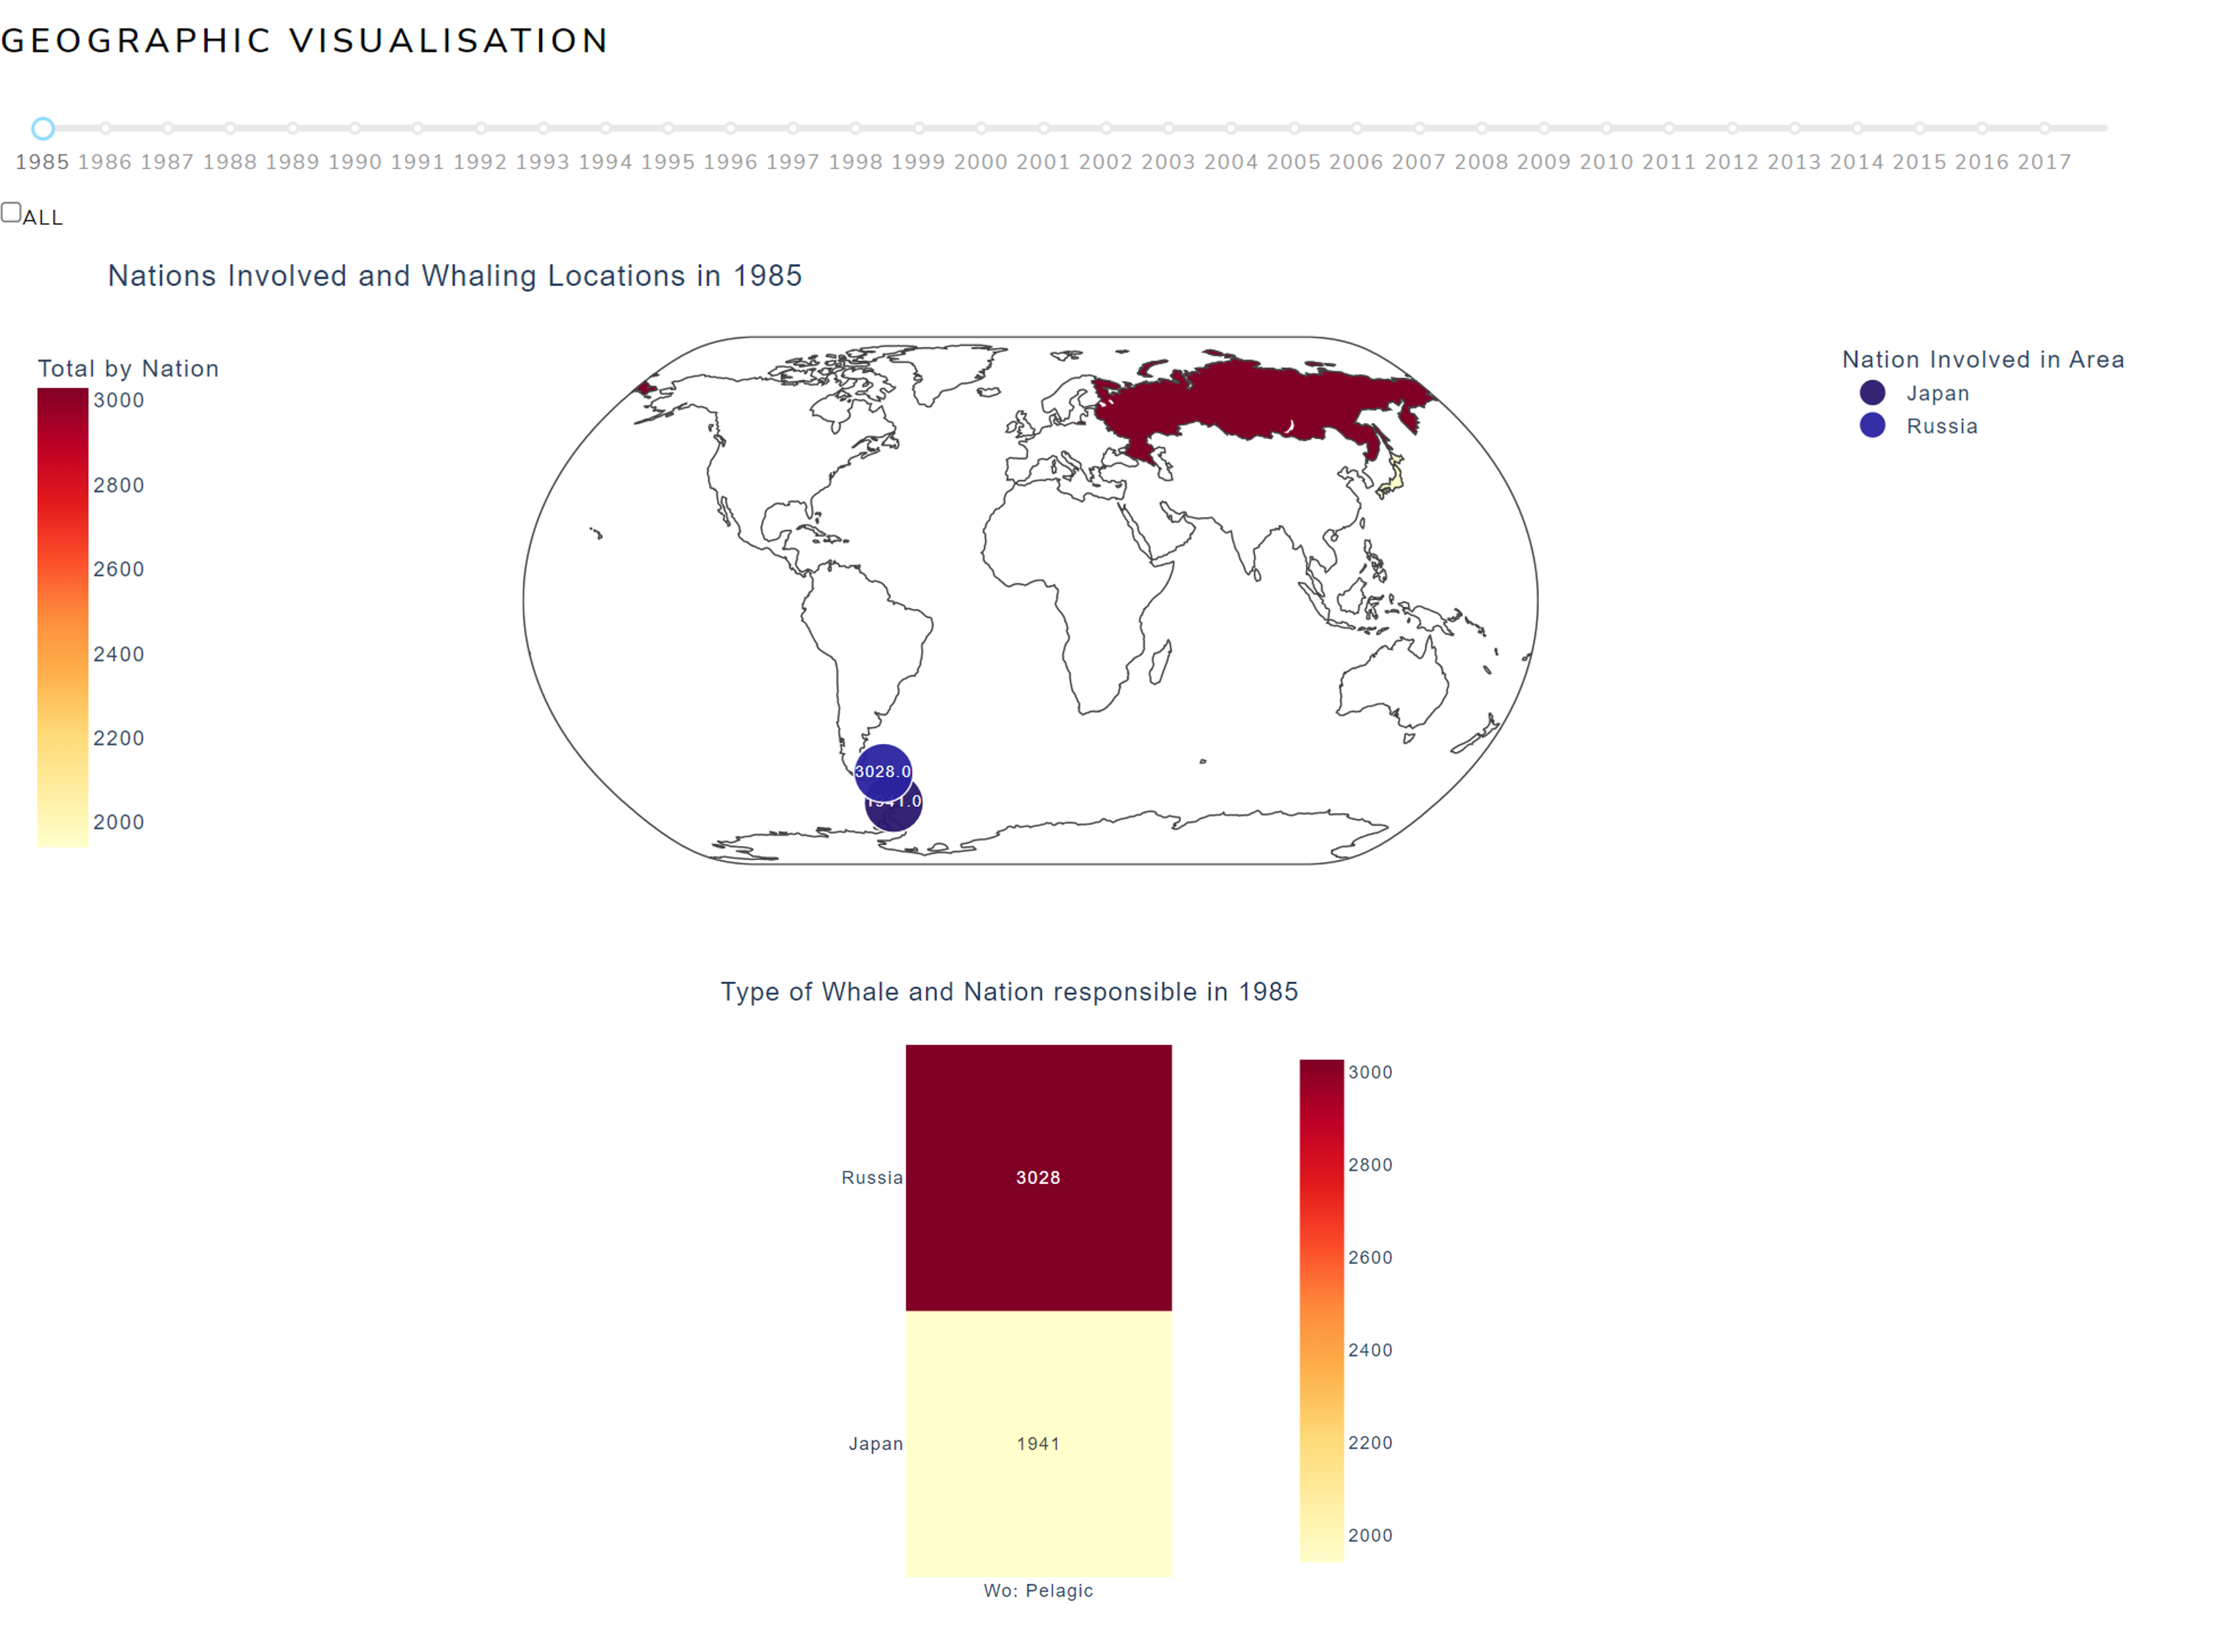
\includegraphics[width = 15cm]{Choro+corr.png}
    \caption{Geographical and Correlation Map Visualisation in year 1985}
    \label{fig:heatmap1}
\end{figure}

\begin{figure}[H]
    \centering
    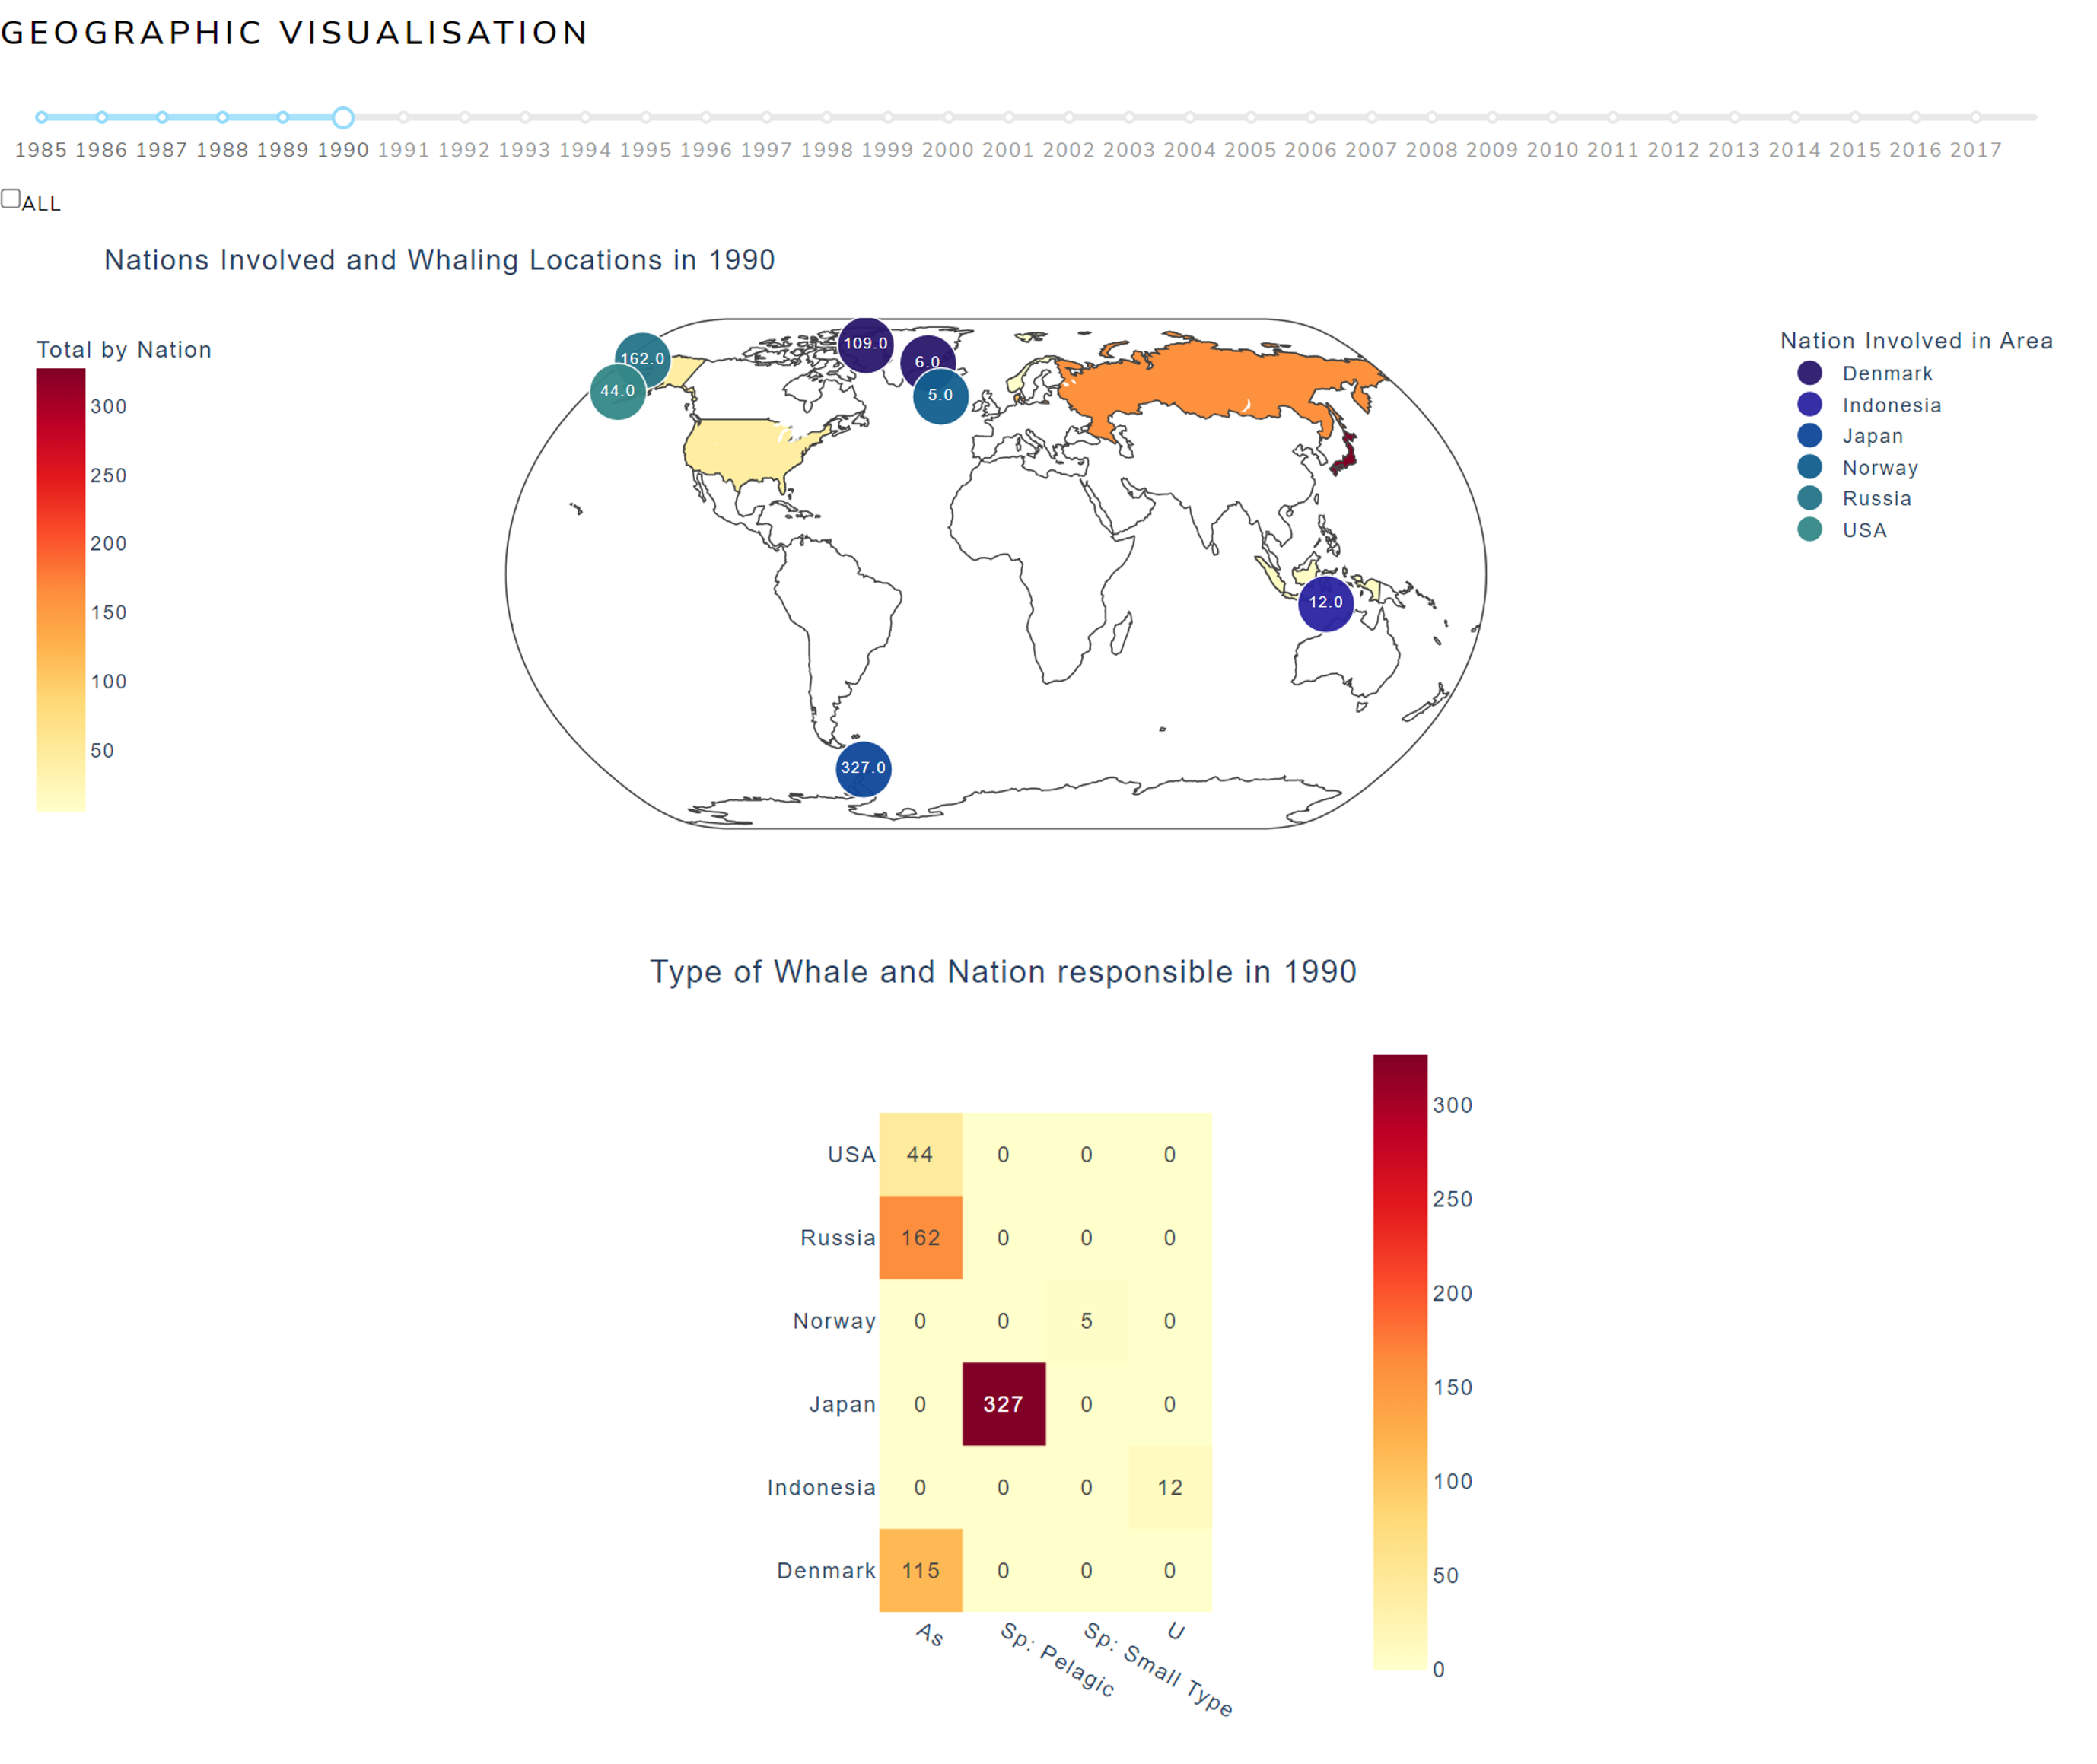
\includegraphics[width = 15cm]{Choro+corr2.png}
    \caption{Geographical and Correlation Map Visualisation in year 1990}
    \label{fig:heatmap2}
\end{figure}

\begin{figure}[H]
    \centering
    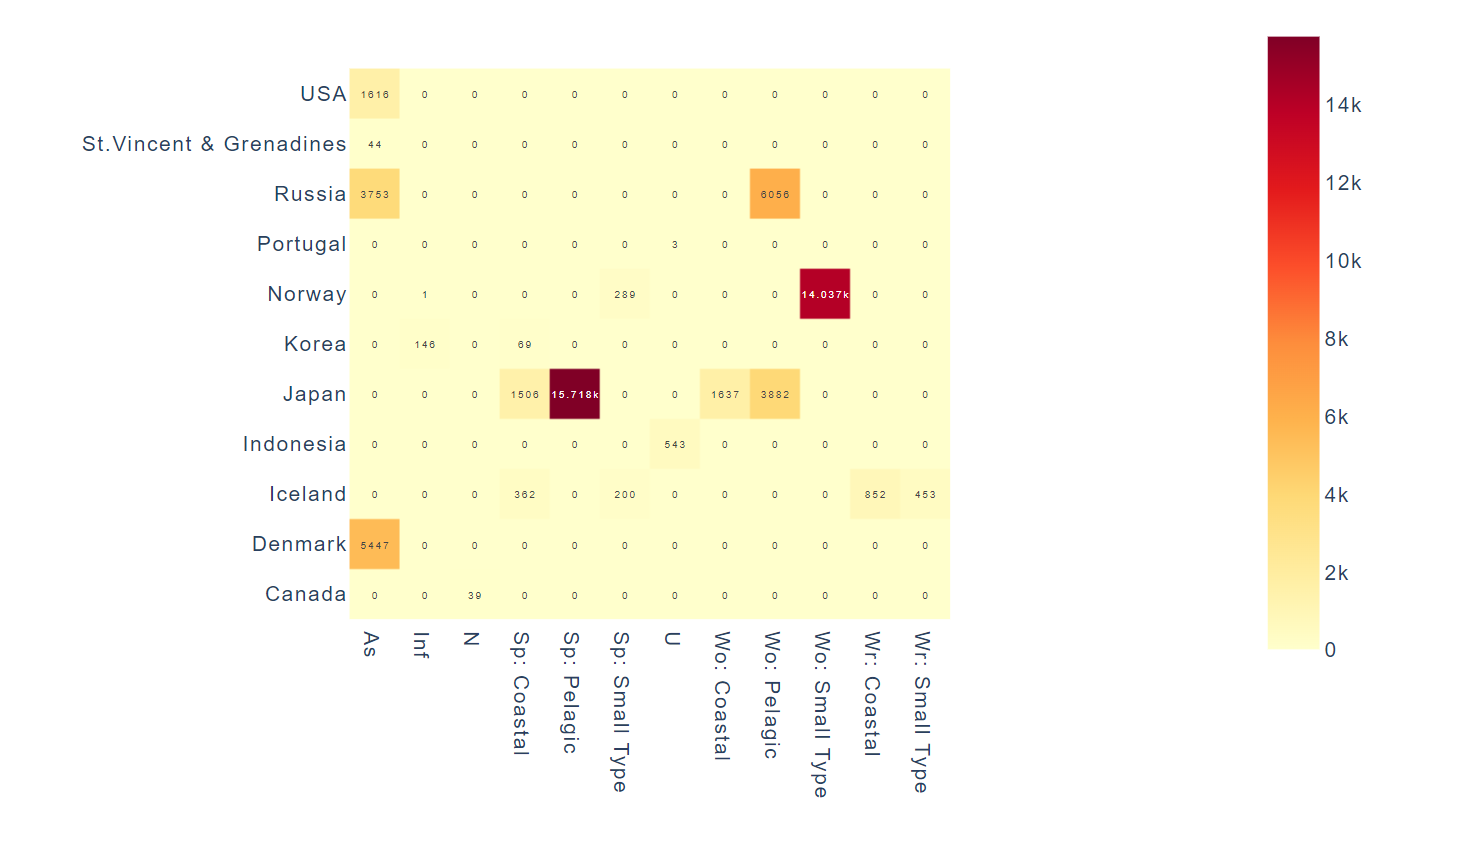
\includegraphics[width = 15cm]{heatmapALL.png}
    \caption{Geographical and Correlation Map Visualisation in year 1990}
    \label{fig:heatmapALL}
\end{figure}

\subsubsection{Evaluation}
The visualisation aids in providing a unique correlation between the type of whale, the area, and the Nation. Typically, whaling was conducted by herding whales into bay areas, as evidenced in Figure \ref{fig:heatmap2} Japan caught 327, SP: Pelagic type whales near Antartica. This may indicate that pelagic whales, which are open water whales were migrating from the south pacific region and herded towards Antarctica.Contrary most other nations 

As a result, this visualisation is useful in providing such correlations and insights into how whaling missions were conducted. 

\newpage
\subsubsection{Species and Area Correlation}
Furthermore, to provide additional granularity on the species that were targetted within a specific area, it was devised to utilise a stacked bar graph. Once again representing three-dimensional data, however as opposed to utilising a three dimensional visualisation, colour has been utilised to represent the third dimension. 

\begin{minted}[frame=single,framesep=4pt,fontsize=\small]{python}
#Horizontal Bar Graph
df_area = original_df.groupby(['Year','Area'])['Fin', 
'Sperm', 'Humpback', 'Sei', 'Bryde\'s', 'Minke', 'Gray', 'Bowhead'].sum().reset_index()

df_area_total = original_df.groupby(['Area'])['Fin', 
'Sperm', 'Humpback', 'Sei', 'Bryde\'s', 'Minke', 'Gray', 'Bowhead'].sum().reset_index()
\end{minted}

\begin{figure}[H]
    \centering
    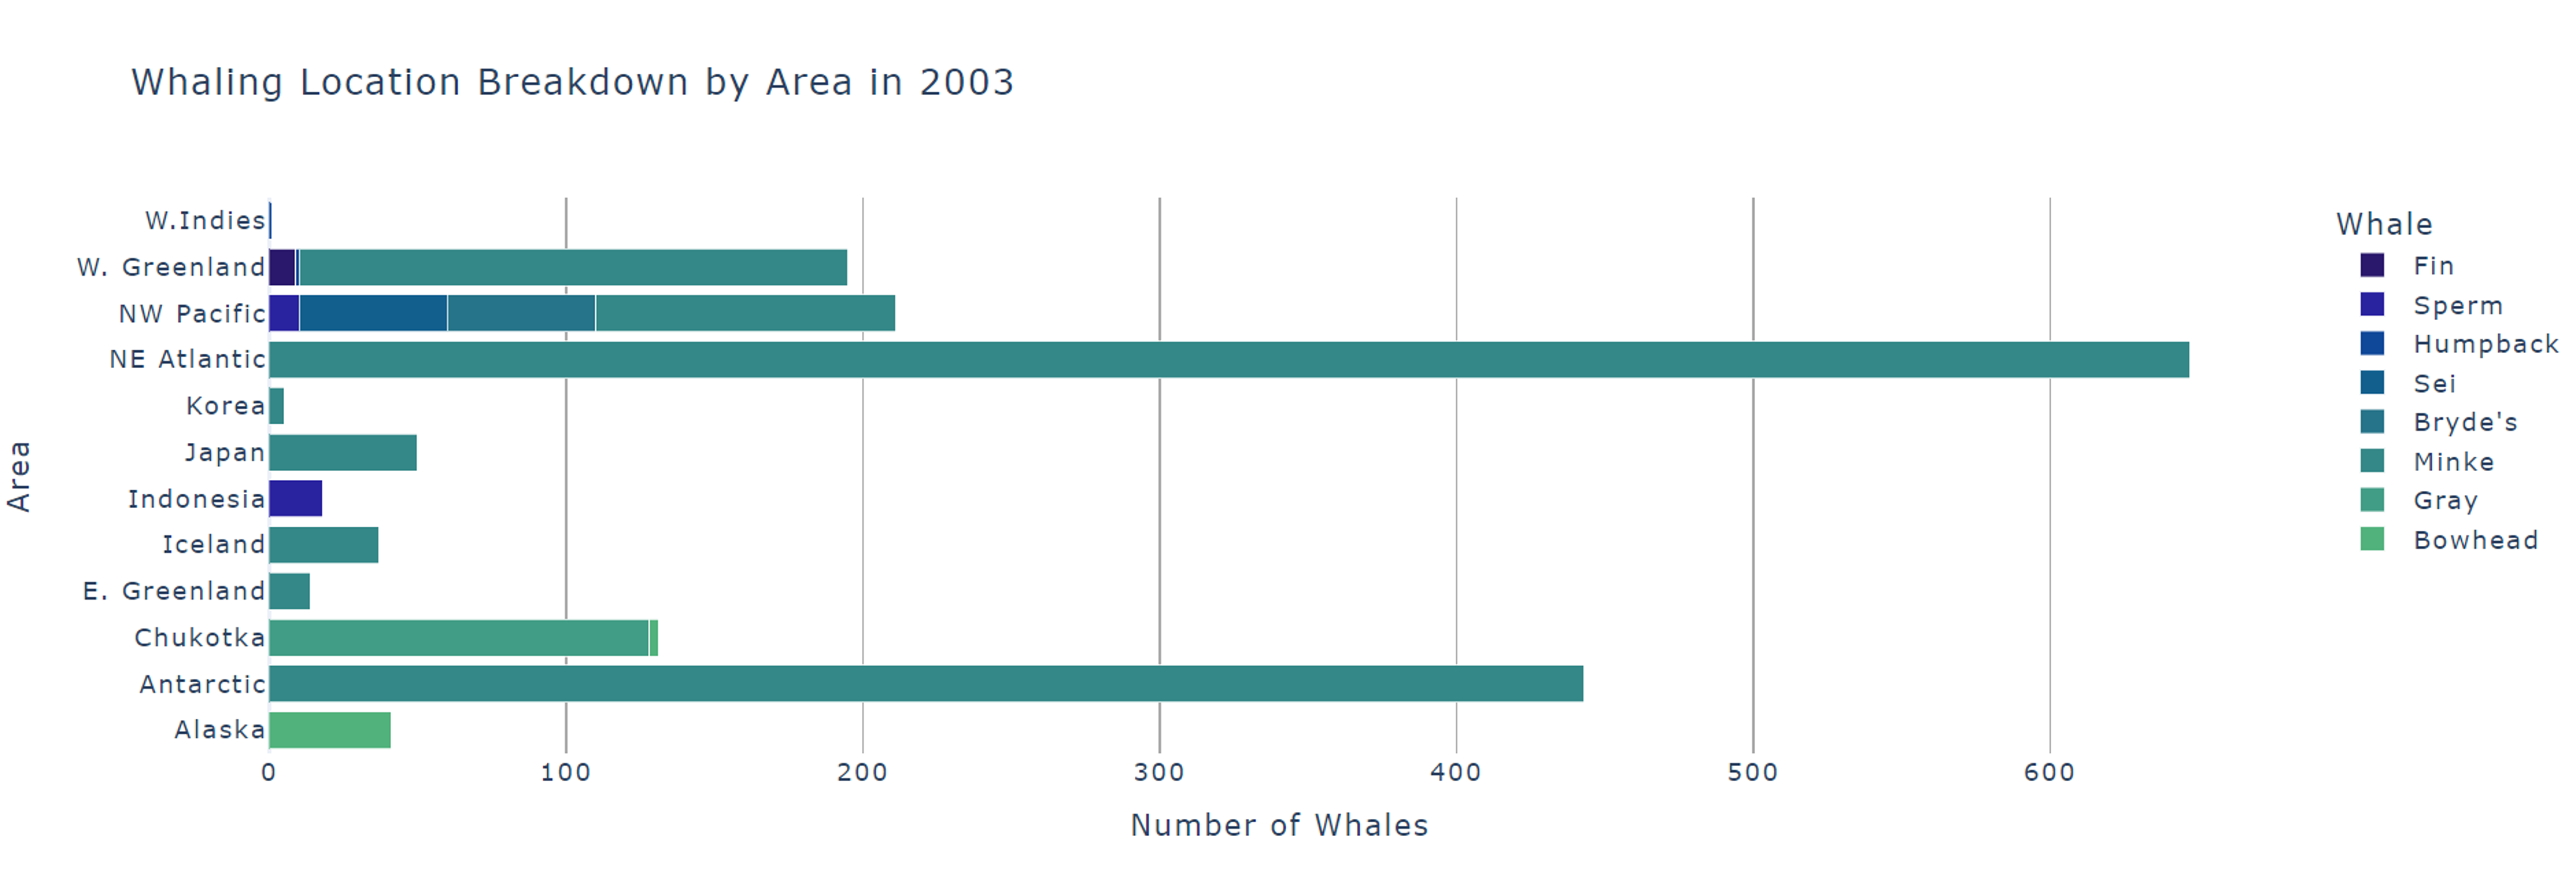
\includegraphics[width = 15cm]{horizontalBarNolog.png}
    \caption{Initial Species and Area breakdown visualisation in year 2003}
    \label{fig:my_label}
\end{figure}
From the above initial visualisation it was evaluated that the typical scale made it difficult to observe all bar values. Thus, utilising a logarithmic x axis scale was utilised. 

\begin{figure}[H]
    \centering
    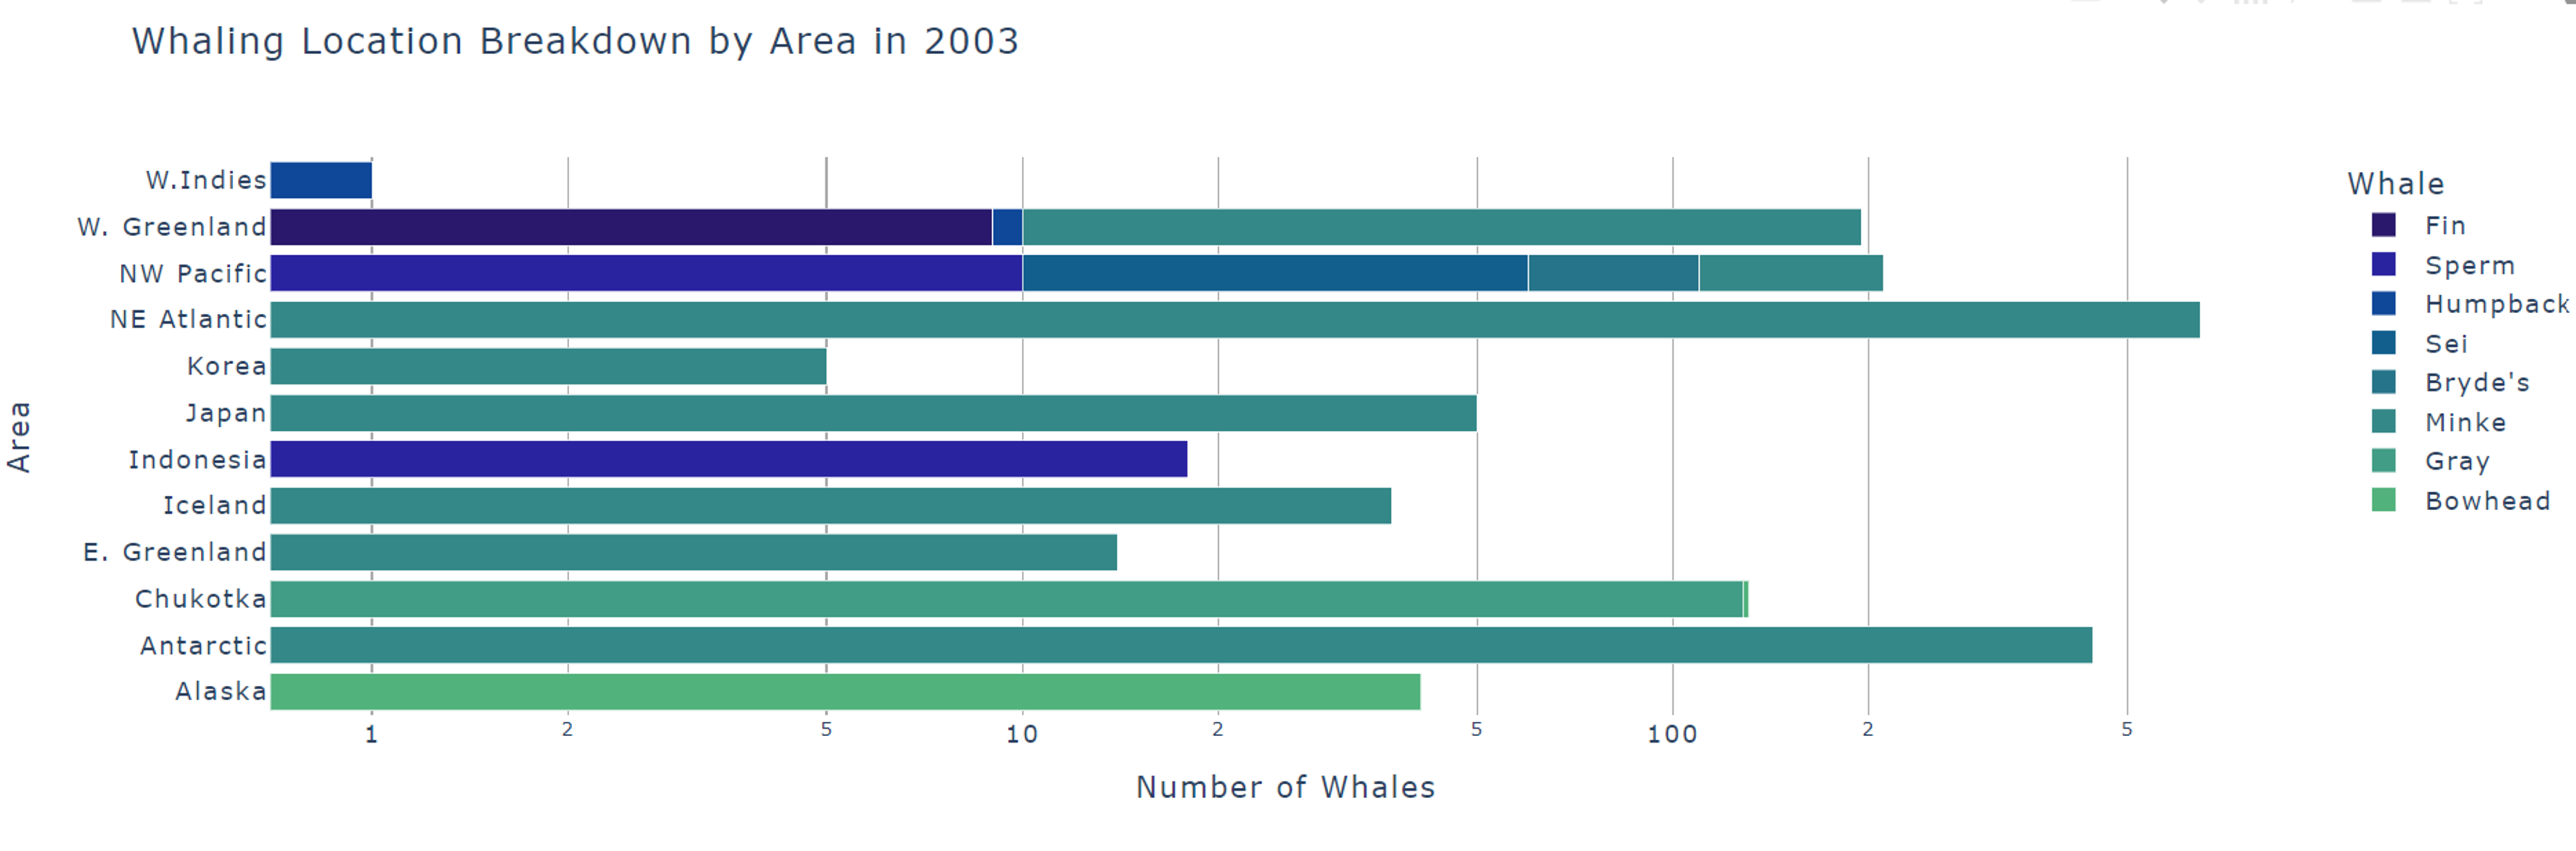
\includegraphics[width = 15cm]{horizontalBarLog.png}
    \caption{Final Species and Area breakdown visualisation in year 2003}
    \label{fig:my_label}
\end{figure}

\subsubsection{Evaluation}
The above visualisation was effective in assisting the geographic visualisation and further complements the  Type and Nation correlation keymap. This was observed as each area can be deduced on the choropleth map, where the colour legend implies which Nation was involved. This provides insights, into which nation contributed to the loss of the respective species within the area. Moreover, this can then be correlated to the correlation keymap, which provides insight into what 'Type' category the following species within that area would fall into. 


Furthermore, it can be observed using the cumulatative variation of all charts that the most affected species across all areas was the Minke whale population. Additoinally, the area that had the highest catch numbers was reportedly in Antartica, where Nations Japan and Russia, were primarily involved. 

Other interesting findings from these visualisations include, Humpback whales primarily caught near the West Indies region, by St Vincent and Grenandines. Along with the most diverse species distribution of whales found off the coast of Alaska. These whales were primarily caught by the United States. These whales however were all classified as AS Type whales. 



\subsection{Categorical Visualisation}
Whilst the above set of multivariate data visualisations were succesful in providing a holistic overview on the data's feature sets.
It may be more preferrable to try and condense this visualisation into a single visualisation. Due to the nature of the data's dimensions primarily being labelled, categorical data and discrete data, the data can be hierachially clustered. This is provides a much more comprehensive visualisation in comparison to other multi-dimensional visualisations such as three-dimensional scatter plots which is much better suited for continuous data. 

 The first group, within the hierarchy, was devised as the Nation, followed by the Species, and then using a stacked bar to represent the Type variation. A logarithmic scale was once again utilised to assist with the readability of the visualisation. The interactive slider bar feature has been included once again to allow the viewer to observe values across each point in time. Along with the 'ALL' checkbox feature which provides a cumulative total across all years. 
\begin{minted}[frame=single,framesep=4pt,fontsize=\small]{python}
 original_df['CODE']=alpha3code(original_df['Nation'])

stacked = original_df.groupby(['Year','CODE', 'Type'])
['Fin', 'Sperm', 'Humpback', 'Sei', 'Bryde\'s', 'Minke',
'Gray', 'Bowhead'].sum().reset_index()

stacked_total = original_df.groupby(['CODE', 'Type'])['Fin',
'Sperm', 'Humpback', 'Sei', 'Bryde\'s', 'Minke', 'Gray', 
'Bowhead'].sum().reset_index()
\end{minted}
\begin{figure}[H]
    \centering
    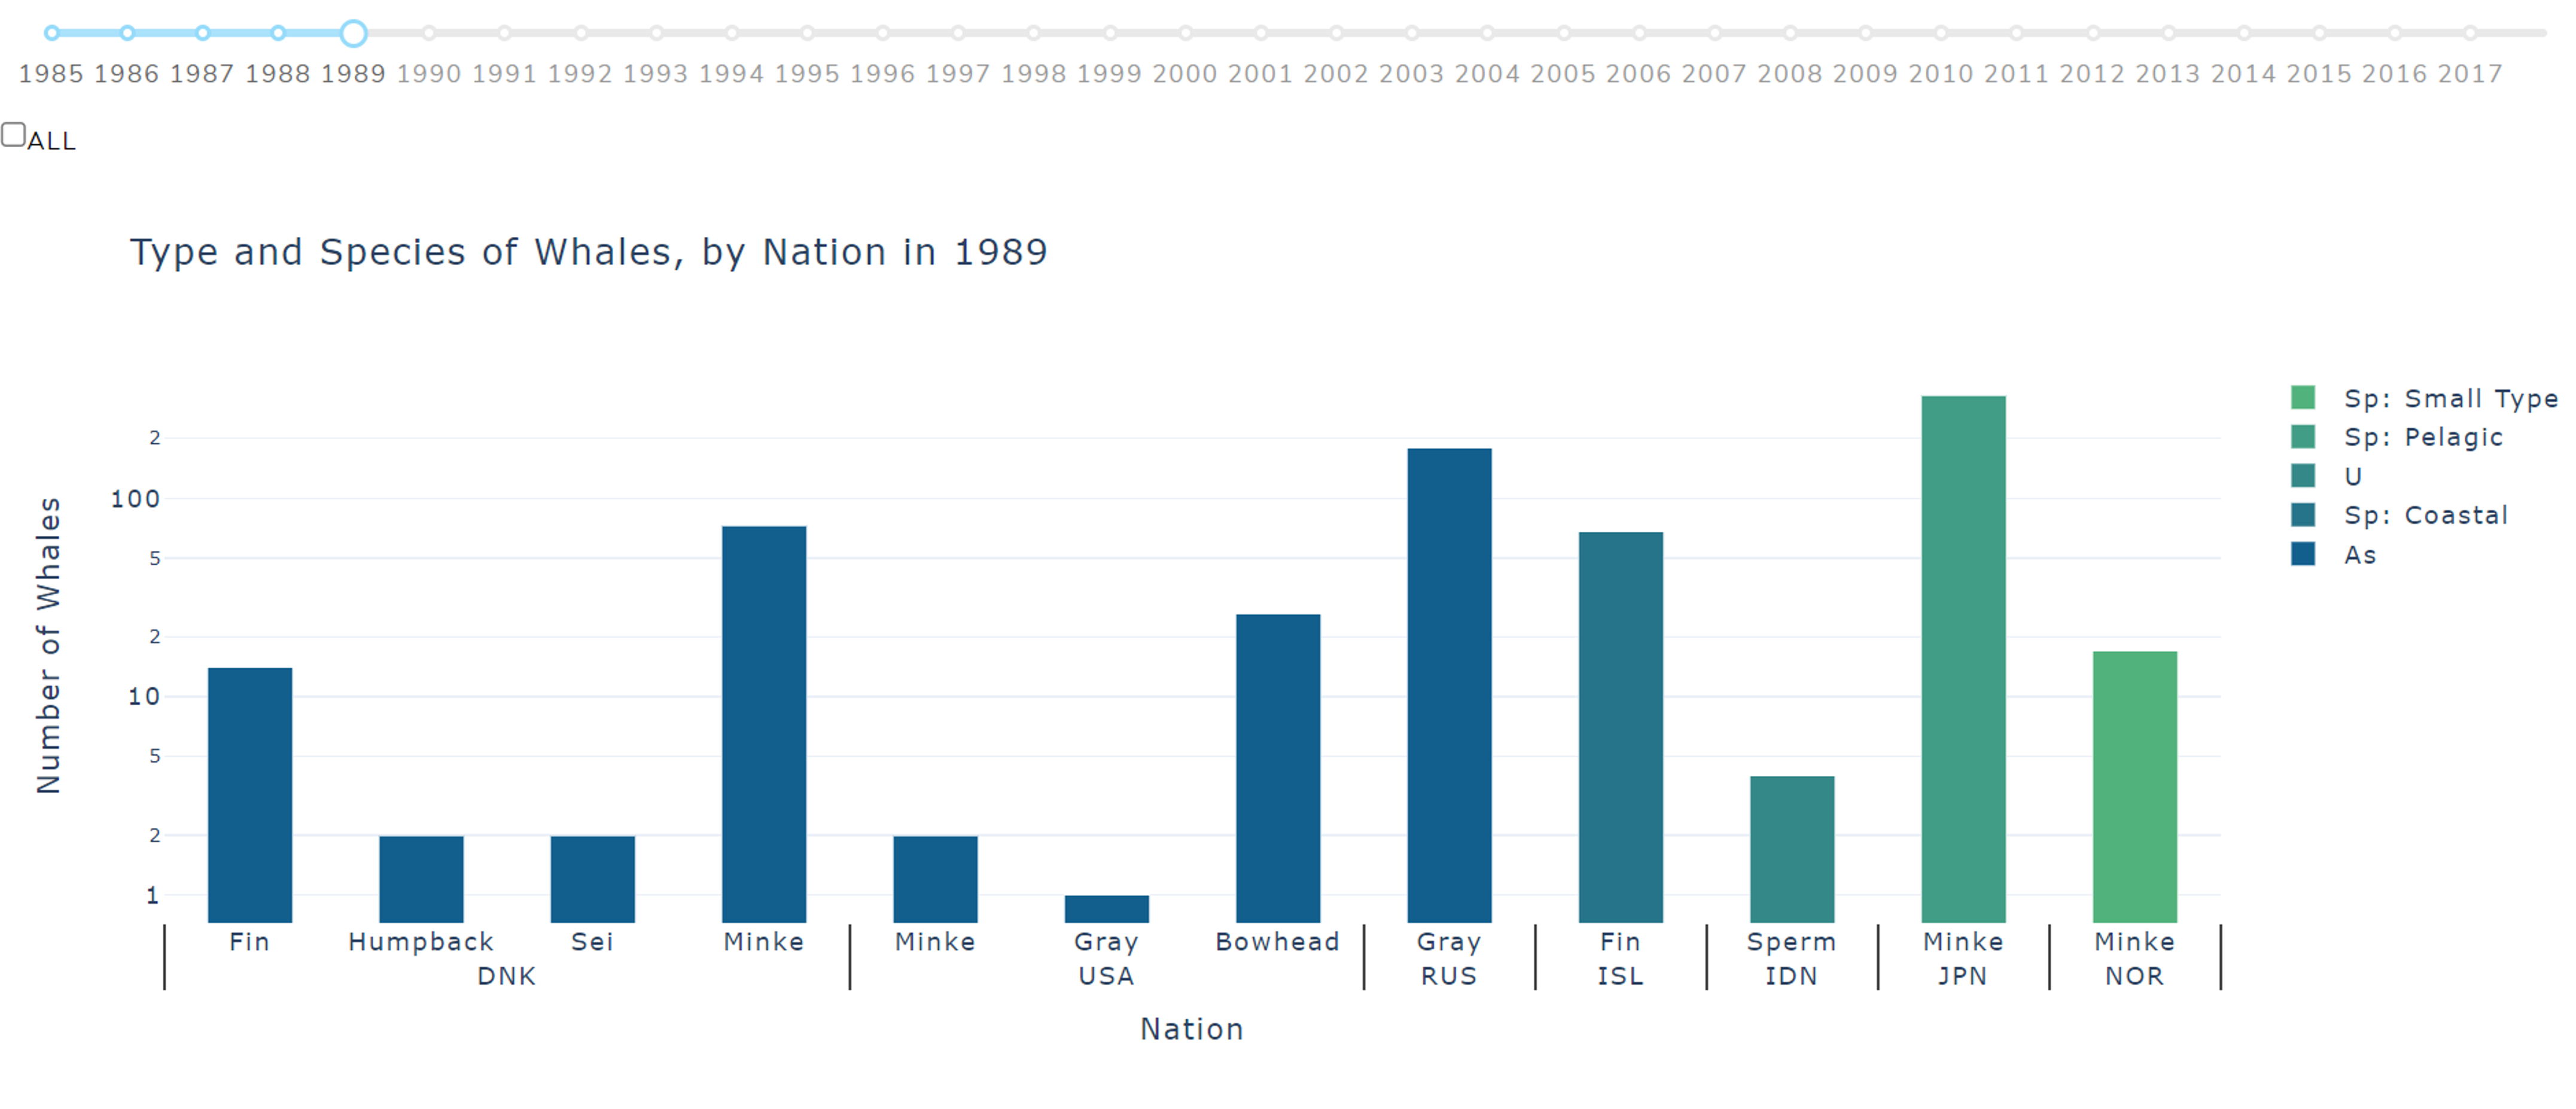
\includegraphics[width = 15cm]{Categorical.png}
    \caption{Clustered and Stacked Bar Plot of Species, Type and Nation by Year}
    \label{fig:my_label}
\end{figure}


\begin{figure}[H]
    \centering
    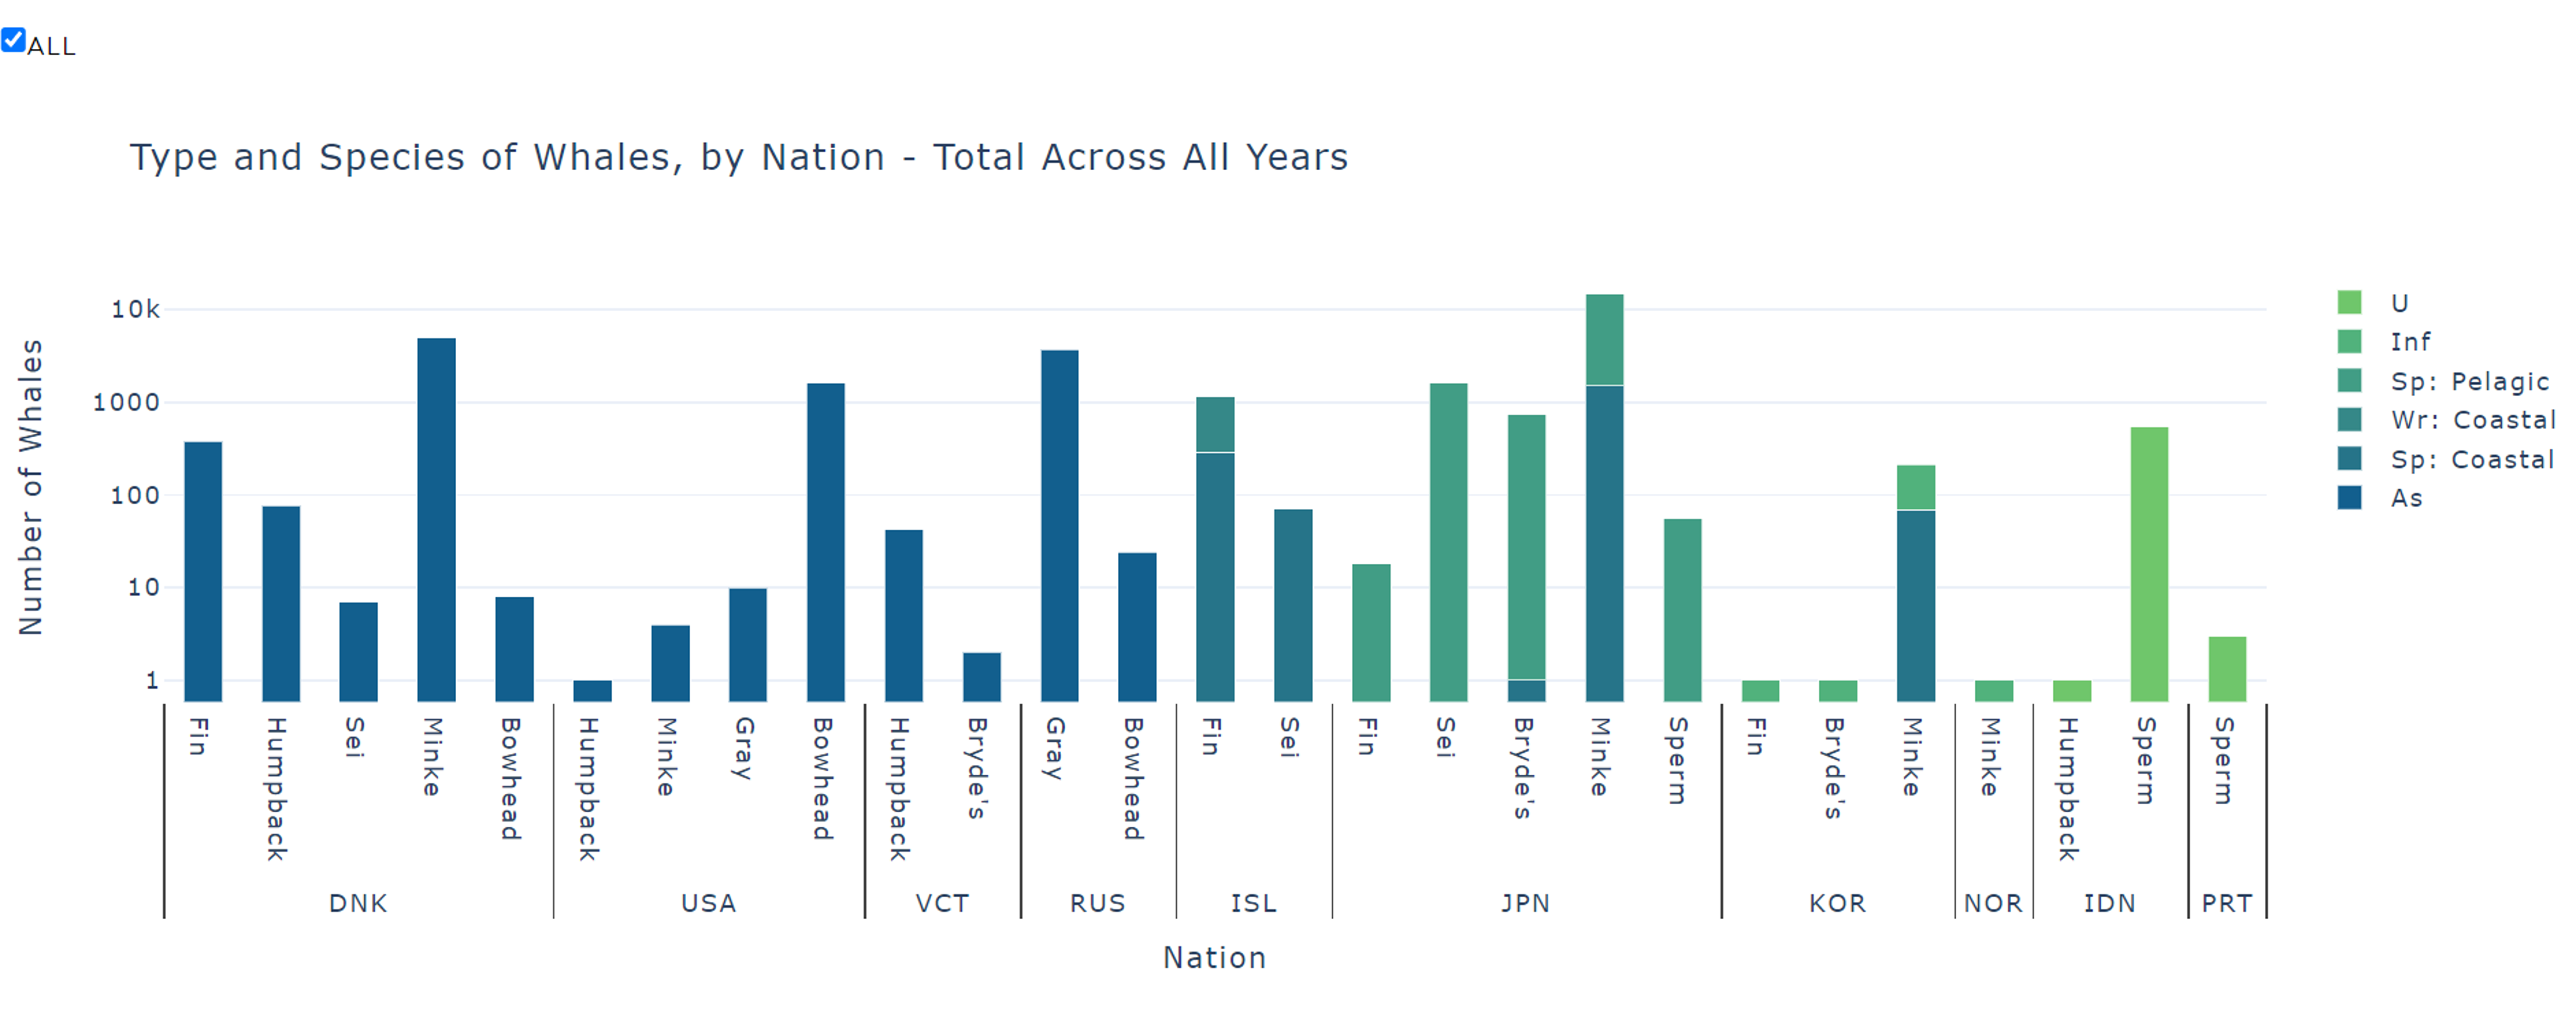
\includegraphics[width = 15cm]{CategoricalALL.png}
    \caption{Clustered and Stacked Bar Plot of Species, Type and Nation across all years}
    \label{fig:my_label}
\end{figure}


\subsubsection{Evaluation}
The visualisation provides a much more concise overview on three of the feature sets although unlike the previous visualisation doesn't attain information about the geographical locations. Whilst this dimension could have been included, it made the visualisation too complex to interpret. Nonetheless, the visualisation contains vital information such as highlighting how the 'AS' classification contains a wide distribution of species. Along with Denmark and Japan obtaining the largest range of catch species, in comparison to Norway and Indonesia where only selective whale species were caught. 



\subsection{Time-series Visualisation}
The prior visualisations primarily focused on the values at particular points in time and the various correlations between feature sets. However, the data can be grouped into a bivariate form, with time as the independent variable, observing the aggregate total as the dependent variable. Thereby incorporating the time-series nature of the data which is best represented by using a scatter plot or line graph. 
Additionally, such a visualisation would be more informative, if the aggregate trends between various features could be compared. As a result, adding an added dimensionality deducing the visualisation as multivariate. It was devised that observing each Nations whaling activities over time would provide a piece of more constructive information on the trajectory of commericial whaling. 
\begin{minted}[frame=single,framesep=4pt,fontsize=\small]{python}
#Time Series Data
df = original_df.groupby(['Year','Nation'])
['Total'].sum().reset_index()
\end{minted}

\begin{figure}[H]
    \centering
    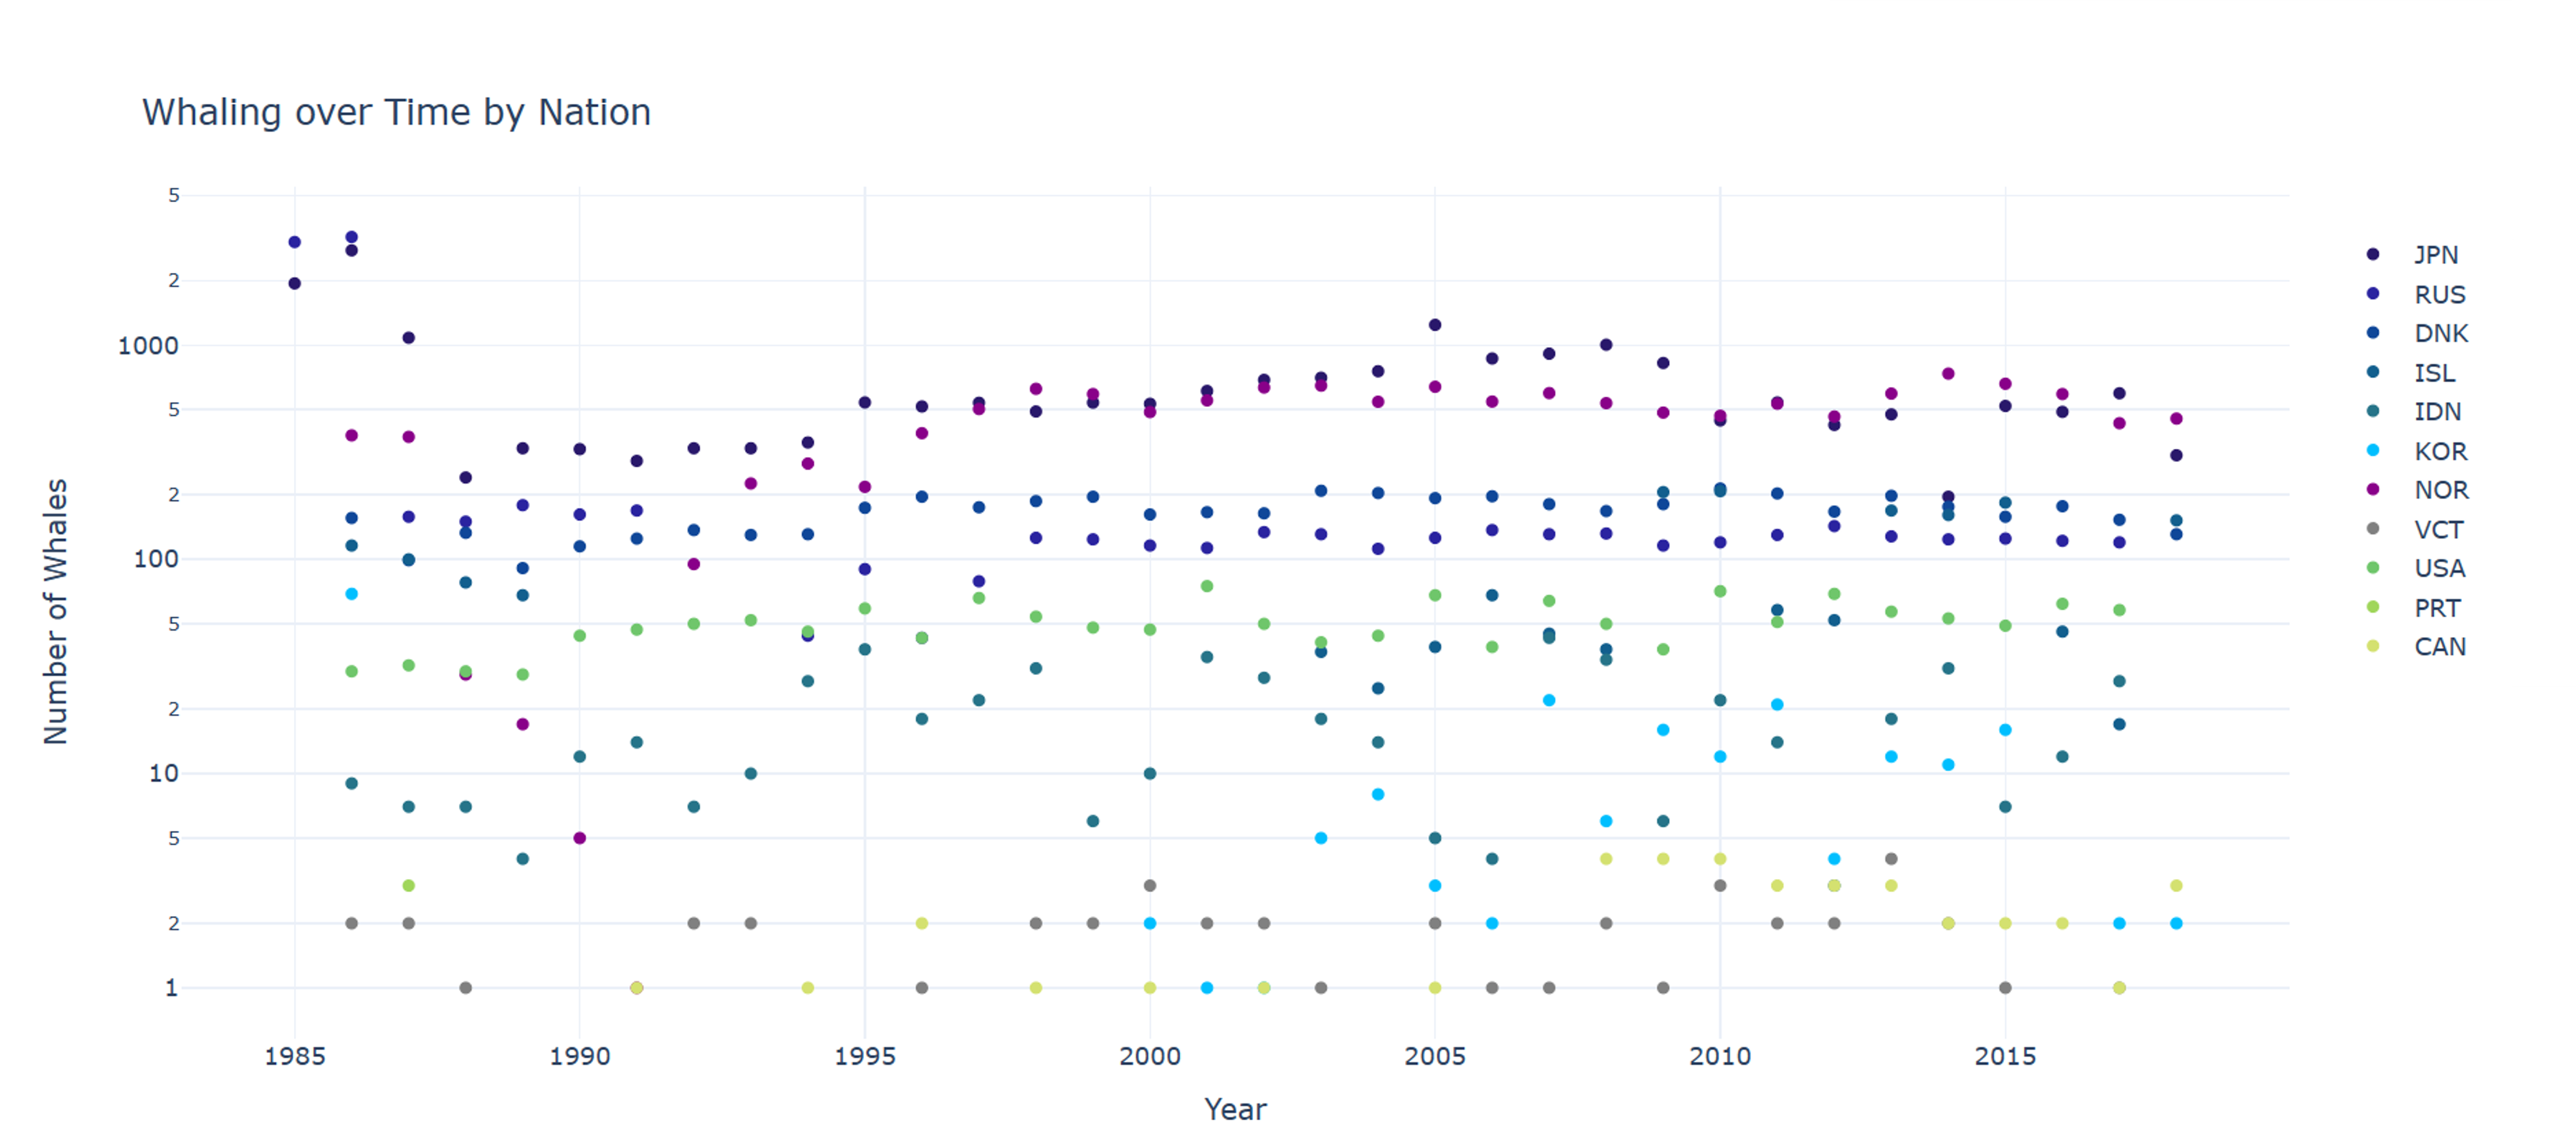
\includegraphics[width = 15cm]{AllScatter.png}
    \caption{Final Species and Area breakdown visualisation in year 2003}
    \label{fig:my_label}
\end{figure}

Upon initial observations of the above scatter plot, it is evident that it is very difficult to deduce any sort of information fromt his figure with 11 different data labels and trend distributions. Moreover, there doesn't appear to be any form of clustering or clear cyclical behavior. 

As a result, in order to further assist readability, an interactive check box feature was included, allowing the viewer to select each Nation's trend distribution. Moreover, as the data is particularly volatile various curve-smoothing and fit methods were explored. 

The final curve-fit technique utilised was the Locally weighted scatterplot smoothing, method. This method applies non-linear regression analysis and provides a means to decrease the voltatility in the data series, making the trend much more observable. Furthermore, the LOWESS regression method obtains a tuning parameter known as a fraction parameter. This parameter assists in controlling the smoothness of the curve. The standard value of this is 0.666, however, the respective curve smoothing factors have been applied for the following Nations. 

\begin{table}[H]
\rowcolors[]{1}{white}{teal!10}
\centering
\begin{tabular}{| m{5cm} |m{10cm}|}
\hline
 \textbf{Nation} & \textbf{LOWESS Fraction Parameter}\\ 
 \hline
    JPN & 0.46\\ 
\hline
    NOR & 0.28\\ 
\hline
    RUS & 0.23\\ 
\hline
    Every other nation & 0.666\\ 
\hline
\end{tabular}
 \caption{\label{tab:table1} Various LOWESS Fraction Parameters}
\end{table}

\begin{figure}[H]
    \centering
    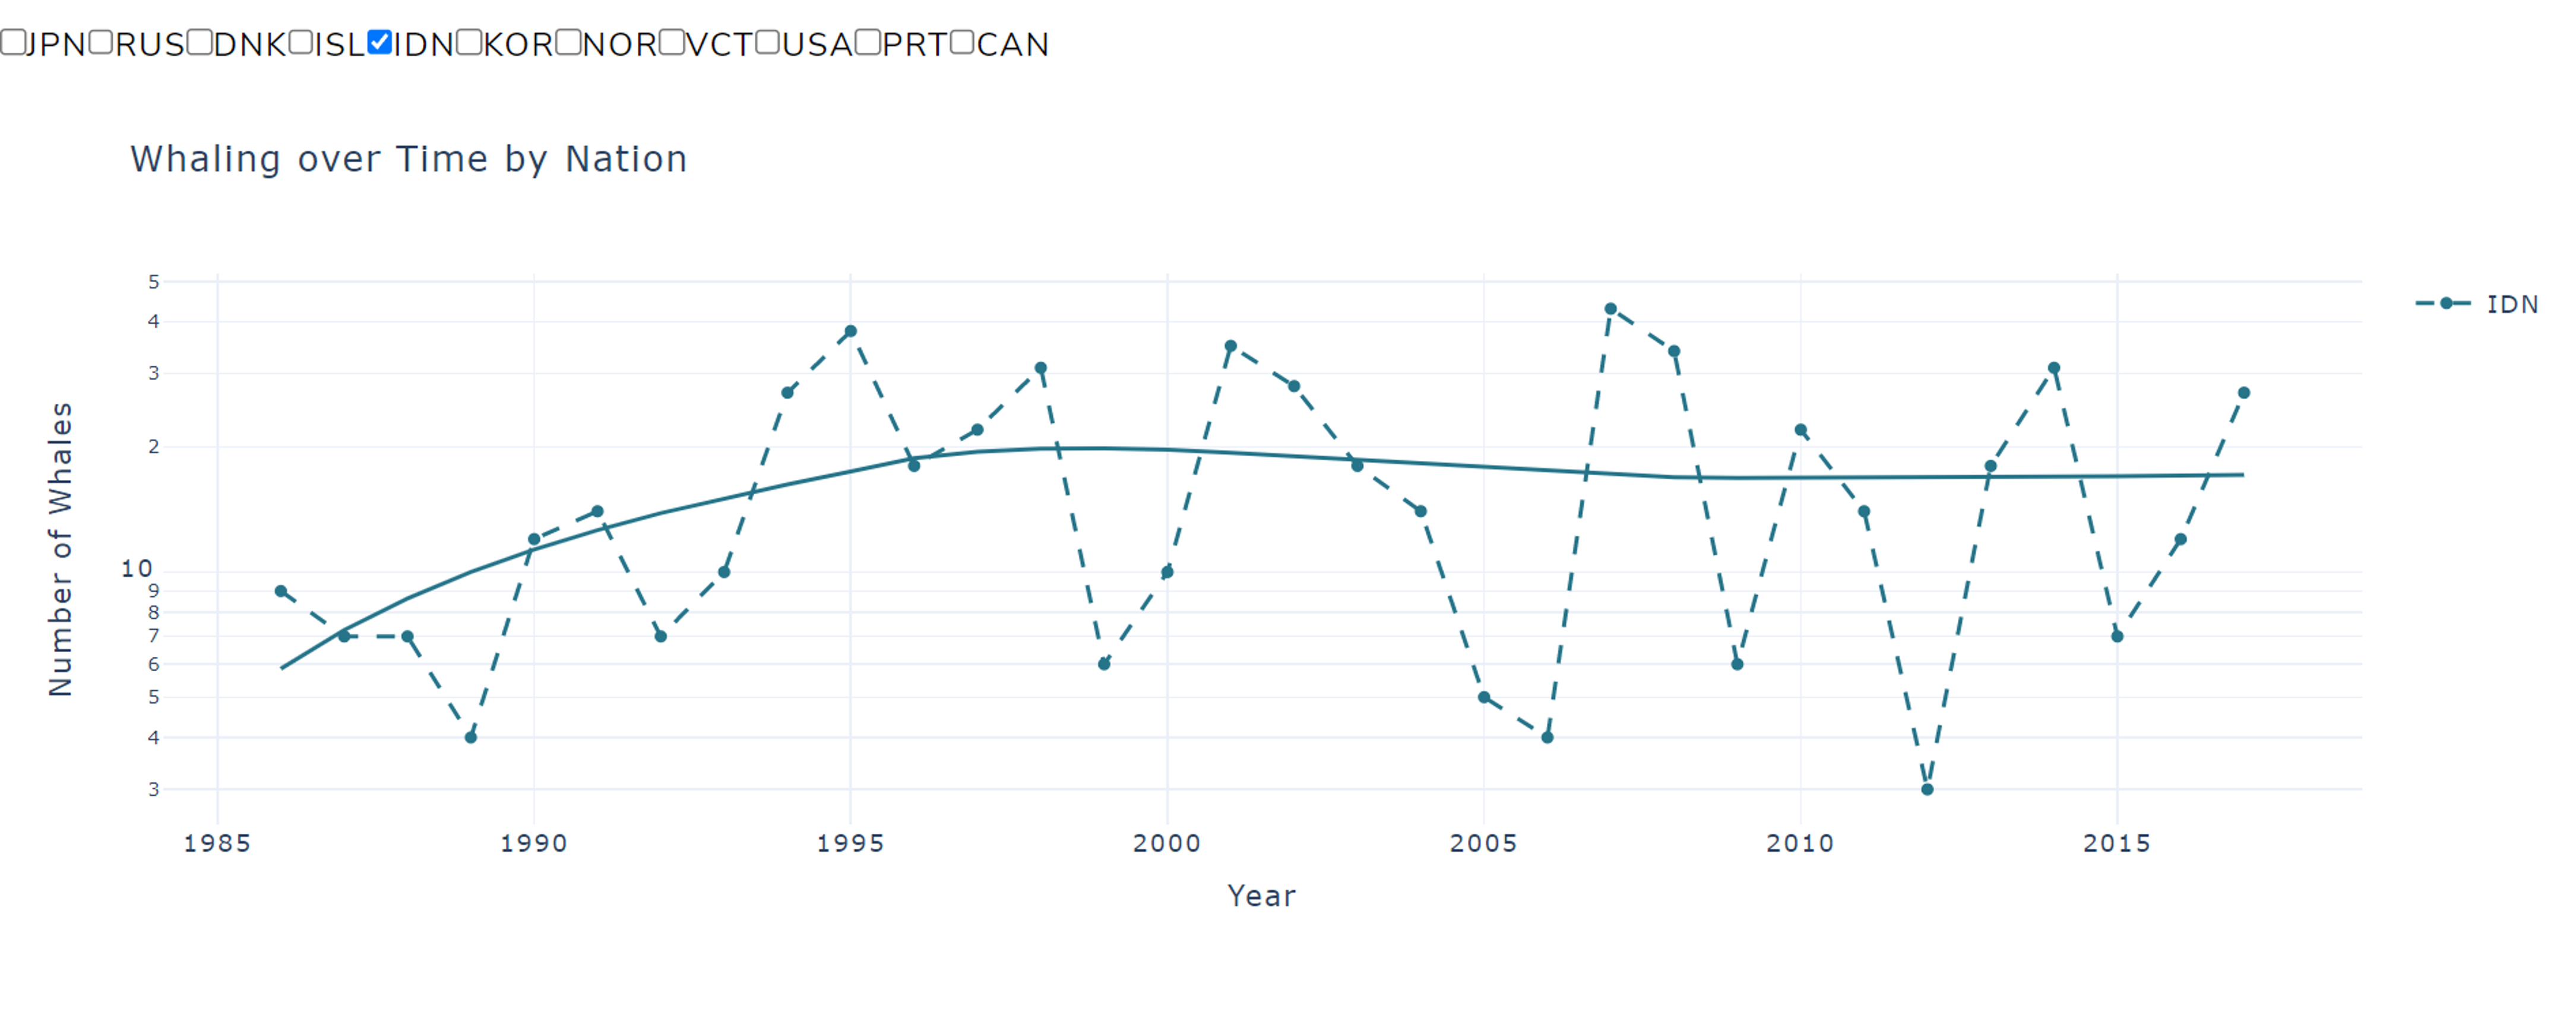
\includegraphics[width = 15cm]{SingleTrend.png}
    \caption{Final Time Series Visualisation of Indonesia (Bivariate)}
    \label{fig:my_label}
\end{figure}



\begin{figure}[H]
    \centering
    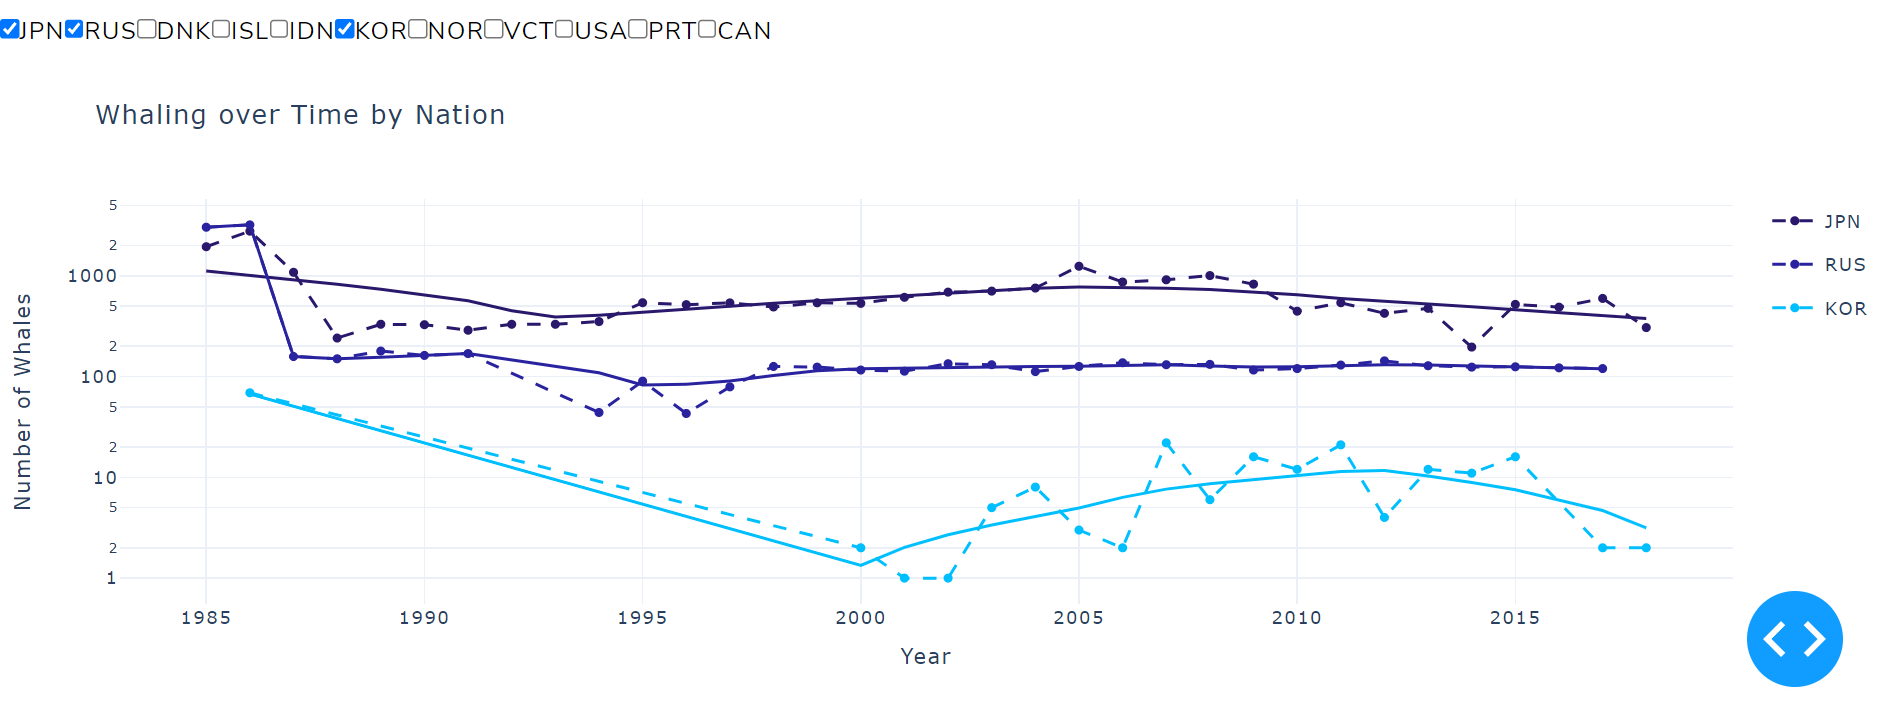
\includegraphics[width = 15cm]{MultiVariateTrend.png}
    \caption{Final Time Series Visualisation of Japan, Russia and Korea (Multivariate)}
    \label{fig:my_label}
\end{figure}

 


\subsubsection{Evaluation}
 The time series visualisation whilst simple, provides crucial information on the long-term trend of commercial whaling. 
 
 An overall observation for all trend lines suggests that each Nation appears to stay within a particular range of values, however within the initial decade from 1980 to 1990 catches were much more volatile.  Nonetheless, over time, most Nation's catches seem to be either in decline or modulating between the same range of values. 

 
 Additionally, provided the assistance of the clustered visualisation, each year data point can be made more granular by observing the countries species and type break down at that particular point in time. As a result, these two visualisations complement one another. 


\subsection{Data Blending Visualisation}
Data Blending involves combining data from multiple sources into a functioning dataset.  (Reference) This was undertaken to better represent the impact of whaling on each species, by integrating the IUCN Red List of Threatened Cetacean Species data set.  This was accomplished by creating a dictionary 'decades\_dict' which stored keys corresponding to aggregate data of commercial whaling dataset across each decade (Refer to Appendix X), then mapping corresponding Red List label, for each species. The data was then represented using a polar bar graph, which is an effective means of comparing categorical or continuous data and observing cyclical behavior.

\begin{minted}[frame=single,framesep=4pt,fontsize=\small]{python}
#IUCN Redlist and Whaling data set blend. 
#polarPlot.decades_dict created in separate file 

data = pd.read_csv('Project\\EndangeredLists.csv')
df_endanger= pd.DataFrame(data)

keys = list(polarPlot.decades_dict[decade].keys())
decade_dataFrame['Nation'] = keys

#Collapse individual species columns into a single column
decadeMelted = pd.melt(decade_dataFrame, id_vars=['Nation'], var_name='Whale')
decadeMelted = decadeMelted.sort_values('Nation')

#Mapping of Species into decade dataframe for each 'Whale' species
decadeMelted['RedList'] = decadeMelted['Whale'].map(df_endanger.set_index('Species')
[decade])
\end{minted}


Upon combining the data set, it was devised that the most effective representation would be to utilise the angular axes as a categorical label for each Nation, with the radial values as the number of whales caught, within the prescribed Red List label category. To then analyse any repetitve or cyclical behaviour, three plots would be provided across each decade. Whilst an interactive slider could also be utilised, the visualisation was found to be much more effective when provided the ability to easily compare across each decade. 


\begin{figure}[H]
    \centering
    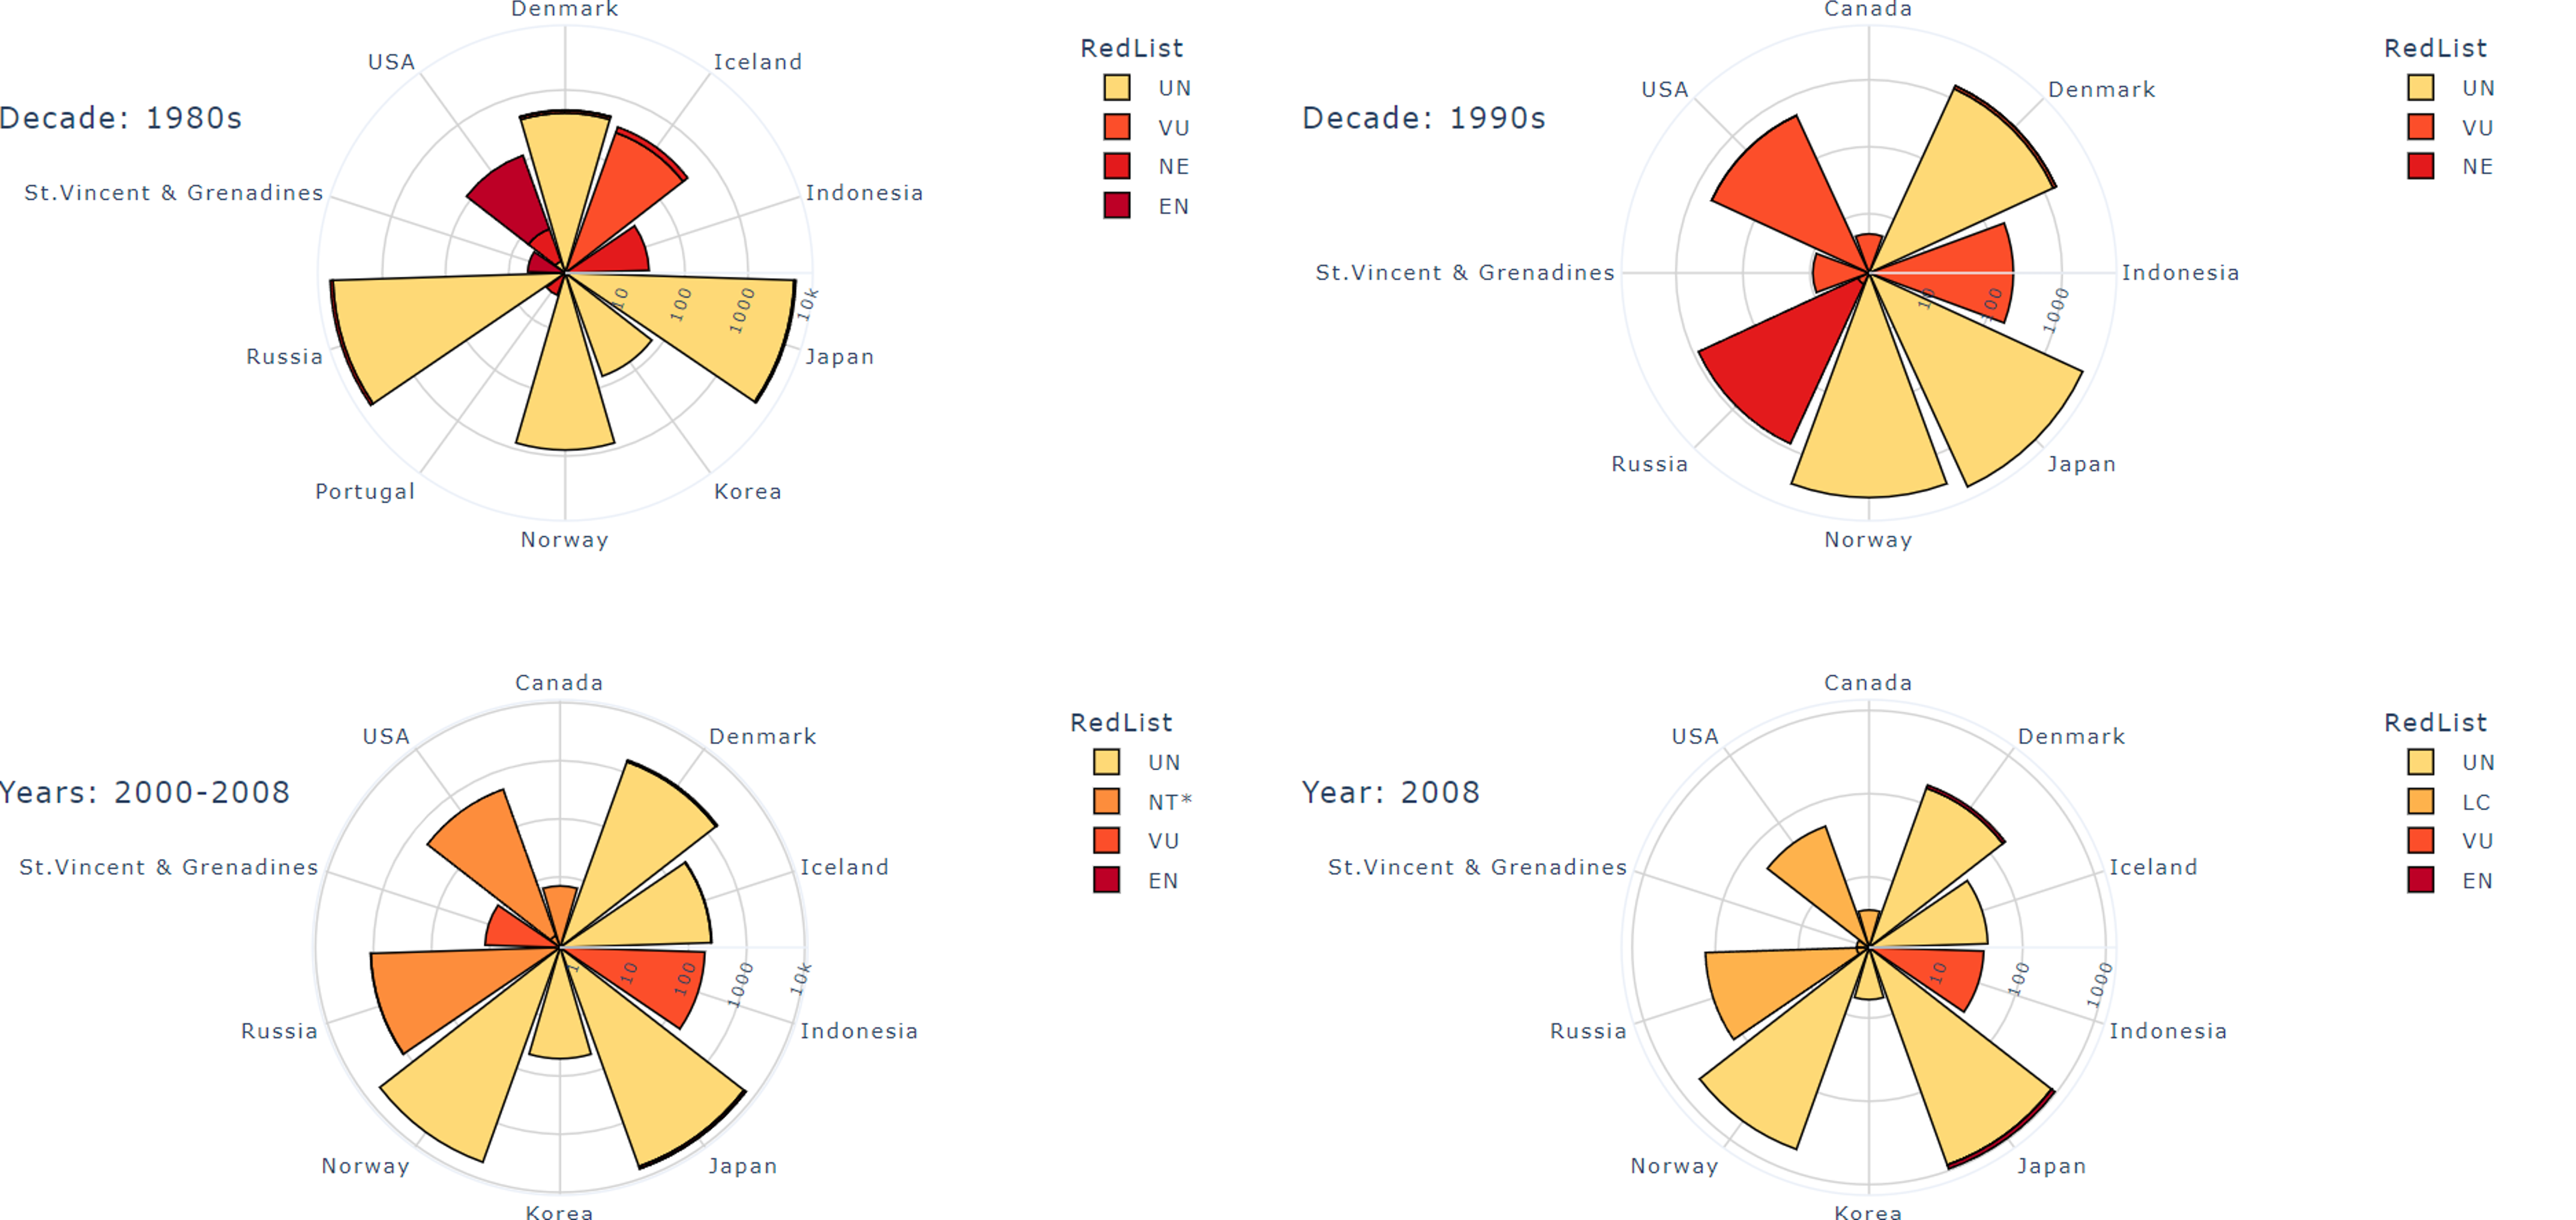
\includegraphics[width = 18cm]{polarGraph.png}
    \caption{Final Species and Area breakdown visualisation in year 2003}
    \label{fig:my_label}
\end{figure}

Additional features of this visualisation include the ability to select and remove legend attributes, along with hover text providing information on the species. This aids in deducing which Nations were potentially responsible for the endangerment of a particular species. 

\begin{figure}[H]
    \centering
    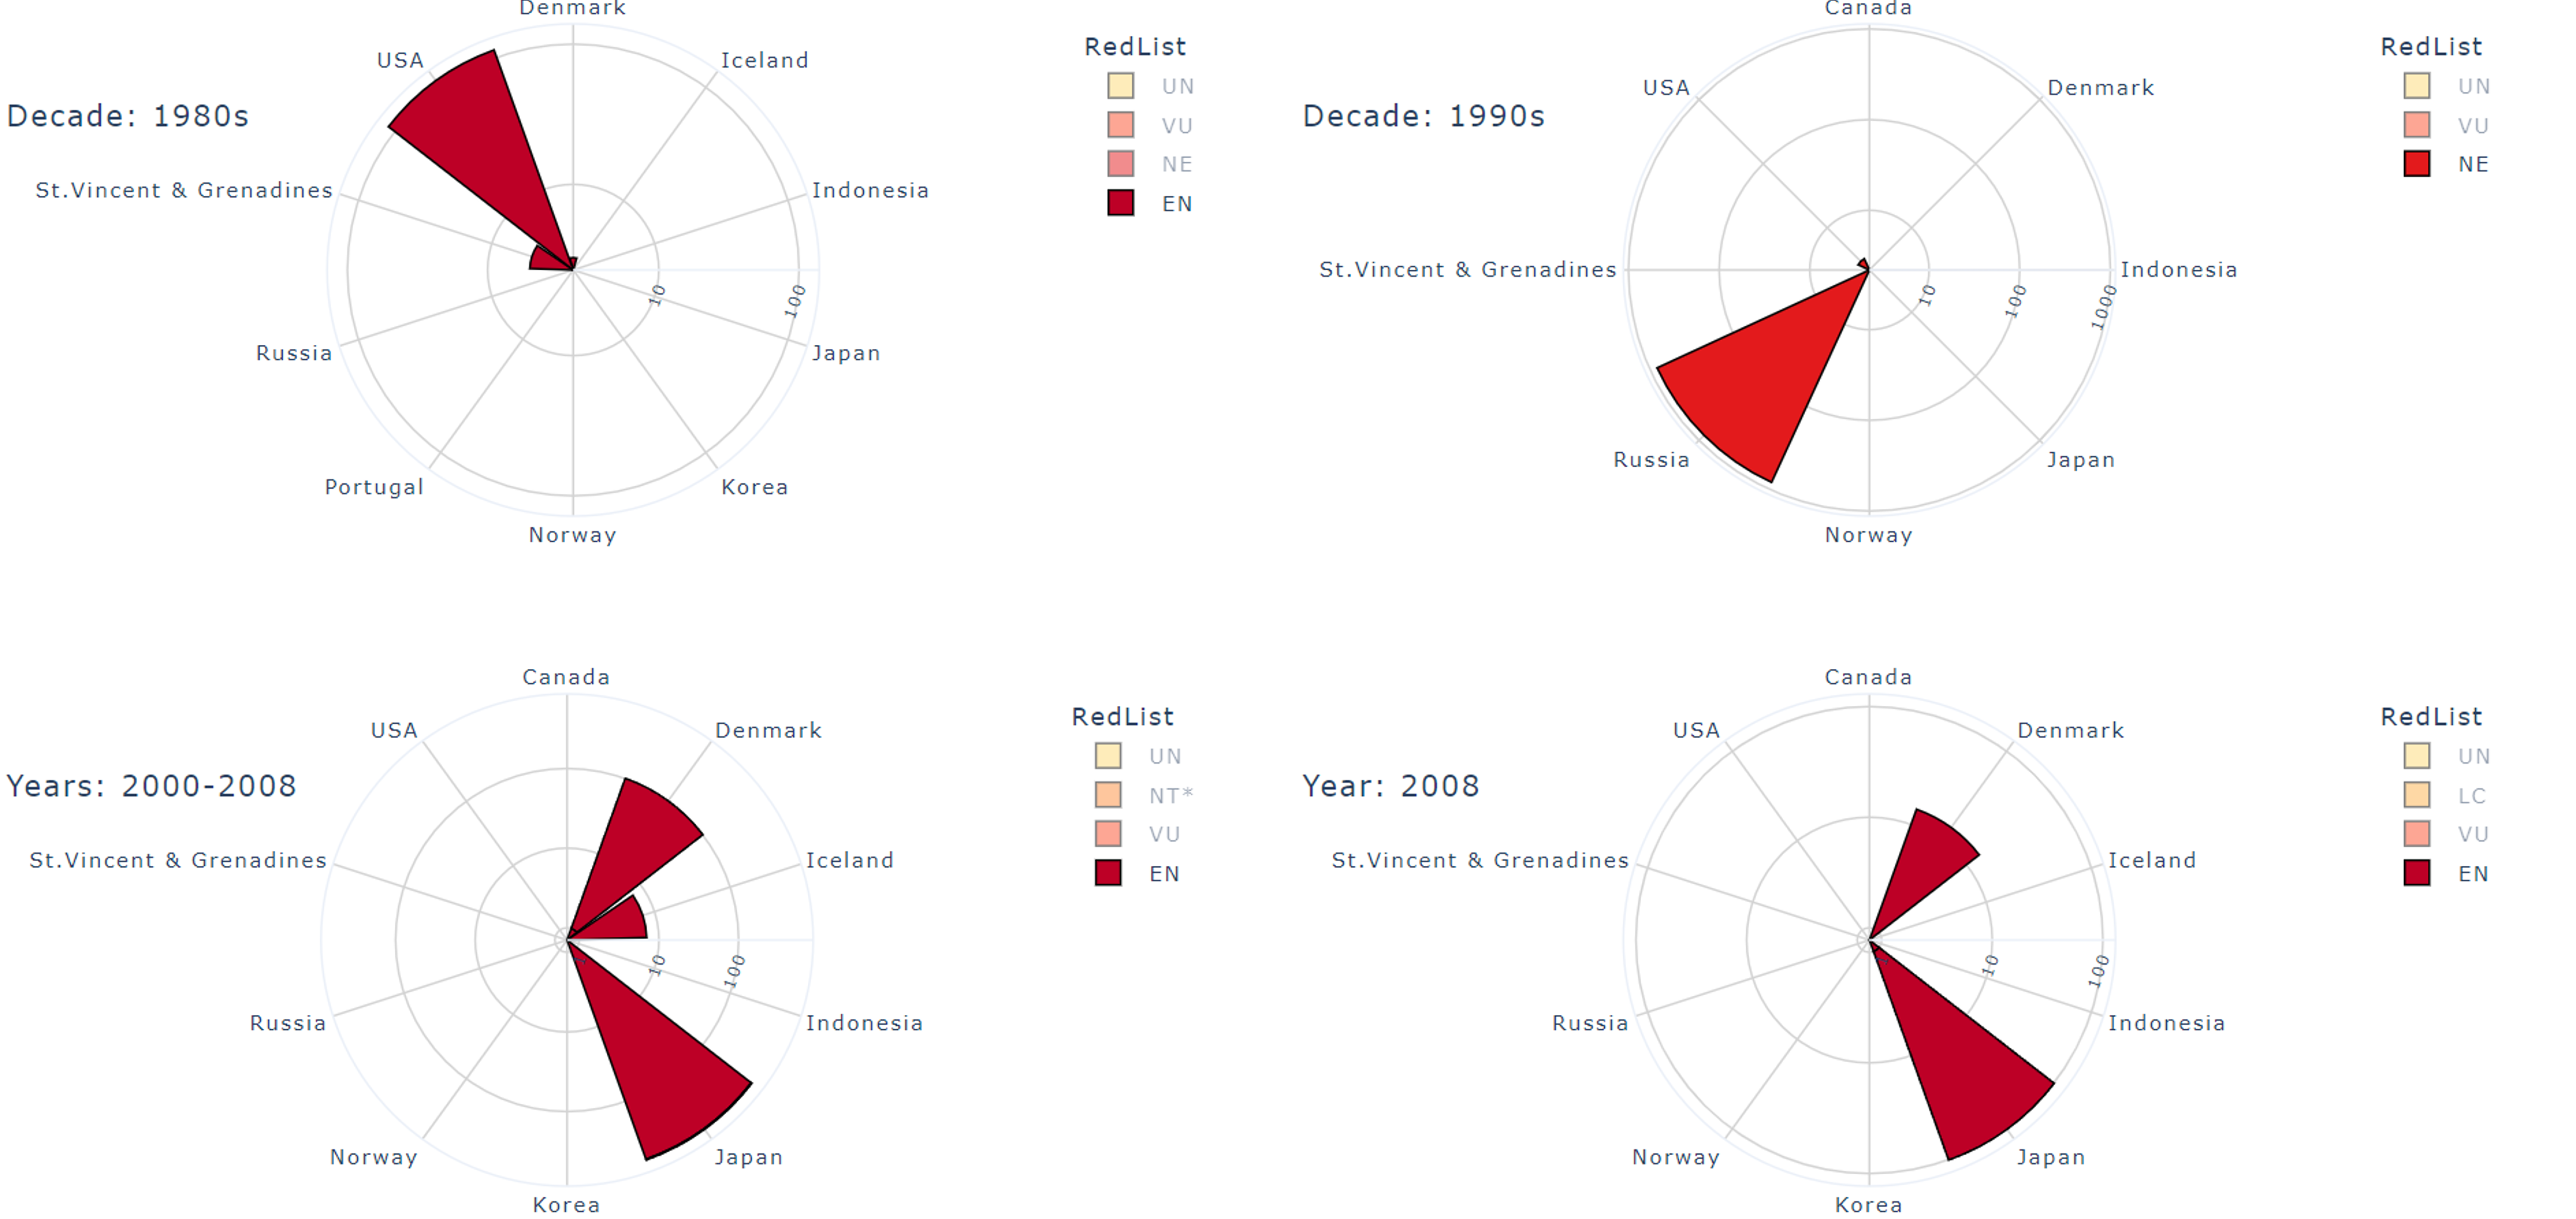
\includegraphics[width = 18cm]{PolarPlot.png}
    \caption{Final Species and Area breakdown visualisation in year 2003}
    \label{fig:my_label}
\end{figure}

\subsubsection{Evaluation}
The visualisation illustrates how the IUCN Red List criteria affects commercial whaling for particular nations. Notably, the Bowhead whale in the 1980s was listed as Endangered (EN) with 114 whaled by the United States. This number rose to 504 by the 1990s where Bowhead whale was listed as Vulnerable. This could be coincidental although a similar trend is apparent with the Sperm whale and Indonesia. This could suggest a cause-and-effect, relationship where increased numbers in whale population simply leads to an increased amount of whaling. Contrary the Minke whale is the most commonly whaled species across all decades, where it is stated that "there are likely to be several hundred
thousand individuals of this species living in the
Southern Hemisphere" (Reference). This implies why there are large catch totals for this subgroup. Although, this also suggests why it's much more difficult to derive a predictive model on the species' overall abundance, leading them to be listed as 'Data
Deficient in 2008' (reference).


\section{Univariate/Bivariate Visualisations}

\subsection{Whale Species Quantile Distribution}
As the prior visualisations explored correlations and relationships between multiple feature sets. However, a more in-depth analysis technique can be utilised to derive if two features obtain similar distributions. In particular, analysing the catch quantile distribution between species can reveal if any two species had similar catch distributions. This may aid in revealing information about the species populations within areas of catches or prompt further investigation into why the catch distribution of two species are similar. 


To visualise this quantile-quantile graphs were utilised. Initially, a quantile-quantile plot matrix was considered, allowing more efficient observation between two individual plots. However, an 8 by 8 matrix, proved to be too difficult to interpret. Therefore an interactive drop-down feature has been incorporated which allows the user to select two quantile distributions to observe. 


\begin{minted}[frame=single,framesep=4pt,fontsize=\small]{python}
qq_data = original_df.groupby(['Year'])['Fin', 'Sperm',
'Humpback', 'Sei', 'Bryde\'s', 'Minke', 'Gray', 
'Bowhead'].sum().reset_index()
q1 = qq_data[species1]
q2 = qq_data[species2]
\end{minted}

\begin{figure}[H]
    \centering
    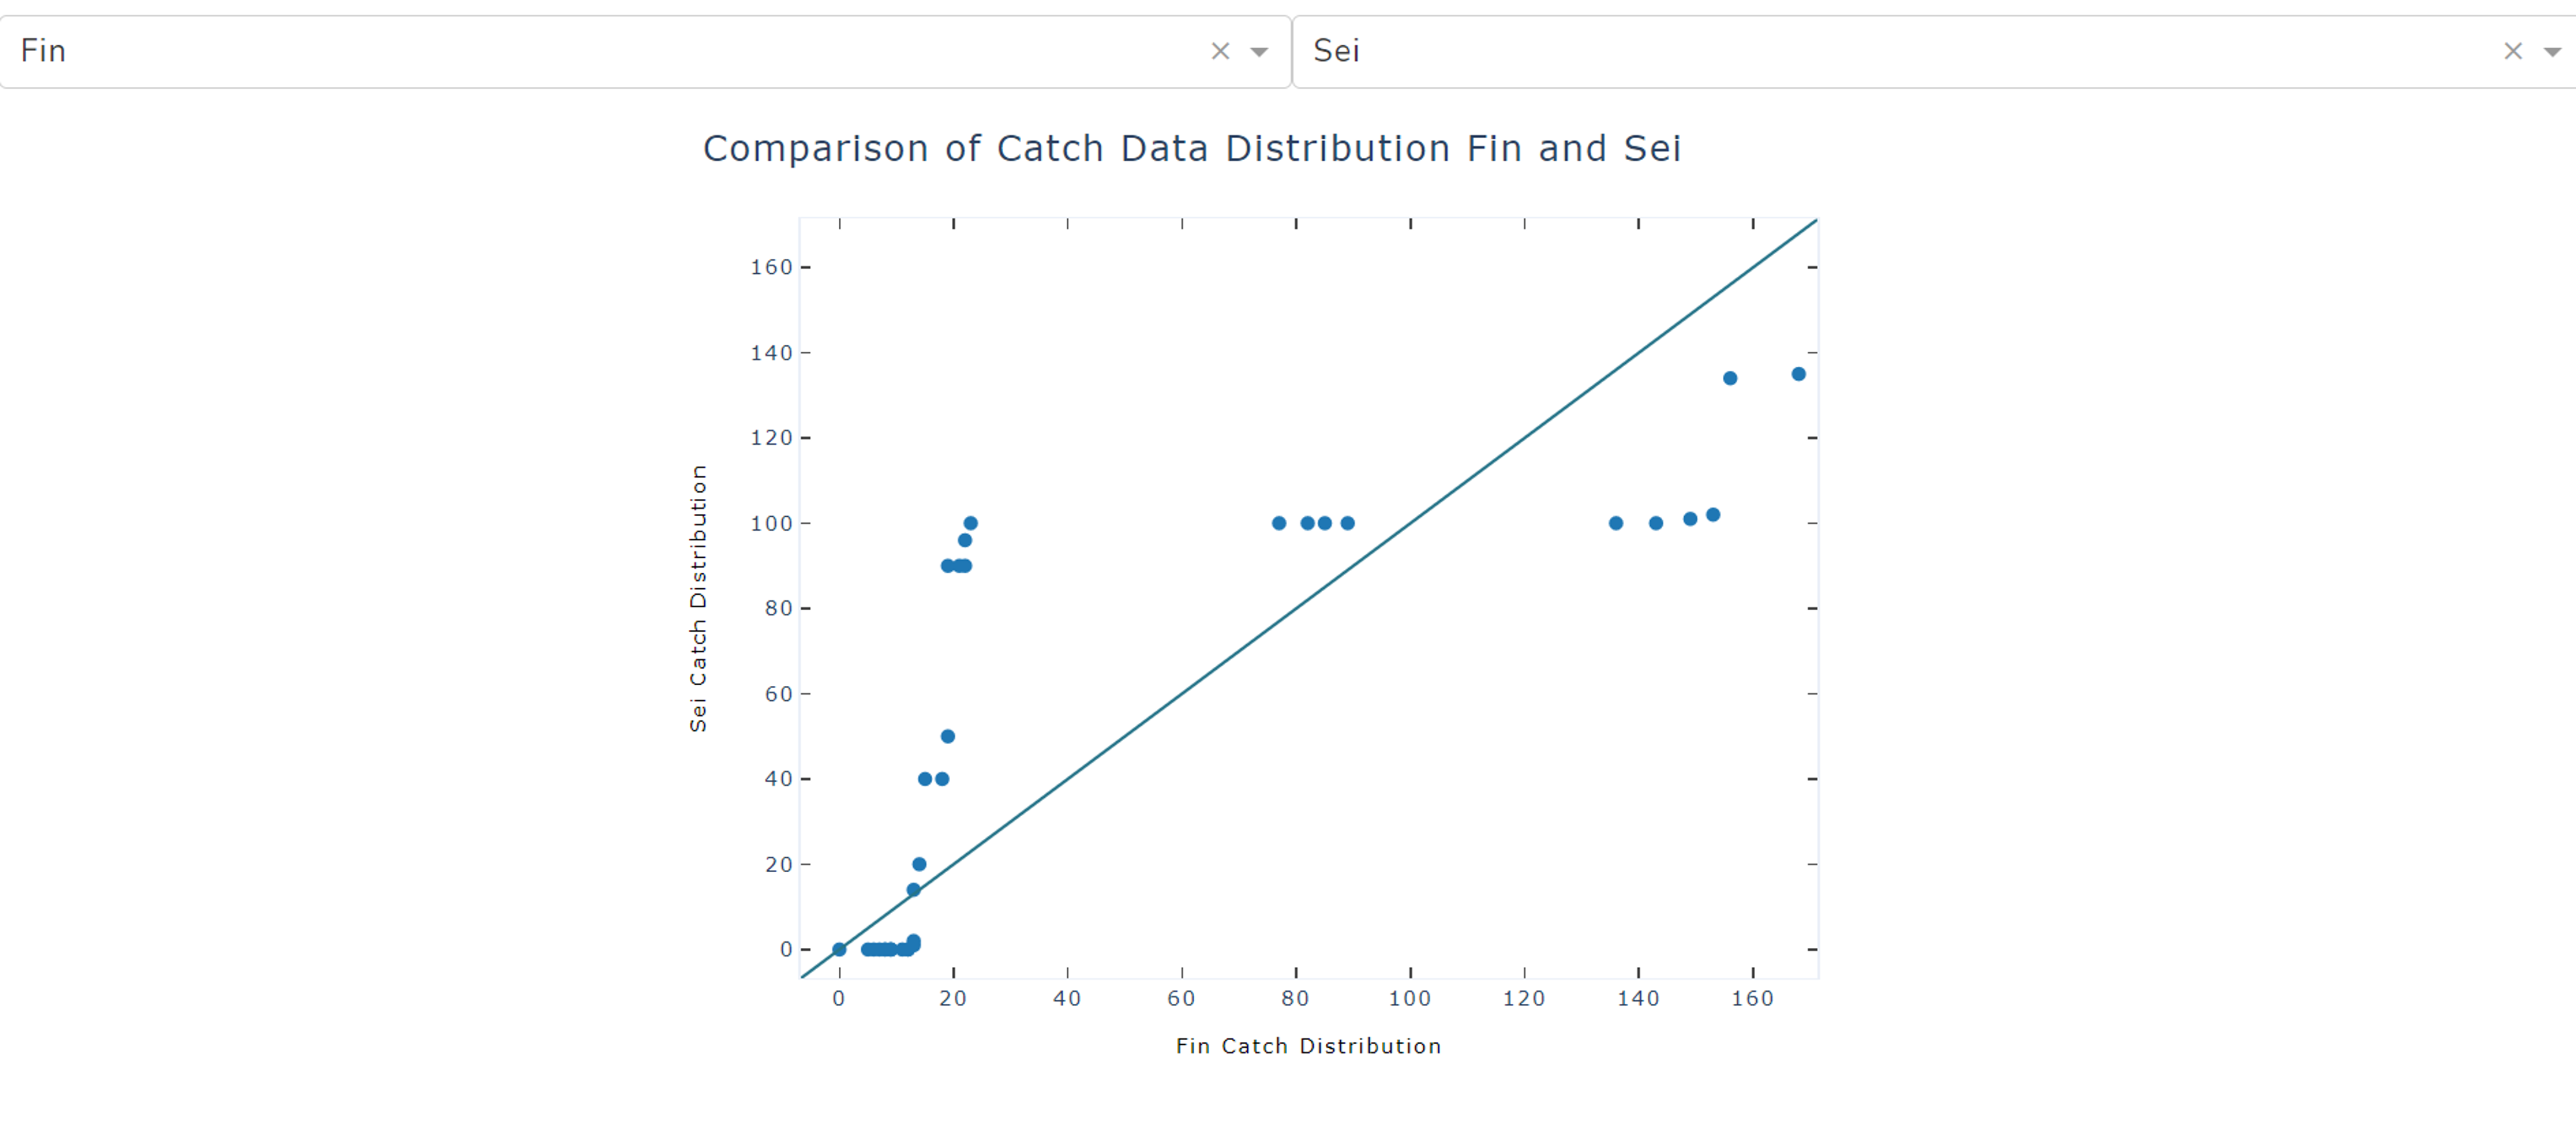
\includegraphics[width = 15cm]{Fin+Sei.png}
    \caption{Quantile-Quantile plot of Fin and Sei catch distribution}
    \label{fig:my_label}
\end{figure}

\begin{figure}[H]
    \centering
    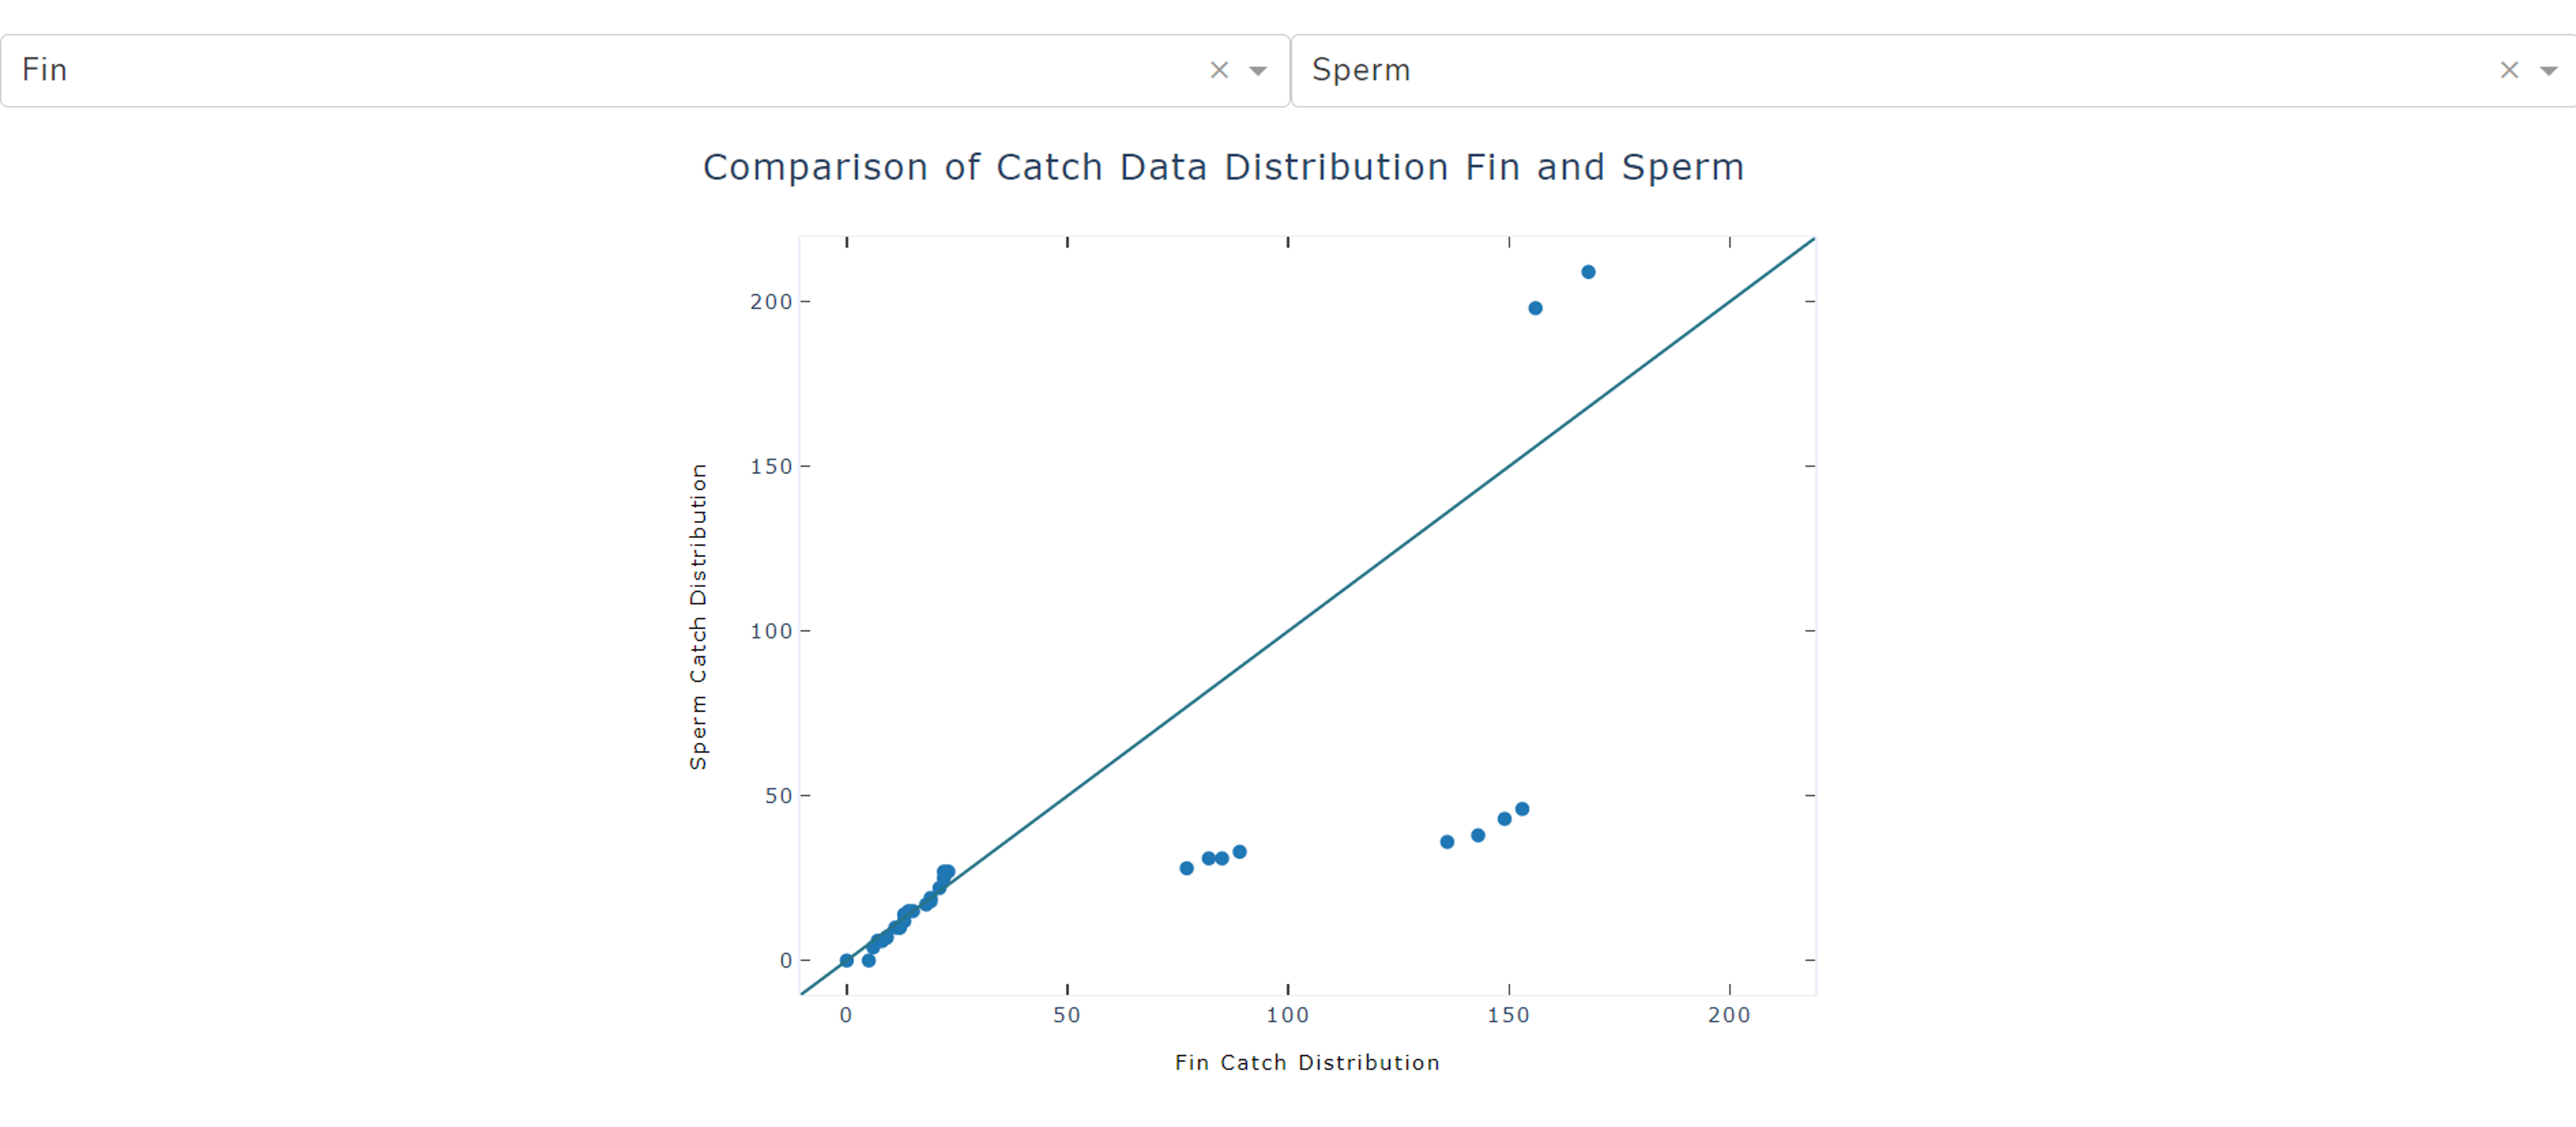
\includegraphics[width = 15cm]{Fin+Sperm.png}
    \caption{Quantile-Quantile plot of Fin and Sperm catch distribution}
    \label{fig:my_label}
\end{figure}

\subsubsection{Evaluation}
The visualisation demonstrates that some species' catch distributions are comparable and could be due to the IWC's catch sanctions restricting the number of catches or could indicate the abundance of these two species being particularly low or high. 
This is evidenced in the Fin and Sperm catch distribution, where the lower catch numbers are comparable ranging from 20 to 27. Moreover, this is further corroborated when observing the 'Area and 'Species Aggregate bar graph in Figure X. The figure highlights that in areas Japan and W. Greenland, the catches are 388 for Sperm whales and 382 for Fin whales respectively. This may indicate that across all years the catches were consistently within a range of 20 to 27 within these areas, resulting in very similar distributions. 

\begin{figure}[H]
    \centering
    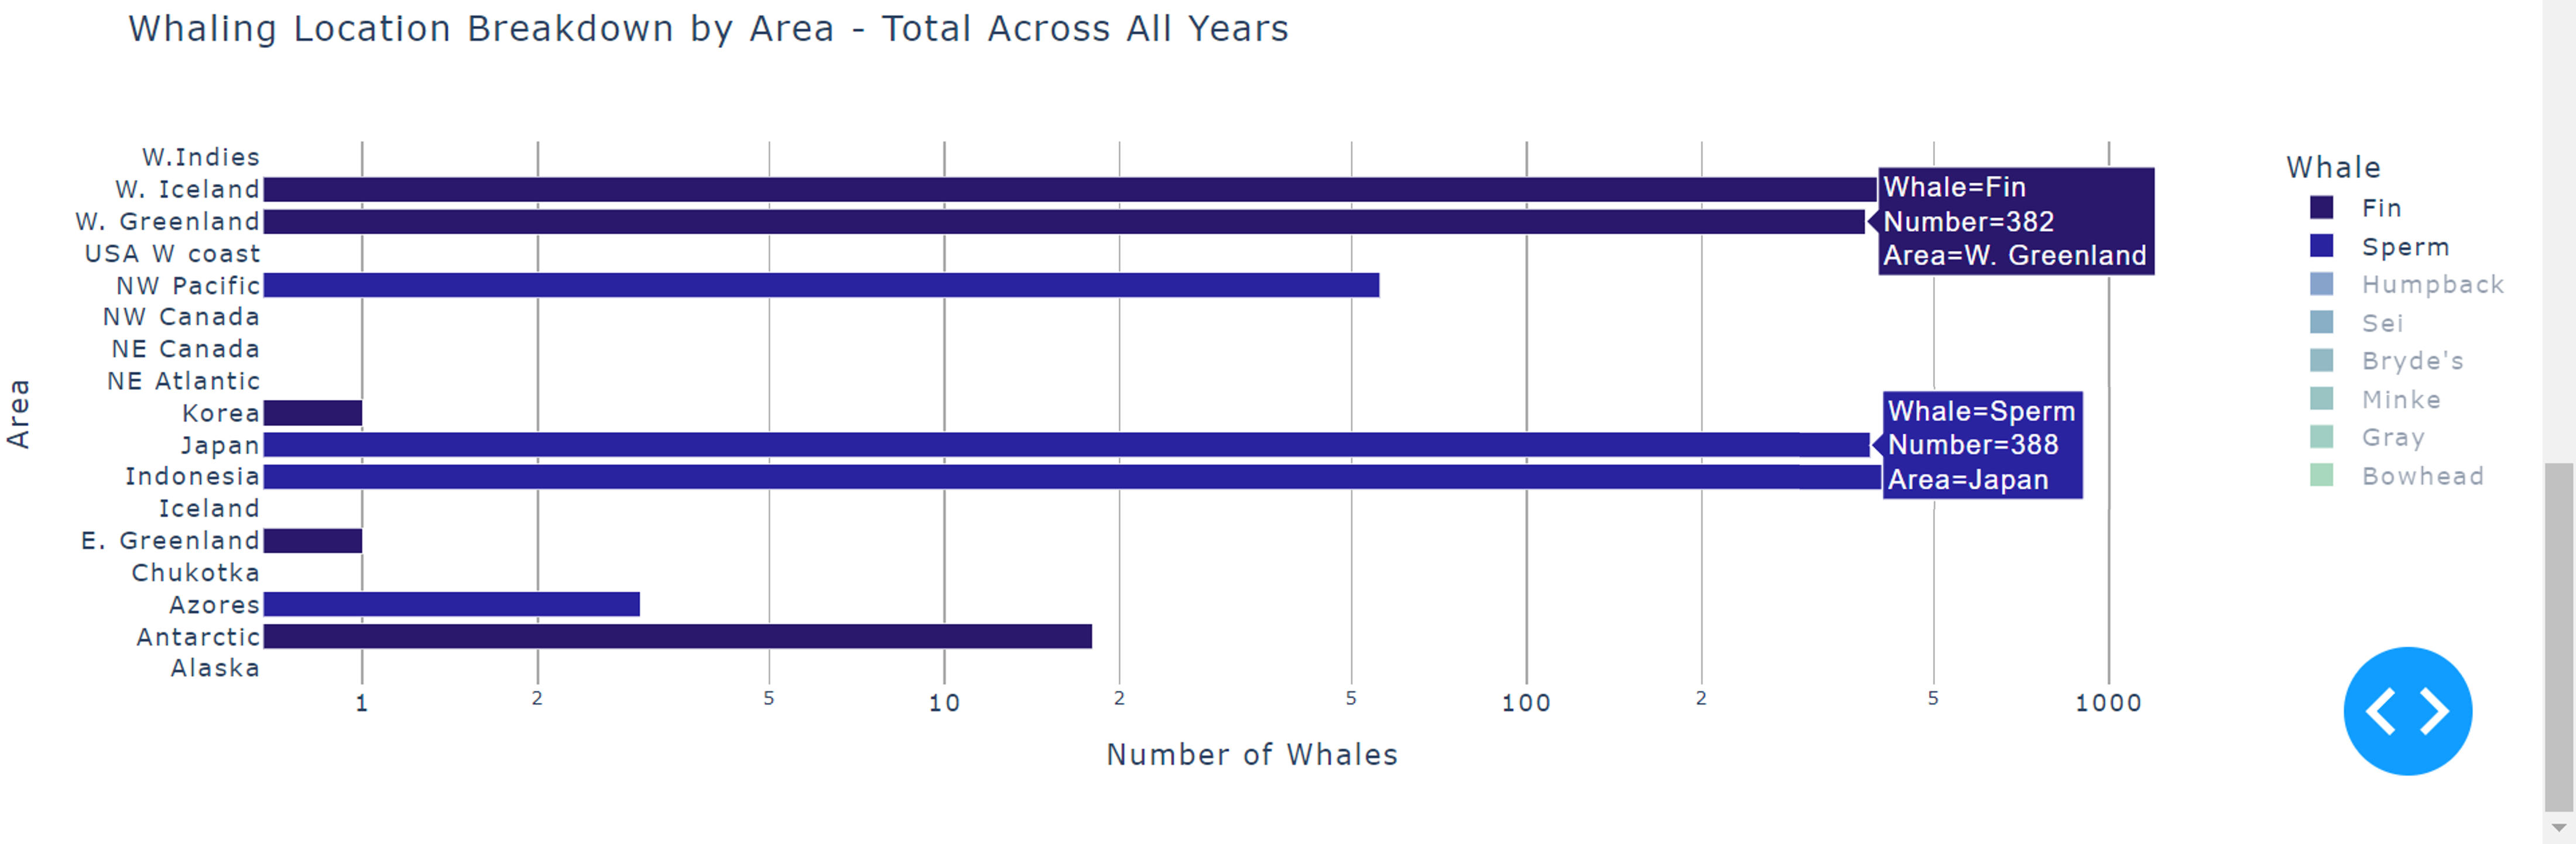
\includegraphics[width = 15cm]{Fin+SeiAreaGraph.png}
    \caption{Fin and Sei Aggregate Catch data by area}
    \label{fig:my_label}
\end{figure}


\subsection{Species Overall Distribution}
The final visualisation provides an overall quantile distribution for each species, this was best achieved utilising a box plot. The initial visualisation utilised a standard scale, which is difficult to observe, therefore a logarithmic scale was utilised for the final visualisation. However, as the logarithm of zero is undefined, the bottom half of the quantile plot isn't visible. To counteract this, a small constant of 0.0001 is added to all zero values, such that this is visible on the log scale. 

\begin{figure}[H]
    \centering
    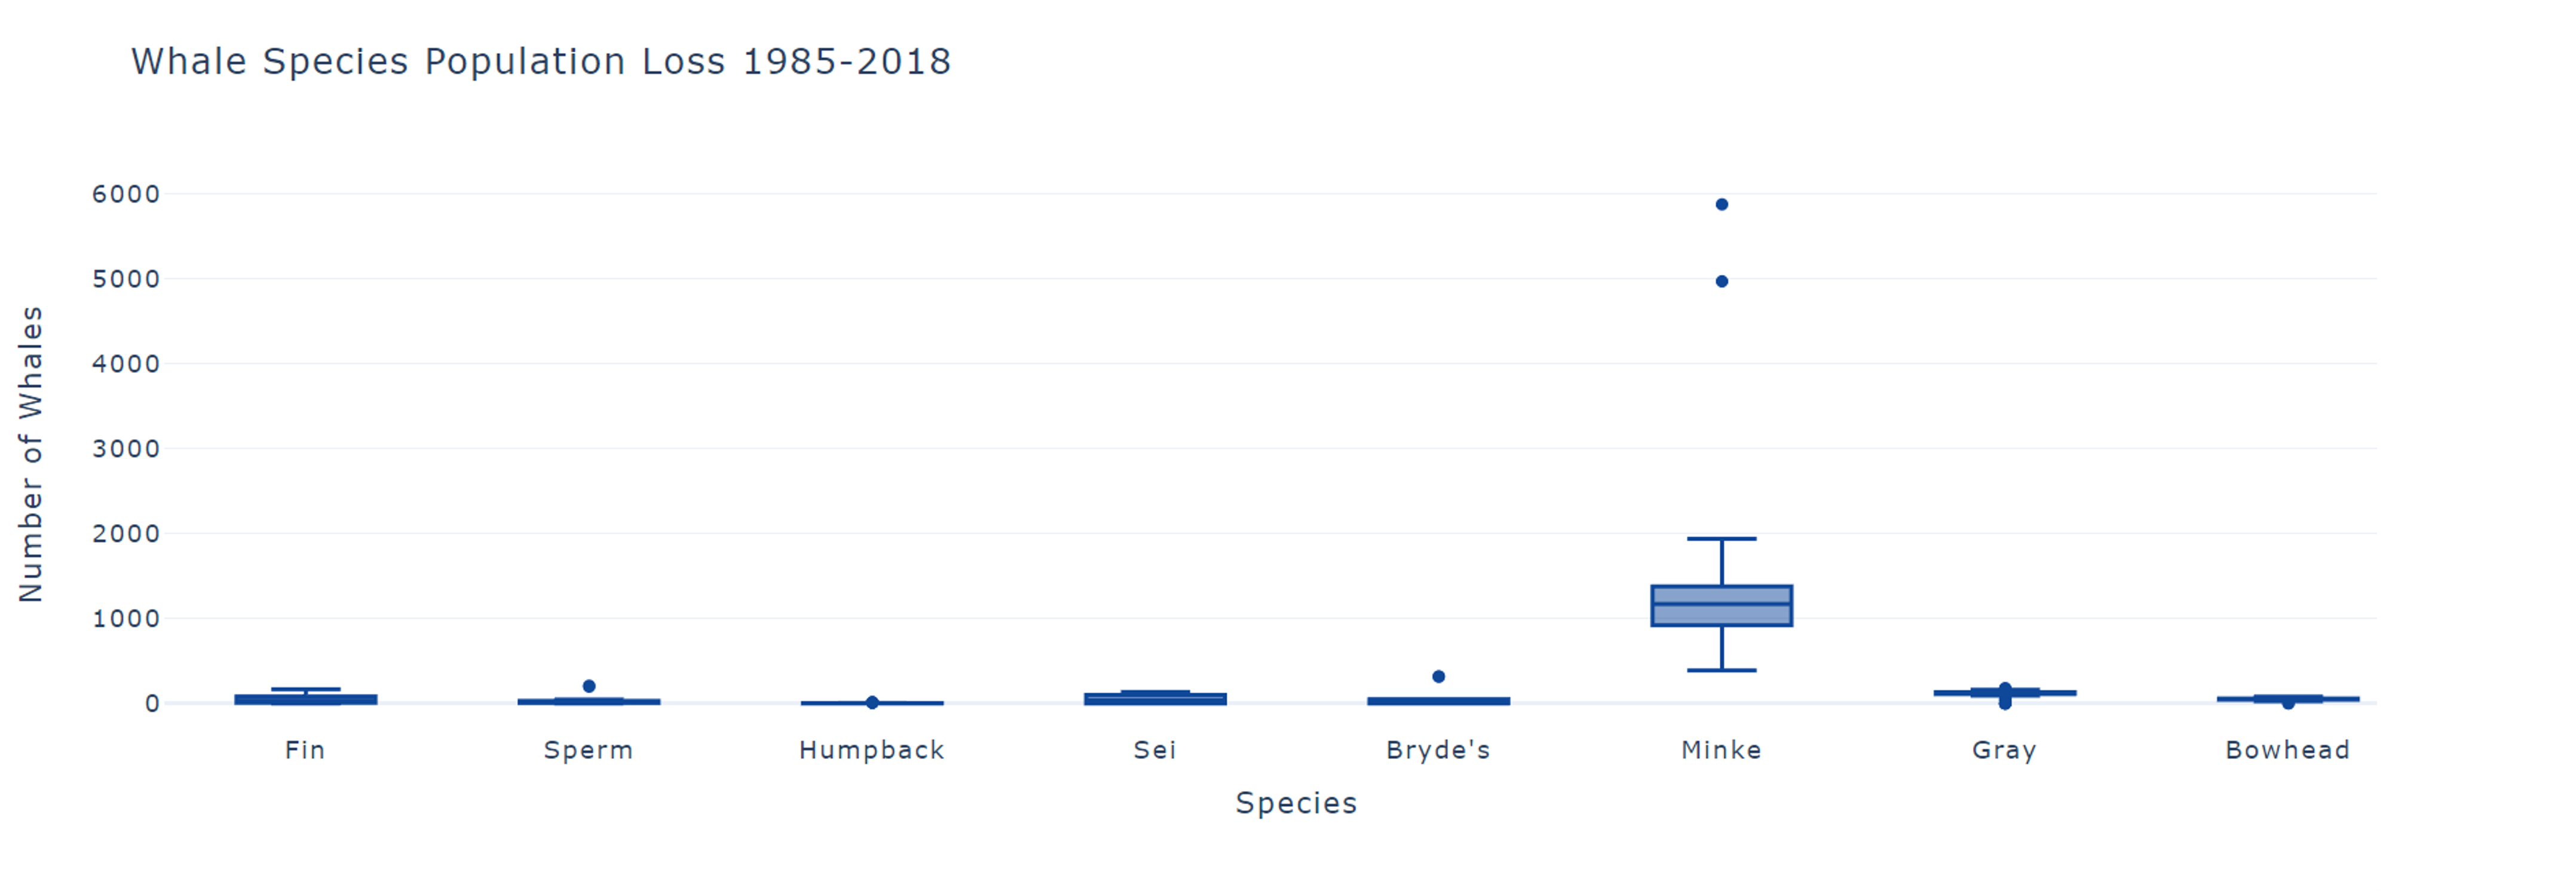
\includegraphics[width = 15cm]{boxFnoLog.png}
    \caption{Species Catch Distribution with a non-logarithmic scale}
    \label{fig:my_label}
\end{figure}

\begin{figure}[H]
    \centering
    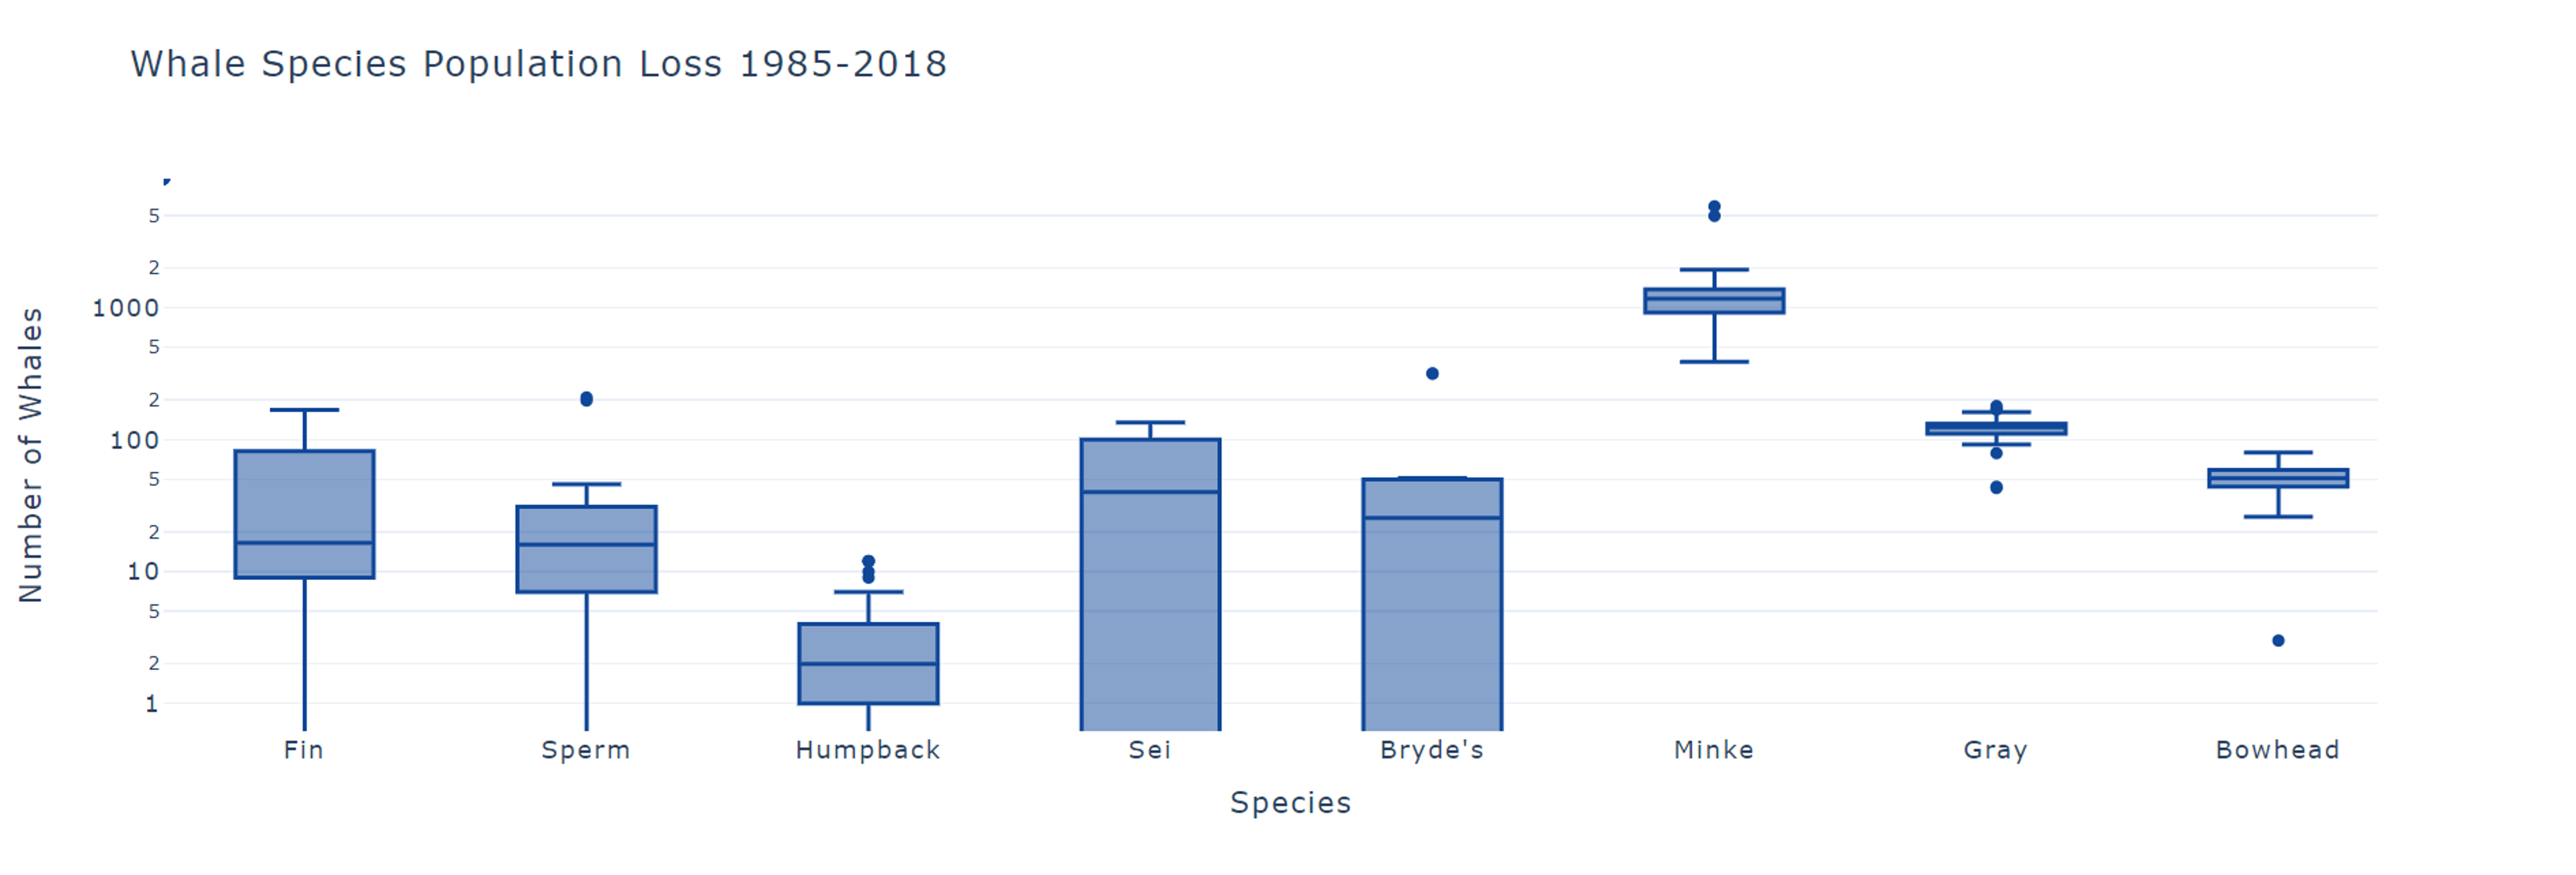
\includegraphics[width = 15cm]{boxFlog.png}
    \caption{Species Catch Distribution with a logarithmic scale}
    \label{fig:my_label}
\end{figure}

\subsubsection{Evaluation}
This further assists the above quantile distribution, as species that appear to have similar box plots may be granularly explored above with the quantile-quantile plot. Contrary species such as the Minke whale that has a fairly skewed distribution may not be comparable with any other species. Additionally, this visualisation is transferable for print viewing. 


\section{Discussion}

\subsection{Unsuccessful Visualisations}

The below Principal Component Analysis was conducted by reducing the feature set dimension of the various whale species. This was in order to gauge the distribution or range of whales for each Nation across time. As PCA would assist in demonstrating the variance across the feature sets. 

However, the visualisation can be denoted as unsuccessful as there aren't any obvious clusters or distributions that the data portrays.

\begin{figure}[H]
    \centering
    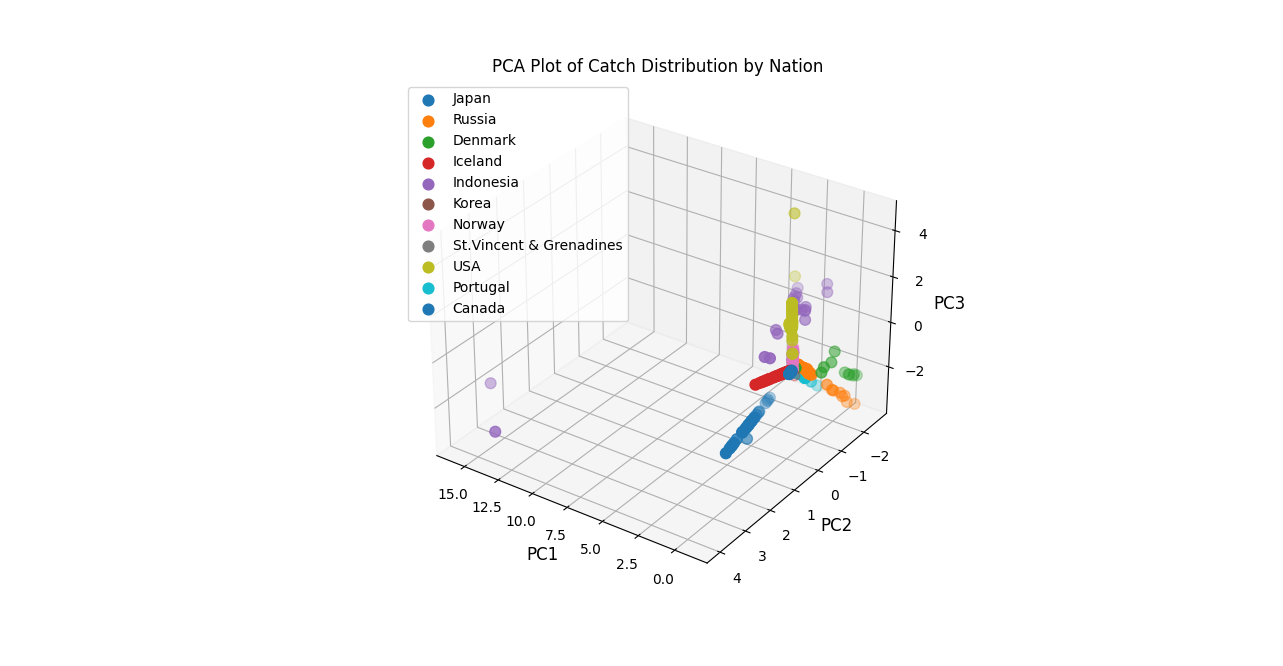
\includegraphics[width = 15cm]{Figure_2.png}
    \caption{Principal Component Analysis of Whaling Species Distribution by Nation}
    \label{fig:my_label}
\end{figure}

\subsection{Colour Palette Selection}
The disadvantage of the set of visualisations is the large reliance on colours, where additional dimensionality was commonly providing using colours. Therefore, it was essential to accommodate for individuals with vision impairments that could affect the visualisation's effectiveness. 
The two main colour palettes utilised for the visualisations were the plotly express's sequential YlORd palette and the Haline palette.  A sequential palette was utilised as the colours vary in hue, and brightness. This continuous gradient scale ensures that colours can be distinguished between one another, where the variation in hues and allows for transferrability when printing in grayscale. This is evidenced in Figure X. 


\noindent
\begin{figure}[H]
     \centering
     \begin{subfigure}[b]{0.45\textwidth}
         \centering
         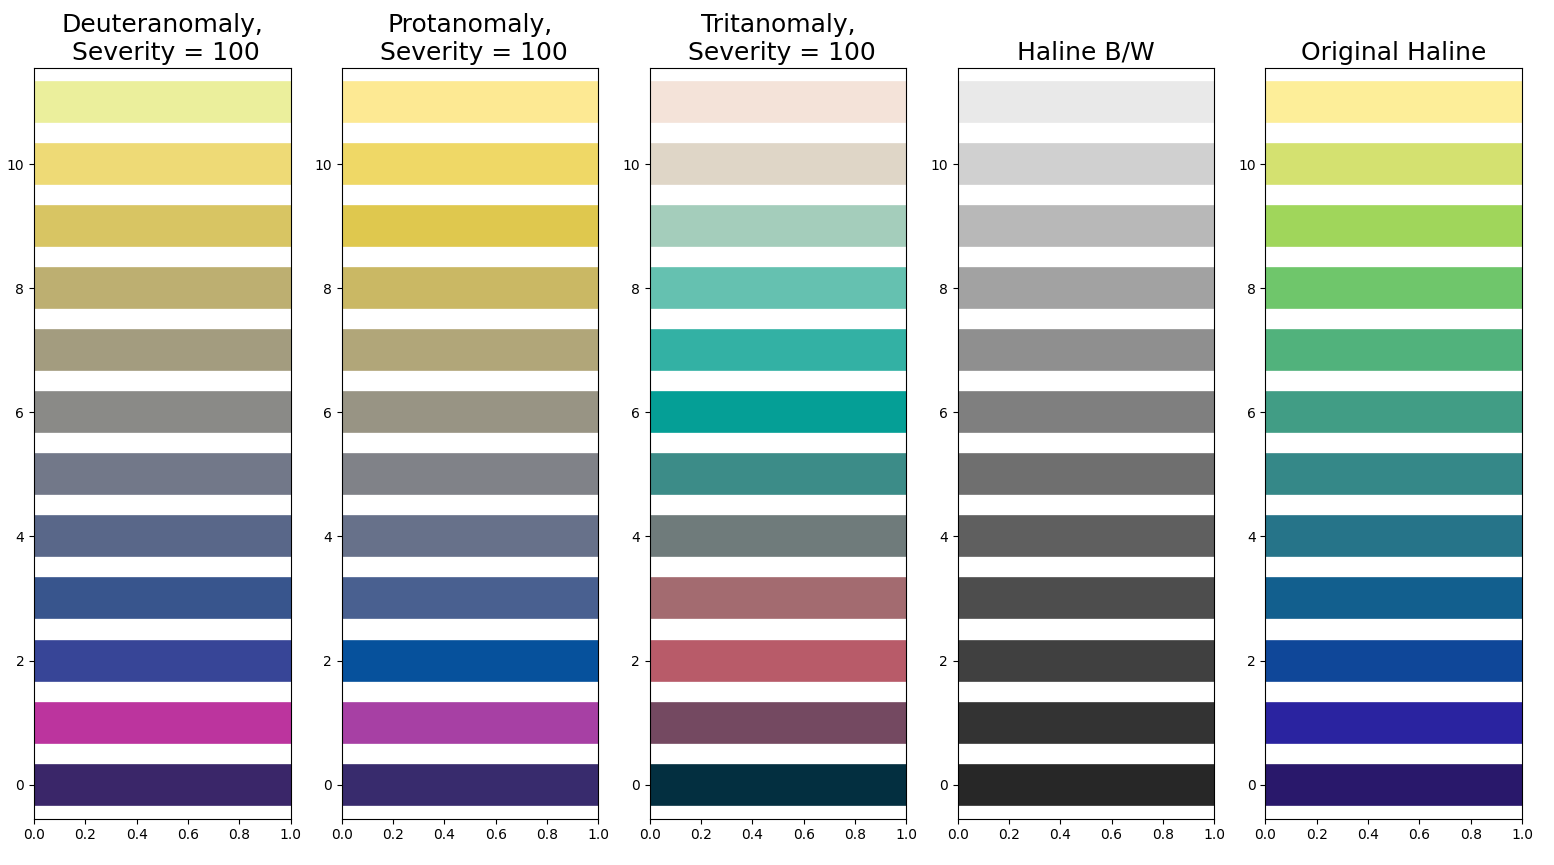
\includegraphics[width=\textwidth]{colour_blindness_haline.png}
         \caption{$y=x$}
         \label{fig:y equals x}
     \end{subfigure}
     \hfill
     \begin{subfigure}[b]{0.45\textwidth}
         \centering
         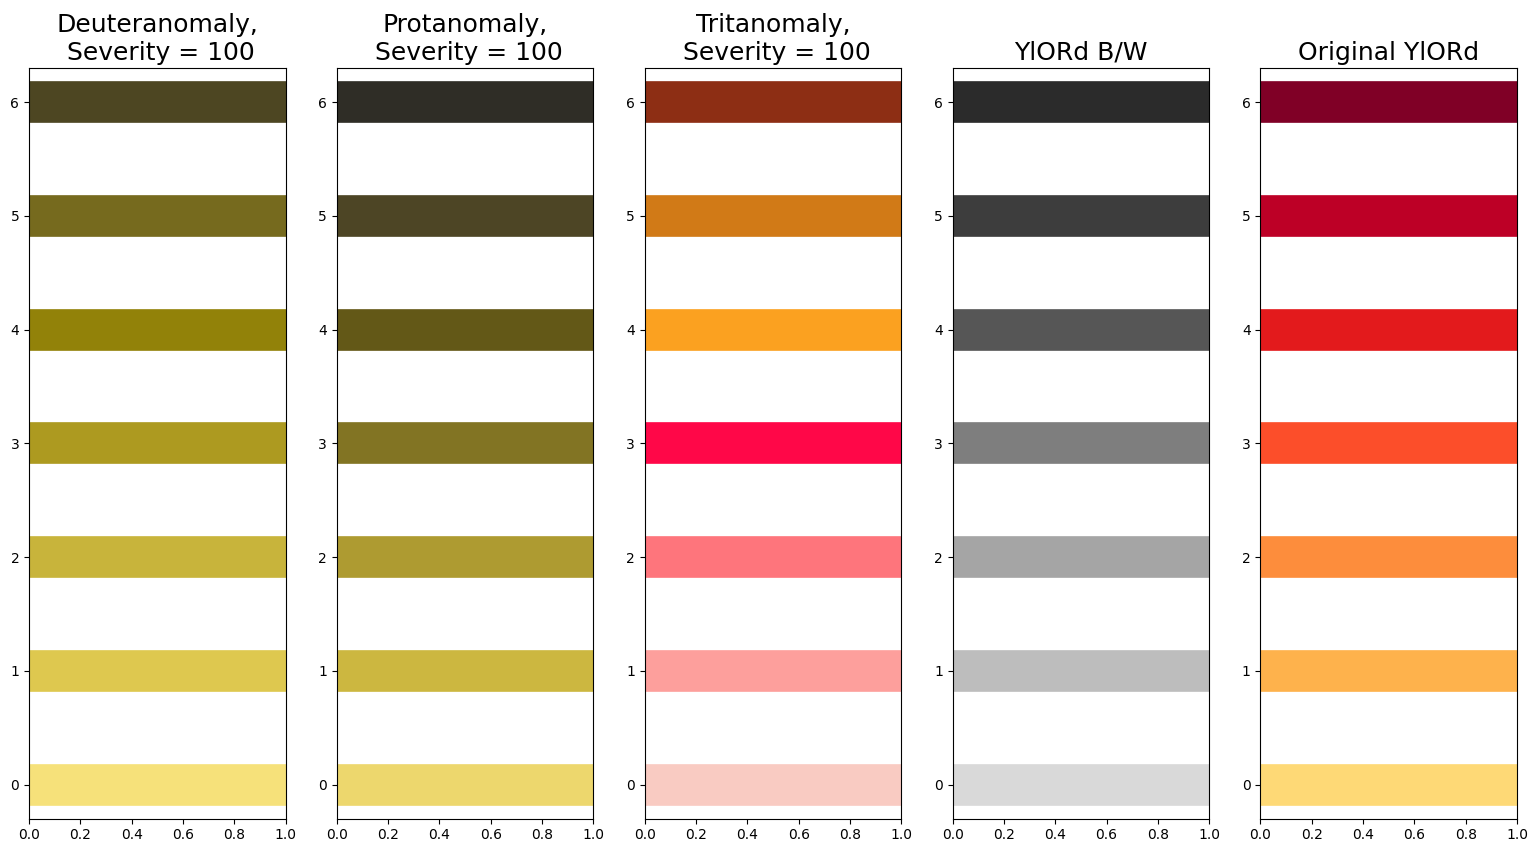
\includegraphics[width=\textwidth]{red_palette.png}
         \caption{$y=3\sin x$}
         \label{fig:three sin x}
     \end{subfigure}
\end{figure}

Notably, the YlORd palette proves to be distinguishable for across the three types of colour blindness along with being relatively transferrable for gray scale. Although it does propose a level of difficulty for the Deuteranomaly class of individuals with shades 5 and 4 being quite similar. 

Contrary, haline colours whilst avoid red and green contrasts by utilising a subtle hue variation, the colours 5, 6 and 7, are definitely much more difficult to distinguish. Although the palette does cater to the colour blind class of Deutanomaly and Protanomaly. To cater for the distinguishing of colours a \textbf{'Change Theme'} button has been included which provides a dark background, allowing for colour contrasts to become much more visible, as opposed to the contrast against a white background. This is evidenced in Figure X. 

\begin{figure}[H]
    \centering
    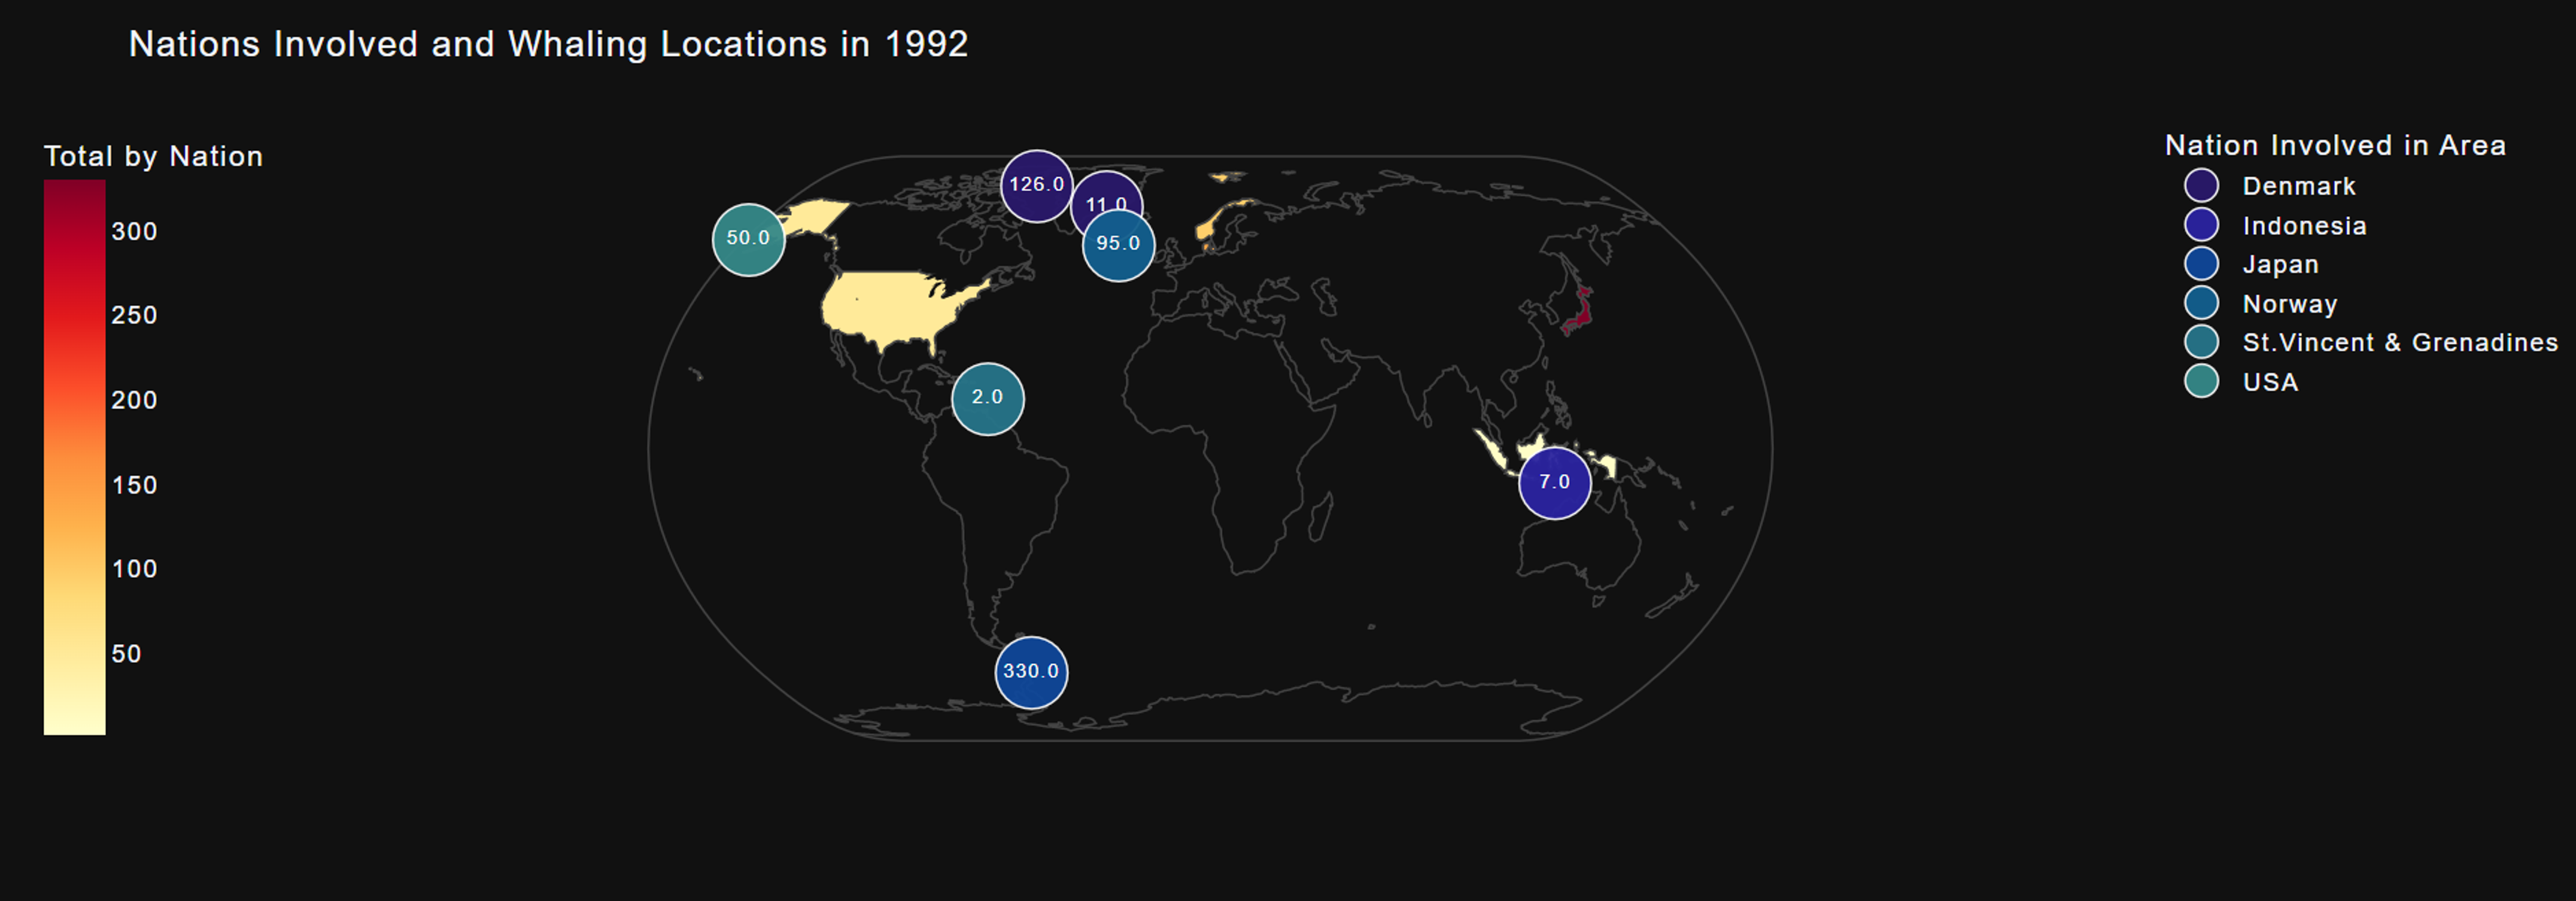
\includegraphics[width = 12cm]{ChoroDark.png}
    \caption{Principal Component Analysis of Whaling Species Distribution by Nation}
    \label{fig:my_label}
\end{figure}

% \pagebreak
% \begin{landscape}
\subsection{Dashboard Layout}
To further assist in ease of viewing, the provided scope visualisations have been grouped into 'Tabs', creating an overall interactive dashboard interface.

\begin{figure}[H]
    \centering
    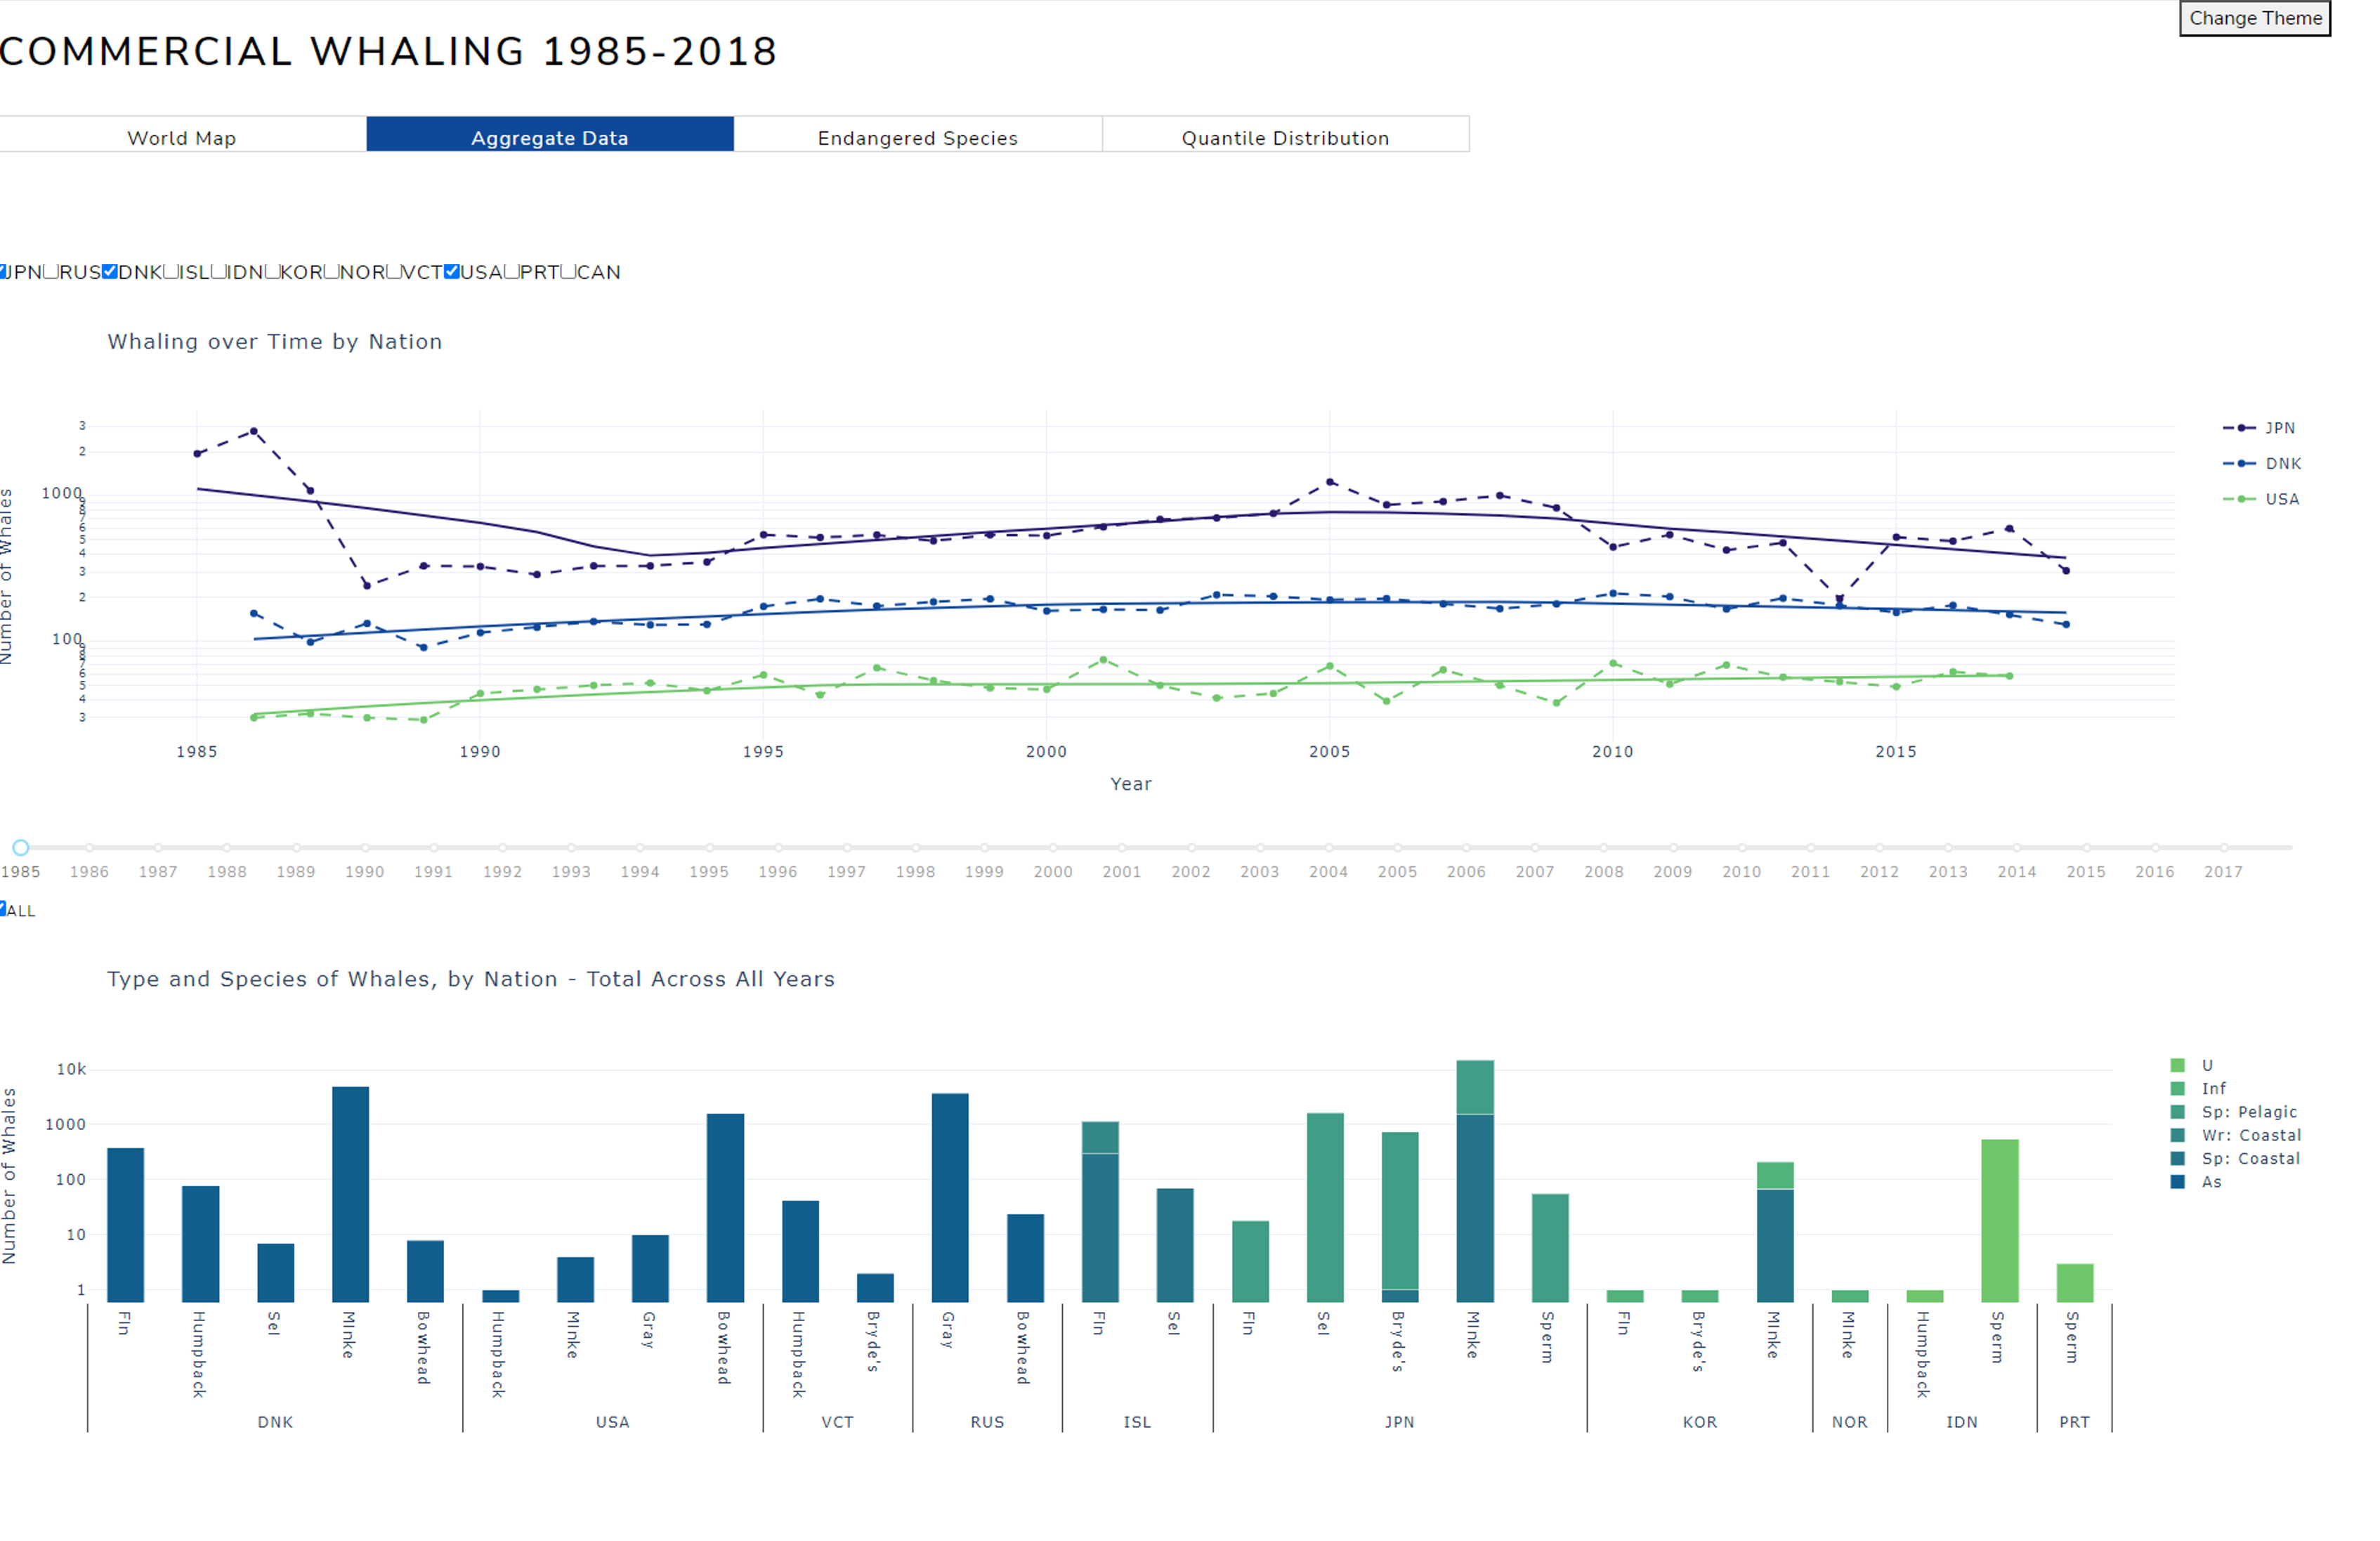
\includegraphics[width = 14cm]{DashboardLayout.png}
    \caption{Caption}
    \label{fig:my_label}
\end{figure}
% \end{landscape}

\subsection{Reccomendations}
Final recommendations for the visualisations include exploring how else multi-dimensionality can be represented without the use of colour. This would aid in limiting the number of categorical features, thereby alleviating the need for colour to distinguish between 10 or more features. This could have been achieved by combining the data set with another data set that was more continuous in nature, creating opportunities for other data analysis techniques to be employed. However, the resources available on commercial whaling are fairly limited and quite confidential. 
% \newpage


\section{Conclusion}
In conclusion, the set of visualisations is intended to educate and inform individuals on the history of commercial whaling, along with it's overall trajectory and what potential preventative measures need to be in place. Evidently whaling has seen a considerable reduction over time, where it each Nation appears to stay within a particular range of total catches. This may assist with further predictive modelling on species abundances. Furthermore, the goegraphical visualisation aided in establishing how Type classifications are curated, and how Nation's typically whale regionally with the exception of Japan and Russia who conduct whaling in various locations across the globe. 
Lastly, distribution greatly assisted in observing the overall skew and similarities between species distributions. 
Overall, the project can be denoted as successful in providing creative achieving its desired intentions, where 

\newpage

\nocite{BNCC}

\bibliography{bibliografia}  %Preencha o arquivo bibliografia.bib com as referência adequadamente formatadas (pesquise sobre arquivos de extensão .bib) e descomente esta linha para que aparecem já em formato ABNT

\section{Appendices}

\subsection{Appendix A}
\begin{table}[H]
\centering
\caption{Geographical Areas}
\begin{tabular}{|c|c|c|}
\hline
Area & Latitude & Longitude \\
\hline
Antarctic & -62.9569253 & -60.6328425 \\
\hline
Alaska & 58.1769992 & -167.136665 \\
\hline
Chukotka & 69.4467673 & -171.3853847 \\
\hline
E. Greenland & 68.4275896 & -32.55215 \\
\hline
Indonesia & -9.6004834 & 121.7535375 \\
\hline
Japan & 28.056319 & 149.4087118 \\
\hline
NE Atlantic & 56.5499995 & -24 \\
\hline
Korea & 37.253807 & 131.2362315 \\
\hline
W. Iceland & 64.9098481 & -21.9188185 \\
\hline
W.Indies & 13.6571919 & -60.8986297 \\
\hline
NW Canada & 52.2595533 & -129.7790971 \\
\hline
NE Canada & 53.8878796 & -53.5909151 \\
\hline
Azores & 35.5721322 & -25.3726121 \\
\hline
NW Pacific & 31.3900266 & -156.550517 \\
\hline
Iceland & 65.6750207 & -9.0916241 \\
\hline
USA W coast & 29.1130403 & -128.4039841 \\
\hline
W. Greenland & 75.3906409 & -66.8595852 \\
\hline
\end{tabular}
\label{tab:geographical_areas}
\end{table}

\subsection{Appendix B}
\begin{table}[h]
\centering
\caption{Conservation Status of Selected Whale Species}
\begin{tabular}{|c|c|c|c|c|}
\hline
Species & 1980s & 1990s & 2000 - 2008 & 2008 \\
\hline
Gray & NE & NE & NT* & LC \\
\hline
Sei & NE & VU & EN & EN \\
\hline
Fin & VU & VU & EN & EN \\
\hline
Humpback & EN & VU & VU & LC \\
\hline
Sperm & NE & VU & VU & VU \\
\hline
Bowhead & EN & VU & NT* & LC \\
\hline
Minke & UN & UN & UN & UN \\
\hline
Bryde’s & UN & UN & UN & UN \\
\hline
\end{tabular}
\label{tab:whale_species}
\end{table}

\newpage
\subsection{Appendix C}

\begin{minted}[frame=single,framesep=4pt,fontsize=\small]{python}
def alpha3code(column):
    CODE=[]
    for country in column:
        try:
            # print(country)
            if(country == "USSR"):
                
                country == "USSR, Union of Soviet Socialist Republics"
                code=pycountry.countries.get(alpha_3='RUS').alpha_3
            elif(country == "St.Vincent & Grenadines"):
                code = pycountry.countries.get(name="Saint Vincent and the 
                Grenadines").alpha_3
            elif(country == "Korea"):
                code = pycountry.countries.get(name='Korea, Republic of').alpha_3
            elif(country == "Russia"):
                 code = pycountry.countries.get(name='Russian 
                 Federation').alpha_3
            elif(country == "USA"):
               code = pycountry.countries.get(alpha_3='USA').alpha_3
            else:
                code=pycountry.countries.get(name=country).alpha_3

            CODE.append(code)
        except:
            CODE.append('None')
    return CODE
\end{minted}

\subsection{Appendix D}
\begin{minted}[frame=single,framesep=4pt,fontsize=\small]{python}
#Storing Longitude and Latitude coordinates based on Area
latitudes = []
longitudes = []

for d in df_1['Area']:
    for a,b,c in zip(locations['Area'],locations['Latitude'],
    locations['Longitude']):
        if(a==d):
            latitudes.append(b)
            longitudes.append(c)
df_1['latitudes'] = latitudes
df_1['longitudes'] = longitudes
\end{minted}

\newpage
\subsection{Appendix E}
\begin{minted}[frame=single,framesep=4pt,fontsize=\small]{python}
original_df_2 = pd.read_csv("Project\\WhalingData.csv").dropna()
original_df_2['Nation'].replace({"USSR": "Russia"}, inplace=True)
original_df_2['Type'] = original_df_2['Type'].str.title()

# Iterate through each decade (1980s, 1990s, 2000s, and 2008)
for decade in [1980, 1990, 2000, 2008]:
    # Filter the dataframe to only include rows from the current decade
    if decade == 2000:
        decade_df = original_df_2[(original_df_2['Year'] >= decade) & 
        (original_df_2['Year'] < decade+9)] # Years 2000 to 2008
    elif decade == 2008:
         decade_df = original_df_2[original_df_2['Year'] ==decade] #Year 2008
         alone
    else:
        decade_df = original_df_2[(original_df_2['Year'] >= decade) & 
        (original_df_2['Year'] < decade+10)] #1980s and 1990s

    # Create a dictionary to hold the country-specific data for this decade
    country_dict = {}

    # Iterate through each country in the current decade
    for country in decade_df['Nation'].unique():
        # Filter the dataframe to only include rows for the current country
        country_df = decade_df[decade_df['Nation'] == country]
        # Calculate the total number of each whale species for the current country
        whale_counts = {}
        for species in ['Fin', 'Sperm', 'Humpback', 'Sei', "Bryde's", 'Minke',
        'Gray', 'Bowhead']:
            whale_counts[species] = country_df[species].sum()
        # Add the whale counts to the dictionary for the current country
        country_dict[country] = whale_counts
    # Add the country-specific data to the dictionary for the current decade

    decades_dict[f"{decade}s"] = country_dict
\end{minted}


\end{document}
